% **************************************************
% Clean Thesis
% -- A LaTeX Style for Thesis Documents --
%
% Copyright (C) 2011-2015 Ricardo Langner
% **************************************************
%
% Readme:
% ----------------------------------------
% Please check out the README.md file in the root of this package.
%
%
% License Information:
% ----------------------------------------
% "Clean Thesis" is free software: you can redistribute it and/or modify
% it under the terms of the GNU General Public License as published by
% the Free Software Foundation, either version 3 of the License, or
% (at your option) any later version.
%
% "Clean Thesis" is distributed in the hope that it will be useful,
% but WITHOUT ANY WARRANTY; without even the implied warranty of
% MERCHANTABILITY or FITNESS FOR A PARTICULAR PURPOSE.  See the
% GNU General Public License for more details.
%
% You should have received a copy of the GNU General Public License
% along with this program.  If not, see <http://www.gnu.org/licenses/>.
% **************************************************

%\newcommand{\LeDraft}{true}
\newcommand{\LeDraft}{false}

% **************************************************
% Document Class Definition
% **************************************************
\documentclass[%
	paper=A4,					% paper size --> A4 is default in Germany
	twoside=true,				% onesite or twoside printing
	openright,					% doublepage cleaning ends up right side
	parskip=full,				% spacing value / method for paragraphs
	chapterprefix=true,			% prefix for chapter marks
	10pt,						% font size
	headings=normal,			% size of headings
	bibliography=totoc,			% include bib in toc
	listof=totoc,				% include listof entries in toc
	titlepage=on,				% own page for each title page
	captions=tableabove,		% display table captions above the float env
	draft=\LeDraft,				% value for draft version
]{scrreprt}%

% **************************************************
% Debug LaTeX Information
% **************************************************
%\listfiles

% **************************************************
% Load and Configure Packages
% **************************************************
\usepackage[T1]{fontenc}
\usepackage[utf8]{inputenc}
\usepackage{lmodern}


% **************************************************
% Information and Commands for Reuse
% **************************************************
\newcommand{\thesisTitle}{Personalized Perception and Interaction with Medical Information in Mixed Reality Environments}
%Personalized Interaction with Medical Information in Mixed Reality Environments
%Personalisierte Interaktion mit Medizinischen Informationen in Mixed Reality Umgebungen
\newcommand{\thesisName}{Meng Ma}
\newcommand{\thesisSubject}{Dissertation}
\newcommand{\thesisDate}{\today}
\newcommand{\thesisVersion}{1.0}

\newcommand{\thesisVorsitzender}{..............................}
\newcommand{\thesisVorsitzenderAffiliation}{ }

\newcommand{\thesisFirstReviewer}{Prof. Nassir Navab, Ph.D.}
\newcommand{\thesisFirstReviewerAffiliation}{
	Technische Universität München\\[-1mm]
	Computer Aided Medical Procedures
}

\newcommand{\thesisSecondReviewer}{Prof. Hongen LIAO, Ph.D}
\newcommand{\thesisSecondReviewerAffiliation}{
	 Tsinghua University, School of Medicine\\[-1mm]
	 Department of Biomedical Engineering,
}

\newcommand{\thesisFirstSupervisor}{Prof. Nassir Navab}
\newcommand{\thesisSecondSupervisor}{Dr. Pascal Fallavollita}

\newcommand{\thesisUniversity}{\protect{Technische Universität München}}
\newcommand{\thesisUniversityDepartment}{Fakultät für Informatik}
\newcommand{\thesisUniversityInstitute}{Lehrstuhl für Informatikanwendungen in der Medizin \& Augmented Reality}
\newcommand{\thesisUniversityGroup}{}
\newcommand{\thesisUniversityCity}{Garching bei München}
\newcommand{\thesisUniversityStreetAddress}{Boltzmannstraße 3}
\newcommand{\thesisUniversityPostalCode}{85748}


% **************************************************
% Load and Configure Packages
% **************************************************
\usepackage[english]{babel} 	% babel system, adjust the language of the content
\usepackage[					% clean thesis style
	figuresep=colon,%
	sansserif=false,%
	hangfigurecaption=true,%
	hangsection=true,%
	hangsubsection=true,%
	colorize=full,%
	colortheme=bluemagenta,
	draft=\LeDraft				% value for draft version
]{cleanthesis}

\hypersetup{					% setup the hyperref-package options
	pdftitle={\thesisTitle},	% 	- title (PDF meta)
	pdfsubject={\thesisSubject},% 	- subject (PDF meta)
	pdfauthor={\thesisName},	% 	- author (PDF meta)
	plainpages=false,			% 	-
	colorlinks=false,			% 	- colorize links?
	pdfborder={0 0 0},			% 	-
	breaklinks=true,			% 	- allow line break inside links
	bookmarksnumbered=true,		%
	bookmarksopen=true			%
}

\usepackage[					    % use biblatex for bibliography
	backend=bibtex,		      		% 	- use biber backend (bibtex replacement) or bibtex
	bibencoding=utf8,				% 	- use auto file encode
	style=numeric,				% 	- use alphabetic (or numeric) bib style
	natbib=true,					% 	- allow natbib commands
	hyperref=true,					% 	- activate hyperref support
	backref=true,					% 	- activate backrefs
	isbn=false,						% 	- don't show isbn tags
	url=false,						% 	- don't show url tags
	doi=false,						% 	- don't show doi tags
	urldate=long,					% 	- display type for dates
	maxnames=3,%
	minnames=1,%
	maxbibnames=5,%
	minbibnames=3,%
	maxcitenames=2,%
	mincitenames=1,%
	defernumbers=true%
]{biblatex}
\bibliography{E:/TUM_Narvis/documents/BibTex/library}
\newcommand{\citeName}[1]{ \citeauthor{#1}\cite{#1}}
\makeatletter

\newrobustcmd*{\parentexttrack}[1]{%
	\begingroup
	\blx@blxinit
	\blx@setsfcodes
	\blx@bibopenparen#1\blx@bibcloseparen
	\endgroup}

\AtEveryCite{%
	\let\parentext=\parentexttrack%
	\let\bibopenparen=\bibopenbracket%
	\let\bibcloseparen=\bibclosebracket}

\makeatother

\usepackage{amsmath}
\usepackage{amssymb}
\usepackage{multirow}

\usepackage{tabu}
\usepackage{array}
\usepackage{booktabs}
\usepackage{multirow}
\usepackage{gensymb}
\renewcommand{\arraystretch}{1.5}		% set vertical line padding to factor 1.5
\setlength{\tabcolsep}{8pt}				% set the column separation (6pt is default)
\setlength{\heavyrulewidth}{0.10em}		% set the thickness of the top and bottom rules

\newcolumntype{L}{>{\raggedright\arraybackslash}X}
\newcolumntype{R}{>{\raggedleft\arraybackslash}X}
\newcolumntype{C}{>{\centering\arraybackslash}X}
\usepackage{geometry}
\usepackage{pdflscape}

\usepackage{tikz}
%% !TEX root = ../thesis-example.tex
%

% load needed libraries
\usetikzlibrary{calc,trees,positioning,arrows,chains,shadows,fit,shapes,shadings,decorations.pathmorphing}

\pgfdeclarelayer{background}
\pgfdeclarelayer{foreground}
\pgfdeclarelayer{1}
\pgfdeclarelayer{2}
\pgfdeclarelayer{3}
\pgfdeclarelayer{4}
\pgfdeclarelayer{5}
\pgfsetlayers{background,main,foreground,1,2,3,4,5}

% define a fancy color map (inspired by Visifire)
\definecolor{MyColor1}{RGB}{67, 134, 216}
\definecolor{MyColor2}{RGB}{255, 154, 46}
\definecolor{MyColor3}{RGB}{219, 68, 63}
\definecolor{MyColor4}{RGB}{168, 212, 79}
\definecolor{MyColor5}{RGB}{133, 96, 179}
\definecolor{MyColor6}{RGB}{60, 191, 227}
\definecolor{MyColor7}{RGB}{234, 212, 32}

\definecolor{tumblue}{rgb}{0, 0.5, 0.75}
\definecolor{ocker}{RGB}{119, 112, 95}

\tikzset{%
	source/.style={%
		top color=white, bottom color=green!20, draw=green!75!black!75%
	},%
	sink/.style={%
		top color=white, bottom color=red!20, draw=red!75!black!65%
	},%
	schritt-base/.style={%
		rectangle, rounded corners=1.5mm, drop shadow, %
		align=center, %
		thick, draw=ctcolormain!75, %
		top color=white, bottom color=ctcolormain!30,%
		font=\sffamily\scriptsize%
	},%
	entity-base/.style={%
		chamfered rectangle, chamfered rectangle sep=0.75mm, chamfered rectangle corners={north east}, drop shadow, %
		align=center, %
		thick, draw=black!20, %
		top color=white, bottom color=black!10,%
		font=\sffamily\scriptsize%
	}, %
	pfeil/.style={%
		|-, ->, very thick%
		,draw=MyColor2, >=stealth'%
		,{rounded corners}%
	},%
}

\newcommand{\PORT}[4]{%
	\coordinate (#1) at #2;%
	\filldraw [draw=white, fill=#3] (#1) circle (1mm) #4;%
}


\usepackage{rotating}
\usepackage{ifthen}
\usepackage{subfig}
\usepackage{wrapfig}
\usepackage{enumitem}
\usepackage{threeparttable}
\usepackage{pifont}% http://ctan.org/pkg/pifont
\usepackage{soul}
\usepackage{xspace}
\newcommand{\cmark}{\ding{51}}%
\newcommand{\xmark}{\ding{55}}%
\newcolumntype{P}[1]{>{\centering\arraybackslash}p{#1}}
\captionsetup[subfigure]{format=plain,labelsep=space,singlelinecheck=true}

% **************************************************
% More custom commands
% **************************************************
\newcommand{\add}[1]{{\color{black}{#1}}} 
\newcommand{\addd}[1]{{\color{black}{#1}}}  %blue
%\newcommand{\add}[1]{#1} 
%\newcommand{\addd}[1]{#1} 
\newcommand{\TODO}[1]{{\bfseries\textsl{\textcolor{red}{[#1]}}}}
\newcommand{\CN}{\TODO{citation needed}}
\newcommand{\RA}{\TODO{Review again}}
\newcommand{\II}{{\bfseries\textsl{\textcolor{RubineRed}{[insert image]}}}}
\newcommand{\III}[1]{{\bfseries\textsl{\textcolor{RubineRed}{[insert image: #1]}}}}
\newcommand{\SYN}[1]{{\bfseries\textsl{\textcolor{OliveGreen}{[#1?]}}}}
\newcommand*{\eg}{e.g.\@\xspace}
\newcommand*{\ie}{i.e.\@\xspace}

\makeatletter
\newcommand*{\etc}{%
	\@ifnextchar{.}%
	{etc}%
	{etc.\@\xspace}%
}
\makeatother

% **************************************************
% Document CONTENT
% **************************************************
\begin{document}

% --------------------------
% rename document parts
% --------------------------
%\renewcaptionname{ngerman}{\figurename}{Abb.}
%\renewcaptionname{ngerman}{\tablename}{Tab.}
\renewcaptionname{english}{\figurename}{Figure }
\renewcaptionname{english}{\tablename}{Table }

% --------------------------
% Front matter
% --------------------------
%recover the following comment after you finish the main contents
\pagenumbering{roman}			% roman page numbing (invisible for empty page style)
\pagestyle{empty}				% no header or footers
% !TEX root = ../thesis-example.tex
%
% ------------------------------------  --> cover title page
\begin{titlepage}
	\pdfbookmark[0]{Cover}{Cover}
	\flushright
	\hfill
	\vfill
	{\LARGE\thesisTitle \par}
	\rule[5pt]{\textwidth}{.4pt} \par
	{\Large\thesisName}
	\vfill
	\textit{\large\thesisDate} \\
	Version: \thesisVersion
\end{titlepage}


% ------------------------------------  --> main title page
\begin{titlepage}
	\pdfbookmark[0]{Titlepage}{Titlepage}
	\tgherosfont
	\centering

	
\includegraphics[width=4cm]{gfx/TUM_logo.pdf} \\[2mm]
	{\Large \thesisUniversity} \\
	\textsf{\thesisUniversityDepartment} \\
	\textsf{\thesisUniversityInstitute} \\
	\textsf{\thesisUniversityGroup} \\

	\vfill
	{\LARGE \color{ctcolortitle}\textbf{\thesisTitle} \\[10mm]}
	{\Large \thesisName} \\

	\vfill
	\begin{minipage}[t]{.95\textwidth}
		Vollständiger Abdruck der von der Fakultät für Informatik der Technischen Universität München zur Erlangung des akademischen Grades eines
		\begin{center}
			Doktors der Naturwissenschaften (Dr. rer. nat.)
			\end{center}
			genehmigten Dissertation.
	\end{minipage}
	
	\vspace{1cm}

	\begin{minipage}[t]{.32\textwidth}
		\raggedleft
		\textit{Vorsitzende(r):}
	\end{minipage}
	\hspace*{15pt}
	\begin{minipage}[t]{.6\textwidth}
		{\Large \thesisVorsitzender} \\
		{\small \thesisVorsitzenderAffiliation}
	\end{minipage} \\[5mm]
	\begin{minipage}[t]{.32\textwidth}
		\raggedleft
		\textit{Prüfer der Dissertation:}
	\end{minipage}
	\hspace*{15pt}
	\begin{minipage}[t]{.6\textwidth}
		{\Large \thesisFirstReviewer} \\
		{\small \thesisFirstReviewerAffiliation}  \\[10pt]
		%
		{\Large \thesisSecondReviewer} \\
		{\small \thesisSecondReviewerAffiliation}
	\end{minipage}
	
	\vspace{1cm}
	
	\begin{minipage}[t]{.95\textwidth}
		Die Dissertation wurde am \dots\dots\dots\dots\dots\dots ~bei der Technischen Universität München eingereicht und durch die Fakultät für Informatik am \dots\dots\dots\dots\dots\dots ~angenommen.
	\end{minipage}

\end{titlepage}

% ------------------------------------  --> lower title back for single page layout
\hfill
\vfill
{
	\small
	\textbf{\thesisName} \\
	\textit{\thesisTitle} \\
	\thesisSubject, \thesisDate \\
	Reviewers: \thesisFirstReviewer\ and \thesisSecondReviewer \\
	Supervisors: \thesisFirstSupervisor\ and \thesisSecondSupervisor \\[1.5em]
	\textbf{\thesisUniversity} \\
	\thesisUniversityDepartment \\
	\thesisUniversityInstitute \\
	\thesisUniversityStreetAddress \\
	\thesisUniversityPostalCode\ and \thesisUniversityCity
}
		% INCLUDE: all titlepages
\cleardoublepage

\pagestyle{plain}				% display just page numbers
% !TEX root = Clean-Thesis.tex
%
\pdfbookmark[0]{Abstract}{Abstract}
\chapter*{Abstract}
\label{sec:abstract}
%\vspace*{-10mm}

%computer education, Mixed Reality, medical image, interaction, and perception. 

%Personal Perception and Interaction with Medical information in magic mirror framework

At first, a magic mirror framework is presented creating a MR environment with an \textit{in-situ} augmented reality view. The system can track the current user and finish the registration between the medical datasets and the user based on the personal information. It inherently allows the user to perform interactive registration and directly map the medical information onto his/her body. This opens interesting possibilities for personalized mixed reality for medical education and rehabilitation. Through the participation of 7 clinicians and 72 anatomy students, two user studies were designed to respectively assess the precision and acceptability of the magic mirror system for anatomy education in the classrooms of tomorrow. We also take the advantage of the interactive mixed reality to generate a personalized learning procedure. In addition, ``Organ Explosion'' and ``self-control virtual view'' systems are designed and implemented for anatomy leaning. Serious games are also developed in the framework for health-care education and rehabilitation exercise.
Their benefit has been shown for both educational and clinical applications.

Then, a method is proposed to calculate a virtual eye center as the origin for the \textit{eye-rooted} pointing ray technique without tracking the eye gaze in an egocentric setting. The user specific pointing geometry can then be recovered for interaction with ambient media and objects without visual feedback. The pointing ray starts from the virtual eye center and goes through the fingertip to the desired target information. During the initial calibration, the user is asked to perform pointing gestures towards several targets displayed within the field of view. A user specific virtual eye center is then estimated based on the detected fingertip in the coordinate system of the wearable device. Then the \textit{eye-rooted} pointing ray is recovered when a user is performing a pointing gesture. 
The proposed method is mathematically analyzed and determined that the calibration is feasible with a measured accuracy of the recovered pointing ray below $0.9\degree$.
The method is also evaluated in a user study consisting of 10 participants performing pointing interaction with objects shown on the display while wearing a RGB-D sensor. The study shows that the calibration is independent of the environment and the pointing ray is recovered with an accuracy of $0.67 \pm 0.71\degree$ without any visual feedback. Based on the recovered pointing gesture, a novel user interface is introduced, allowing the surgeon to {personally} perform touchless interaction with the {various} medical systems, and switch effortlessly among them, all of this {without modifying} the systems' software and hardware.

%natrual perception and one-multi user supervision and teaching, training 
In conjunction with the proposed magic mirror framework and recovered pointing gesture, a multi-user collaborative MR framework is introduced. The human-human communication is partly implemented via pointing gesture and MR framework. The framework is examined in two scenarios, anatomy teaching with a student and rehabilitation exercise with a nurse.

%\vspace*{20mm}
%
%{\usekomafont{chapter}Zusammenfassung}\label{sec:abstract-diff} \\
%
%\blindtext
		% INCLUDE: the abstracts (english and german)
\cleardoublepage
\pagestyle{plain}				% display just page numbers
% !TEX root = Clean-Thesis.tex
%
\pdfbookmark[0]{Zusammenfassung}{Zusammenfassung}
\chapter*{Zusammenfassung}
\label{sec:Zusammenfassung}
%\vspace*{-10mm}
At first, a Magic Mirror framework is presented to create a mixed reality environment with an \textit{in-situ} augmented reality view. It tracks one user and finishes the registration between the medical information and the user based on the collected personal information.
It inherently allows the user to perform interactive registration to generate personalized perception. This opens interesting possibilities for personalized augmented reality for medical education and rehabilitation. Two user studies were designed to respectively assess the precision and acceptability of the Magic Mirror system for anatomy education. 
We also take advantage of the interactive mixed reality to generate personalized augmented reality applications for organ learning, muscle learning and rehabilitation exercise. In addition, functions, e.g. ``Organ Explosion'' and ``Self-control virtual view'', are designed and implemented, and serious games are also developed in this framework.

A novel user interface is designed where we propose the Pointing At Several Targets (PAST) method that offers an approach to calculate a virtual eye center as the origin for the \textit{eye-rooted} pointing ray without tracking the eye gaze in an egocentric setting. Consequently, the user-specific pointing geometry is recovered for personalized interaction with ambient information without visual feedback.
%During the calibration process, the user is asked to perform pointing gestures towards several elements displayed successively within his/her field of view. A virtual eye center is then estimated as the pointing ray origin based on the fingertip position detected by a wearable sensing device. After this initial calibration, the wearable device recovers the pointing geometry to identify the target the user is pointing at taking the contextual information into account. 
The proposed method is mathematically analyzed and determined that the calibration is feasible with a measured accuracy of the recovered pointing ray below $0.9\degree$.
%The method is also evaluated in a user study consisting of 10 participants performing pointing interaction with objects shown on the display while wearing a RGB-D sensor. 
A user study shows that the calibration is independent of the environment and the pointing ray is recovered with an accuracy of $0.67 \pm 0.71\degree$ without any visual feedback. 
Based on the recovered pointing gesture, a novel user interface is introduced, allowing the surgeon to personally perform touchless interaction with the {various} medical systems, and switch effortlessly among them, all of this without modifying the systems' software and hardware.

%natrual perception and one-multi user supervision and teaching, training 
Finally, in conjunction with the proposed Magic Mirror framework and recovered pointing gesture, a framework for collaborative MR is introduced. The human-human communication is enhanced via pointing gesture and MR framework. 

\textbf{Schlagwörter:} Medical Information, Personalized Perception, Personalized Interaction, Augmented Reality, Pointing Gesture, Mixed Reality Environment

%The framework is simply examined in two scenarios, anatomy teaching with a student and rehabilitation exercise with a nurse.

%\vspace*{20mm}
%
%{\usekomafont{chapter}Zusammenfassung}\label{sec:abstract-diff} \\
%
%\blindtext
		% INCLUDE: the abstracts (english and german)
\cleardoublepage
%
% !TEX root = ../thesis-example.tex
%
\pdfbookmark[0]{Acknowledgments}{Acknowledgments}
\chapter*{Acknowledgments}
\label{sec:acknowledgement}

%Coming to Germany, Munich, TUM, and CAMP, as an outsider - as well as focusing on a related but different topic than others - I learn a lot during these four years.
%Performing a PhD abroad is a one-of-a-kind experience and while being in the process we have to struggle with quite a few issues, including research and culture.
%At the same time, certainly every PhD process is unique and everybody copes with the upcoming challenges differently.
Obtaining a PhD abroad is a unique and exciting experience and while being in this process we are sometimes faces with different challenges, including research and culture. To facilitate my integration in a new country and offering me a world-class research environment, I would like to thank Prof. Nassir Navab and Dr. Pascal Fallavollita and express my great respect and deep appreciation to them. Thanks very much for the incredible amount of freedom and guidance they provided me for my work. I also want to express my thanks to my teachers Prof. Yong Dou and Prof. LunGuo Xie, and China Scholarship Council (CSC) for their supports. 

Secondly, I want to thank my wife Dehua Kong and my family, who always supported me in the last four years. They did a lot for me and I would not finish my studies without their understanding and help.

Furthermore, I would like to thank Severine Habert, Philipp Stefan, Patrick Wucherer, Xiang Wang, Ulrich Eck, Felix Bork, Hemal Naik, and Hessam Roodaki for their incredibly valuable support as colleagues. I really appreciate Jakob Weiss, Philipp Jutzi, Kevin Merckx, Sabahattin Giritli, Yisong Qiao, Florian Reichhold, and Kevin Yu, who did very good job with me during their bachelor or master thesis.

Finally, I want to express my gratitude to my friends, Zhu Tang, Yuxiang Chen, Qi Lv, Xuan Li, Lejing Wang, Hanyin Sun, and Meng Luo.


 % INCLUDE: acknowledgement
\cleardoublepage

\setcounter{tocdepth}{3}		% define depth of toc
\tableofcontents				% display table of contents
\cleardoublepage

% --------------------------
% Body matter
% --------------------------
\pagenumbering{arabic}			% arabic page numbering
\setcounter{page}{1}			% set page counter
\pagestyle{maincontentstyle} 	% fancy header and footer

%% !TEX root = ../thesis-example.tex
%
\section*{Overview}
%\vspace*{-5mm}
\label{sec:methods}

Title: Personal Perception and Interaction with Medical Information

\begin{enumerate}
	\item
		\emph{Introduction}: The history of MR, focusing on how to improve the perception of the digital information and the corresponding interactive methods. objectives and requirements in different stages and how the technology develops.
		Personal perception =? Magic Mirror
	\item	
		\emph{The state of art} The current states: some famous MR system, the main contributions of the MRs and how to improve Personal Perception and Interaction. 
	
	\item
		\emph{Personal Perception with Magic Mirror}: How to improve the perception in the Magic Mirror framework.
		\begin{enumerate}
		\item	\emph{Magic Mirror framework} conception, software and hardware
		\item	\emph{Accuracy of Registration} improve the perception of the MR view via accurate registration. Anatomy learning, personal information (gender, age, body shape)
		\item	\emph{Interactive MR} Make the user believe the virtual element is a part of his or her own body. (Organ game and the Muscle learning)
		\end{enumerate}
	
	\item
		\emph{Personal Pointing Interaction}: The interaction with MR via pointing gesture
		\begin{enumerate}
			\item \emph{Calibration and Recovery of Pointing gesture} The PAST method and the evaluation. 
			\item \emph{Interaction with Multi-screen in OR} 
			%\item \emph{Augmented Human to access the real world} The case without depth info. Natural pointing interaction for optical see-through AR to help wearable computer to fetch the information%for UbiComp
		\end{enumerate}
	\item \emph{Collaborative Mixed Reality} combine the technology for perception and interaction (Maybe Collaborative User interface or platform. )
	%todo: a survey about how to evaluate a collaborative AR system.
		\begin{enumerate}
			\item \emph{Magic mirror with pointing gesture interaction} One patient <-> one Kinect and one display  doing the rehabilitation exercise.
			One nurse with pointing gesture device: to control all the exercises. 
			Parents monitor children’s magic mirror  teacher monitor student’s magic mirror 
			\item \emph{Shared the view} one user perform pointing, another user really see the pointing gesture in his or her own view. to collaborate with each other. For teaching and education. 
		\end{enumerate}
\end{enumerate}




 

%%\part{Review on Mixed Reality}
% !TEX root = ../thesis-example.tex
%

\chapter{Introduction}  %6 pages
\label{sec:introduction}
computer science is help human to processing the information. Human and information is perception and interaction. 

Mixed reality (MR) takes place not only in the physical world or the virtual world and is the merging of real and virtual worlds to produce new environments and visualizations where physical and digital objects co-exit and interact in real time\footnote{\url{https://en.wikipedia.org/wiki/Mixed_reality}}.
As technologies developing, the perception and interaction with the digital information is more and more natural. All these are the user's personal behaviors, so personalization is one trending to improve the user's experience.
Human centered computing is an emerging field that aims at tightly interacting human sciences and computer sciences for timely cognitive and interactive support.

Generic blabla about Human centering computing, perception (Augmented reality) and interaction (NUI).

AS the computing and display technologies develop, computer science enables digitizing a lot of information from the Physical world, processes and shows all these informations back to real world, permit the user to perceive the virtual world as the real world. The boundary between the physical world and the virtual world is blurred for the perception of the normal people. 
Information: physical world and real objects => digital information => text info => graphic display 
2D => 3D, go outside from computer and shown in the real world. natural perception.

Learning => personal knowledge network construction and personal perception is become important.

VR => AR => MR and 
Real world to digital world and shown in virtual reality, 

The history of MR, focusing on how to improve the perception of the digital information and the corresponding interactive methods. objectives and requirements in different stages and how the technology develops.

Interaction with real object by touch and control 

WIMP and cursor and mouse  and keyboard.

computer vision algorithm and natural interaction based on the depth image and human tracking

smart agent based on machine learning to help computer understand the user

interaction with digital and physical element more and more like superman 

AR and MR for education.(one section)
Many commercially available systems use VR (Virtual Reality) for medical education and psychomotor skills training. These systems have indeed proven to be valid and are of use in clinical training [5-8]. At the moment, there are only few AR-based systems in use for medical education. AR systems have the advantage that information can be embedded and/or superimposed upon reality. This allows for a more close-to-reality presentation of medical knowledge and offers opportunities for new and interactive learning context. The user can spatially relate virtual objects to the reality. The main reason for AR not being used in many systems today is that developing AR systems is more challenging than developing VR systems. The integration of real and virtual objects requires more accurate calibration, more advanced visualization and other user interfaces.

%todo: Because IoT can mean many different things, to make the discussion concrete, we illustrate the architecture of a consumer-facing IoT system shown below.
Use a similar sentence to focus on medical education and interaction in OR

\section{Motivation}
Talk about the general motivation of this work.


new conception and method to improve the perception with personal information 
MR or AR registration with help of personal information and personal interaction with the MR view
\subsection{Magic mirror conception}
The General Medical Council recently proposed standards for effective teaching and learning of medical students (Council \& General Medical Council, 2009). They stated that: “...medical schools should take advantage of new technologies…. to deliver teaching.” Augmented reality (AR) research has matured to a level that its applications can now be found in both mobile and non-mobile devices (Bacca et al., 2014) and research on AR has also demonstrated its extreme usefulness for increasing student motivation in the learning process (Chang et al., 2014; Di Serio et al., 2013). Providing adequate learning experience to different learners is a challenging issue as the learning system generally does not adapt content to suit individual learner needs. Personalization for promoting a multimodal learning environment is also a growing area of interest, such as the development of user modeling and personalized processes which place the student at the center of the learning development.

In today’s medical schools students are required to understand both function and spatial context of human anatomy. Traditional medical education learning is classified into three categories: cadaver, model, and book-based. The cadaver-based learning has seen decline due to practical and cost issues. As a result, anatomical education has shifted towards physical, diagram and image models. However, some drawbacks exist with these learning paradigms. For example, it is difficult to interpret the spatial and physical characteristics of anatomy by observing two-dimensional images, diagrams, or photographs. Many physical models also lack detail levels to fully understand the specific anatomy. 
In the advent of the plethora of exciting technological advancements there should be no reason not to include these for the creation of new education paradigms for medical learning. By combining computer models of anatomical structures with custom software we can showcase to students new ways of interacting with anatomy that could not be achieved during cadaveric dissections or in static images and diagrams for increasing their learning satisfaction (Bacca et al., 2014; Ma et al., 2012; Nmc, 2014).

Anatomical education is an important content of every curriculum and starts already very early in school, to form a good understanding of the body and improve the general health awareness. However, real-life demonstrations are limited to the skin-surface, which is why most people learn about anatomy in the form of charts or plastic models of the inner organs. Still, there is a certain fascination about looking into the inside of one’s own body, something that can usually only be achieved to a limited degree by the use of X-Ray imaging or similar imaging modalities. Those methods are usually not applicable for educational methods, mostly because the devices are too expensive to use without medical indication and for certain methods there are risks like irradiation or injection of tracer materials.

AR in formal and informal learning environments with an emphasis on affordances, usually utilizes context-aware technologies, which enable participants to interact with digital information embedded within the physical environment (Dunleavy et al., 2013). The AR system presents digital media to learners after they point the camera at an object (e.g., QR code, 2D target) and creates immersive learning experiences with the physical environment, providing educators with a novel and potentially transformative tool for teaching and learning (Dede, 2009; Johnson et al., 2011). In medical, an AR system for patient-doctor communication has recently been presented (Ni et al., 2011). This system used a hand-held projector to project anatomy onto the skin of the patient. While this system is relatively inexpensive, it could only display anatomy which is close to the skin in correct perspective. Furthermore, it did not automatically track the position of the projector and the patient. The doctor must then figure out manually how to position the projector and the patient in such a way that the anatomy is augmented correctly. 
An alternative are “magic mirrors”. Here the user stands in front of a screen and via a camera, the image of the user is shown on the screen such that it acts like a mirror. While such a system restricts the motion of the user, it allows for an inexpensive and robust solution that is better suited for medical education. The concept of an AR magic mirror has been shown previously, mainly for advertisement and marketing. Previous systems augmented onto the user virtual shoes (Eisert et al., 2008; Luh et al., 2013), shirts (Ehara et al., 2007) and knight’s armors (Fiala, 2007). For tracking the position of the user, previous systems have used tracking markers (Eisert et al., 2008; Fiala, 2007; Luh et al., 2013) or a tracking shirt with a rectangular highly textured region (Hilsmann et al., 2008). For shoes, a vision-based approach has been presented (Eisert et al., 2008). 


\subsection{Pointing Gesture in an Egocentric setting}
Human centered computing is an emerging field that aims at tightly interacting human sciences and computer sciences for timely cognitive and interactive support.
The egocentric approach is an alternative to the conventional surveillance setting is to mount a portable camera on the head of the user and perceive the information from an egocentric perspective \citep{Fathi2011,Li2015}. 
%There has been significant recent interest in the egocentric approach to recognize the wearer's actions .
Pointing gesture is fundamental to human behavior \citep{Matthews2012} and used consistently across cultures \citep{McNeill2000}. It begins at an early developmental stage \citep{Carpendale2010} and lets humans reference proximal objects as well as abstract concepts in the world. 
Pointing gestures, which are part of our gestural language, are inherently used for interaction \citep{Nanayakkara2013a}. 


In this paper we focus on how the pointing origin is defined in an Egocentric setup, i.e. how to understand the user specific pointing gesture without extra camera or tracker in an egocentric view.  
Concerning the ray's origin, pointing techniques can be classified into two groups, \textit(hand-rooted), those where the ray originates at the user's hand, and \textit(eye-rooted), those where the ray starts at the user's eyes or somewhere close to the eyes. Whenever a \textit(hand-rooted) technique is used, the objects that are along the pointing ray might differ from those that are along the ray starting from the eye \citep{Argelaguet2008}. Here, we only focus on the \textit(eye-rooted) approach and discuss how to find a perfect ray origin and direction to understand the pointing gesture in an Egocentric Setting. 

To understand the pointing ray in an egocentric setting would open a door to perform real-time interaction with egocentric vision.
It enables the wearable camera to perceive the real world with an accurate user intention, and a user to perform direct interaction with objects in their viewpoint without visual feedback.
\paragraph{Natural interaction in OR}
As medical technology is continuously developing, more medical systems are integrated inside the operating room (OR) for diagnosis and intraoperative navigation. Today, the conventional display technology in the operating room is still the 2D display and the information from different medical systems is shown on different displays. Surgeons rely on these medical systems to capture, browse, and manipulate patient information, physiological data, and medical images, but the current control input of these systems is still mouse, keyboard, touch screen, and joystick. To interact with these medical systems and their control inputs, the user has to press either a physical/virtual button using their own finger or a visual cursor controlled by another device.
Yet, one of the most important rules in the OR is to maintain a strict boundary between what is sterile and what is not \cite{OHara2014a}. A sterile processing of the input devices is impossible; hence the surgeons cannot directly touch these input devices after they are scrubbed and gloved. However, research shows that the surgeon \underline{needs} to directly control the medical systems to mentally `get to grips' to what is going on, something which is not achievable by proxy \cite{Johnson2011a}. Giving the surgeon direct control of the interaction of different medical systems while maintaining sterility within the operating room has captured the imagination of many research groups and different solutions have been proposed.

\section{Objectives}

\paragraph{Pointing gesture} We aim at developing a ubiquitous solution to calculate a ray origin allowing the egocentric device to understand the user's specific pointing gesture for interaction with the ambient information within a mixed reality world.
This paper presents a Pointing At Several Targets solution that offers a method to find an origin for the pointing ray and recover the user specific pointing in an egocentric setting without extra camera and tracker, and enable direct interaction with real and virtual elements.
This work is different from the current methods for hand gesture recognition and gesture based interaction.  Its main difference lies within a method for calculating a perfect ray origin with a user's specific habit, recovering the pointing geometry accurately and enabling direct interaction with real and virtual digital elements of interest within the user's environment without any visual feedback.

Mathematical analysis and experimental results demonstrate that the PAST method could find the origin point stably and recover the user specific pointing ray accurately. The calibration method is contextually independent and in most cases the pointing line is recovered with accuracy less than $1\degree$ and less than $0.5\degree$ with accurate contextual information. The overall pointing accuracy at 1.5, 2, 3, and 4 meters is $0.67\pm0.71\degree$.

\paragraph{Natural interaction in OR}
Contrary to the state of art, we propose a novel user interface that allows the surgeon to \underline{personally} perform touchless interaction with the \underline{various} medical systems, and switch effortlessly among them, all of this \underline{without modifying} the systems' software and hardware. The advantages are: 
\begin{description} [font=$\bullet$\scshape\bfseries]
	\item needs no modification of the software/hardware of the existing medical systems and does not need the medical software to be re-certified
	\item combines pointing with personal gesture command
	\item switches smoothly among different medical systems and operands
	\item offers multi-user, multi-system framework
	\end{description}
	
\section{Contributions}

\paragraph{Pointing Gesture}
we propose a method to calculate a virtual eye center as the origin for the pointing ray without extra tacking in an egocentric setting, modeling and recovering the user specific pointing geometry. 
The pointing ray starts from a virtual eye center and goes through the fingertip to the desired target information. During the calibration process, the user is asked to perform pointing gestures towards several targets shown to them. A user specific virtual eye center is then estimated based on the detected fingertip in the coordinate system of the wearable device, enabling to accurately recover the user's pointing ray in a mixed reality environment. 

\begin{description} [font=$\bullet$\scshape\bfseries]
	\item It can calculate an origin for pointing ray and recover the user specific pointing without extra camera and tracker in an egocentric setting.
	\item The proposed method is mathematically analyzed to demonstrate that the calibration is feasible and the measured accuracy of the recovered pointing ray is below $0.9\degree$.
	\item A user study consisting of 10 participants shows that the PAST calibration is independent of the scenario and the pointing ray was recovered with an accuracy of $0.67\degree\pm0.71\degree$.
	\item It enables direct interaction with real and virtual digital elements and a tight integration between computer and human without any visual feedback.
\end{description}

\paragraph{Natural interaction in OR}
In our proposed user interface setup, a wearable RGB-D sensor is mounted on the surgeon's head for inside-out tracking of their finger with any of the medical systems' displays. Android devices with a special application are connected to the computers on which the medical systems are running, simulating a normal USB mouse and keyboard. 
After calibration, the surgeon's pointing gesture can be recovered by a computing device. The target position in the real world, the desired cursor position in the display, and the surgeon's personal gestures, are detected and analyzed. The result is sent to the Android devices via WiFi. The application running on the Android system generates the corresponding mouse or keyboard events according to the targeted medical system allowing completion of the interaction. In essence, one personal user interface is conceived to control all displays in an operating room.

\section{Organization}
In this thesis, issues that are related to improve the personal perception and interaction are discussed. In Chapter \ref{sec:background}, the history and the state of perception and interaction in mixed reality will be presented and current and future method will be discussed. Furthermore, related topics such as biometric recognition, pointing gesture will also be discussed. 
In Chapter \ref{sec:MMPP} is presented and several methods are developed to improve the user's perception in the magic mirror setting. Personal biomatric information is detected to select the best medical data for registration and personal registration is performed to improve the AR view of the user's body and virtual medical image. Interactive framework is also presented to easy the knowledge linking building. Several applications are developed for medical learning and rehabilitation.
In chapter \ref{sec:pointingGesture}, the PAST method is proposed to calculate an origin for the pointing gesture and recover the pointing ray in an egocentric setting without extra camera and tracker. The proposed method is mathematically analyzed and evaluated in a 10 participants user study. A natural pointing framework for medical systems in the operating room is also presented based on the recovered pointing gesture. The gesture method is also extended to perform interaction in a normal scenario without any depth information. 
Then a collaborated Mixed Reality framework encompassing the magic mirror conception and the pointing gesture is proposed in Chapter \ref{sec:CMR}. A scenario with multi-user performing magic mirror rehabilitation and one nurse to monitor and supervise all the user at the same time and perform interaction with each MR application seamlessly with the pointing technology. 
At last conclusion will be drawn and possible future research direction will be discussed in chapter \ref{sec:conclution}. 
% !TEX root = ../thesis-example.tex

\chapter{History and State of the Art} \label{sec:bg}
Computing is at one of its most exciting moments in history, playing an essential role in supporting many important human activities. The explosion in the availability of information in different media forms and through multiple sensors and devices means, on one hand, that the amount of data we can collect will continue to increase dramatically, and, on the other hand, that we need to develop new paradigms to search, organize, and integrate such information to support all human activities.
Human-centered computing (HCC) is a set of methodologies that apply to any field that uses computers, in any form, in applications in which human directly interact with systems or information that use computer technologies \cite{Jaimes2006f}.
\add{HCC is an emerging field that aims at tightly integrating human sciences and computer sciences for timely cognitive and interactive support.}
It focuses on humans from beginning to end. HCC also aims at radically changing computing with new methodologies to design and build systems that support and enrich people's lives. 

Perception and interaction are the communication between user and computer and important parts of HCC. On the user-side, communication is in task-language and on the system side, in core language. 
In this chapter we want to provide the reader with the necessary and relevant background information about perception and interaction with medical information during procedures, such as medical education, rehabilitation exercise, and intra-oprative interaction.
Then we will turn our attention to topics that are related to mixed reality and natural user interface using gestures. 

\section{Perception and interaction with medical information}
Different medical knowledge is collected through many years of practice and different imaging methodologies, and the knowledge has to be transferred to fresh medical students through medical education and the general population through public education. 
Additionally, during surgery and for each patient, quite a lot of information is collected for diagnosis and navigation.
%, the surgeon has to perform interaction with this information during the operation. 
Good communication between the patient and the surgeon is also very important for making the patient comply with the treatment. 
Rehabilitation exercises also have to be performed after surgery, if need be.
During the above-mentioned procedure, people act different roles to perceive and interact with medical information. In this section, we discuss the states and challenges for the perception and interaction with medical information in medical education, public and patient education, rehabilitation exercise and in operating rooms.

\subsection{Medical education}
While medical education has already performed for a long time, we start from Abraham Flexner's report in 1910 \citep{Flexner1910}. Flexner visited all 155 medical schools that existed in North America in 1909 and he identified four major problems of medical education: lack of standardization, lack of integration, lack of inquiry, and identity formation. The report had a huge impact and shaped modern medical education, where patient care, teaching, and research are combined. However, academic hospitals don't spend enough time on teaching today due to enormous pressure to publish and for economic reasons \cite{Saidi2007}. Another problem is that today the research is focusing on very small subtopics, which do not relate to medical education \cite{Ludmerer2003}. On the other hand, only a little research is done for teaching. An example is gross anatomy where most topics are already know and only very few interesting research exists.
In today's medical schools students are required to understand both function and spatial context of human anatomy. 

\subsubsection{Traditional methodologies} 
Traditional medical education learning is classified into three categories: cadaver, model, and book-based. Although technology has advanced significantly in the last decades, classical school education still mostly uses the same methods to convey anatomical knowledge \cite{Dunnill2013}. Typically, the information is collected in printed books like anatomy atlases, displayed in the form of charts and diagrams. Those diagrams provide a simple and well-known method to illustrate form and appearance of organs, having the advantage that the user is accustomed to such methods of display. However, there exist several downsides to this method. First of all, the view is limited to a selected few different angles the author chose to present. This may not be sufficient in some cases to fully convey how an organ is situated relative to its surroundings since occlusions limit the possibilities to visualize these spatial relations \cite{AGilroyBMacpherson2012}. Another problem is that often the organs are only depicted schematically by leaving out details or distorting tissue colors, thus giving only a coarse impression on how the organ actually looks like in reality.
For example, it is difficult to interpret the spatial and physical characteristics of anatomy by observing two-dimensional images, diagrams, or photographs. Many physical models also lack detail levels to fully understand the specific anatomy (see \figurename{\ref{fig:2-bg:traditionalMethods}}). 
\begin{figure}
	\centering
	\subfloat[Atlas.]{\includegraphics[height=0.4\linewidth]{figures/2-bg/atlas}}
	%\qquad
	\subfloat[Physical model.]{\includegraphics[height=0.4\linewidth]{figures/2-bg/models}}
	\caption{Traditional methodologies for Medical learning.}
	\label{fig:2-bg:traditionalMethods}
\end{figure}

Anatomy education is also performed by the dissection of cadavers.  The value of dissection classes as a teaching format lies in the fact that it provides a 3D view on human anatomy including tactile learning experiences. It enables elaboration of knowledge already acquired in lectures and study books and it provides an overall perspective of anatomical structures and their mutual relations in a whole organism \cite{McLachlan2004}. 
The cadaver-based learning has seen decline due to practical and cost issues (see \figurename{\ref{fig:2-bg:cadaver}}). And so far, no objective empirical evidence exists concerning the effectiveness of dissection classes for learning anatomy \cite{Frank2005}.
\begin{figure}
	\centering
	\includegraphics[width=0.8\linewidth]{figures/2-bg/cadaver}
	\caption{Anatomy learning with cadaver. It is a very important training but too expensive, and there are always a lot students around one cadaver.}
	\label{fig:2-bg:cadaver}
\end{figure}

\subsubsection{Computer-based learning material} 
It is developed by experts and students can use these materials if there is no available expert in the hospital. Computer-based education can be very powerful for anatomy teaching, where 3D visualization is of great benefit (see \figurename{\ref{fig:2-bg:zygote-body-esplorazione}}). Many virtual model databases exist and E-learning is commonly used today. These resources are very valuable and are more interactive and interesting than textbooks. 
In addition, the personalization in E-learning systems has been the subject of much recent research and allows teachers to select parameters and combine them flexibly to define different personalized strategies according to the specifics of the courses. In recent times, more and more digital methods evolve which are trying to improve on these methods. 
\begin{figure}
\centering
\subfloat{\includegraphics[height=0.4\linewidth]{figures/2-bg/zygote-body-esplorazione}}
\qquad
\subfloat{\includegraphics[height=0.4\linewidth]{figures/2-bg/zygote-body-back}}
\caption{Anatomy 3D models from Zygote\protect\footnotemark.}
\label{fig:2-bg:zygote-body-esplorazione}
\end{figure}
\footnotetext{\url{www.zygotebody.com}}
Many of them offer interactive anatomy models, usable either as an on-line service or as a standalone application. There also exist organizations specifically offering teaching bundles for use in classrooms, making it possible to use alternative teaching methods at different school levels assisted by videos and interactive tools. Those interactive applications offer large improvements over the classical method. It is possible to view organs and structures from any desired angle, control magnification and often even select specific organs and systems to be displayed or hidden. 
Many commercially available systems use VR for medical education and psychomotor skills training \cite{Lu2005,Basdogan2007}. These systems have indeed proven to be valid and useful.
By combining computer models of anatomical structures with custom software we can showcase to students new ways of interacting with anatomy that could not be achieved during cadaveric dissections or in static diagrams and models for increasing their learning satisfaction \cite{Bacca2014}. 
Visualization of medical data can also be used for education. Medical datasets are very large and the visualization must correctly represent the reality. Today images with a very high level quality can be generated by high performance graphics for computer gaming (see \figurename{\ref{fig:2-bg:CTRendering}}).  
\begin{figure}
\centering  %http://the-science-llama.tumblr.com/post/44636847547/staceythinx-volume-rendering-ct-scans-by
\includegraphics[width=0.8\linewidth]{figures/2-bg/CTRendering}
\caption{Recent CT volume visualization.}
\label{fig:2-bg:CTRendering}
\end{figure}

Through all those materials and interactive elements, the users can control the region of interest and hopefully better understand the information they are looking for. 
These resources are very valuable and are more interactive and interesting than textbooks, however, with the disadvantage of having users still mentally map/link anatomy onto their bodies.
Humans usually have to build the knowledge network in the brain after perception of the knowledge. The information is very general but the learning procedure is quite personal. Personalized information is much easier for the user to accept.
Fresh medical students still bear a very long and hard study during the medical knowledge transferring.
At the same time, different technology is developed to simplify the learning tasks.
% However, digital methods find increasing popularity among medical teaching institutions.
%Overall, anatomy within medical education has seen a significant decline in content delivered and learning time \cite{Patel2008}. 

\subsection{Public and patient education}
For obvious reasons, methodologies for medical education are not suitable for public education, as it is not necessary to teach a high-level of anatomy understanding. 
However, real-life demonstrations are limited to the skin-surface, which is why most people learn about anatomy in the form of charts or plastic models of the inner organs. Still, there is a certain fascination about looking into the inside of one's own body, something that can usually only be achieved to a limited degree by the use of X-Ray imaging or similar imaging modalities. Those methods are usually not applicable for educational methods, mostly because the devices are too expensive to use without medical indication and for certain methods there are risks like irradiation or injection of tracer materials.

Patient education is the process by which health professionals and others impart information to patients and their caregivers that will alter their health behaviors or improve their health status.%\footnote{\url{https://en.wikipedia.org/wiki/Patient_education}}. 
It can improve the patient's understanding of medical condition, diagnosis, disease, or disability. Patient education is an important and often underestimated responsibility of a health professional \cite{Waitzkin1984}.
It is the responsibility of a doctor to inform and motivate patients to ensure that they understand the diseases, the treatment options available and the consequences of no treatment or non-compliance \cite{Fenol2010}. This makes it possible for the patients to understand it, eventually allowing them to take responsibility for their own health \cite{Ammann2010}. Good information and communication increases the patient's possibility to contribute in the decision-making process, leading to higher levels of patient satisfaction, loyalty to the physician and favouring treatment outcomes \cite{Huber2012b,Ammann2010,Cleeren2014}. 
\begin{figure}
	\centering
	\subfloat[Using Atlas.]{\includegraphics[height=0.4\linewidth]{figures/2-bg/patientEducation1}
		\label{fig:2-bg:patientEducation:atlas}}
	\quad
	\subfloat[Multimedia.]{\includegraphics[height=0.4\linewidth]{figures/2-bg/patientEducation2}
		\label{fig:2-bg:patientEducation:video}}
	\caption{Patient education scenarios.}
	\label{fig:2-bg:patientEducation}
\end{figure}
Traditionally, patient-health professional communication in a clinical setting comprises of a face-to-face narrative interaction often combined with static images or real-time sketching (see \figurename{\ref{fig:2-bg:patientEducation:atlas}}). 
%While it is important to have a patient fully informed and engaged in the decision-making process, 
It is inevitable that patients' comprehension of explanations is often lacking due to the complexity of the medical information \cite{Cleeren2014}. Evidence suggests that patients often do not understand what is being said to them when information is given during a medical encounter due to cultural and educational gaps between clinicians and patients \cite{Beranova2007}. This discourages the patient and leaves them overly reliant on their doctor's advice.

Improving and facilitating the information process and understanding by the patient has been a focus of research in the medical field. 
\citet{Ong1995} presented a literature survey of doctor-patient communication, summarizing the key topics of information exchange, interpersonal relationship building, and shared medical decision making. \citet{Wilcox2010a} proposed a design for patient-centric information displays to deliver useful information to a patient during an emergency room visit, since the patients are frequently underinformed. Previous work has also demonstrated that technology can positively impact communication. \citet{Hsu2005} conducted a longitudinal study the impact of in-room access to electronic health records on doctor-patient interactions during outpaitent visits.
%For example, the European Federation of Periodontology made video information for patients available on their website. 
%Despite the availability of different 3D multimedia patient education computer programs, the use of these programs is not generalized. 
Recent reviews show growing evidence with regards to the benefit of multimedia tools in enhancement of patients' satisfaction and improvement of knowledge retention \cite{Beranova2007}. 
\add{A patient education computer program using 3D multimedia videos is shown in \figurename{\ref{fig:2-bg:patientEducation:video}}.}
In addition, 3D animations have been suggested, for educating audiences that are preliterate or have limited literacy skills, such as children with mental handicaps \cite{T.1997} and to be useful for patients with a lower learning pace as it leads to a better understanding of the disease \cite{Jimison1998}. 
%Currently, most clinical settings are still without the use of this new technology to assist in the process of informing patients about the diseases and different procedures. 
\citet{Ni2011} presented the design, development, and evaluation of AnatOnMe, a projection-based handheld device designed to facilitate medical information exchange (see \figurename{\ref{fig:2-bg:AnatOnMe-projection-basedhandhelddevice}}). Adopting a user-centered design approach, they interviewed medical professionals to understand their practices, attitudes, and difficulties in exchanging information with patients, as well as to identify their workflow, tasks, and design requirements for a technology intervention.
\begin{figure}
\centering
\includegraphics[width=0.85\linewidth]{"figures/2-bg/AnatOnMe-projection-based handheld device"}
\caption{AnatOnMe in use in a simulated physical therapy consultation. The physical therapist explains a knee injury to his patient using on-body projection of medical imagery.}
\label{fig:2-bg:AnatOnMe-projection-basedhandhelddevice}
\end{figure}

\citet{Gonzales2012} presented an application that personalized the content presented on the device to the patient's diagnosis in an easy-to-understand language, rather than hard-to-understand medical terminology, and encourages patient-physician interaction on the main topical areas of a patient's diagnosis.
\citet{Ihrig2012} evaluated the view of physicians performing multimedia supported preoperative education within a randomized controlled trial, enrolling 8 physicians and 203 patients, and patients and physicians profited from multimedia support for education and counseling without prolonging patient education. 


\subsection{Rehabilitation exercise}
Rehabilitation is the process to regain full function following injury\footnote{\url{http://www.sportsinjuryclinic.net/rehabilitation-exercises}}. This involves restoring strength, flexibility, endurance and power and is achieved through various exercises and drills (see \figurename{\ref{fig:2-bg:rehabilitation}}). Rehabilitation is as important as treatment following an injury but unfortunately is often overlooked. Usually physiatrists are involved in the exercise procedure and optimal physical activities are carried out in an effort to reach specific health goods. Its purpose is to return to normal musculoskeletal function or to decrease pain caused by injuries or other health problem. 

The communication between a medical assistant and a patient is very important during the exercise, \eg make sure that the patient knows the current state of his/her disability and follows guidelines during the rehabilitation exercise. The rehabilitation process is commonly performed in a rehabilitation center, and the physiotherapist identifies and evaluates the movements and motor functions that are being affected. In order to achieve kinetic gains as quickly as possible, patients are encouraged to perform the same exercise movements several times \cite{Metcalf2013}. Patients' learning by movement repetition is crucial for their successful therapy. The time that the patient expends in the rehabilitation center is relatively short compared with the time he/she spends at home with no supervision \cite{Crocher2013}. However, there are some issues with home exercises:(i) the patient cannot be motivated by the therapist, and (ii) wrong movements might be performed without timely correction.

\begin{figure}
	\centering
	\subfloat{\includegraphics[height=0.3\linewidth]{figures/2-bg/rehabilitation}}
	\qquad
	\subfloat{\includegraphics[height=0.3\linewidth]{figures/2-bg/rehabilitation2}}
	\caption{Rehabilitation Exercise. Usually physiatrists are involved in the exercise procedure and optimal physical activities are carried out in an effort to reach specific health goods.}
	\label{fig:2-bg:rehabilitation}
\end{figure}

Today, interactive solutions for rehabilitation are being developed using different sensors and motion tracking systems including gloves, magnetic, fiducial or infrared markers, video and depth cameras, and VR and AR systems are introduced to motivate the patient and facilitate a more accurate exercise \cite{DaGama2015,Cho2014}. 
The activity of patients' muscles can be visualized and the movement is checked based on the contracted muscles \cite{Woodford2007}. \citet{Cho2014} developed a virtual reality proprioception rehabilitation system for stroke patients to use proprioception feedback in upper limb rehabilitation by blocking visual feedback.
The markerless tracking feature of Kinect enables a natural user interaction for rehabilitation applications, which alleviates existing issues for patients having difficulty to hold any sensor or marker. Using Kinect, various research are being explored for the development of assistive systems that help interact with patients during their rehabilitation exercises \cite{Cordella2012, Gama2012a, Anton2013, Borghese2013}.

\subsection{Intra-operative interaction with medical information}
%\subsection{special requirements for interaction}
As medical technology is continuously developing, more medical systems are used not only in diagnosis but also during surgery. In a modern Operating Room (OR), the surgeon completes the operation with the help of different medical systems and quite a few interactions have to be performed by the surgical team to control the corresponding medical systems and retrieve the desired information (see \figurename{\ref{fig:1-intro:ORScenario}}).
The key to successful minimally-invasive procedures is immediate access to the patient's medical imaging data during the intervention. In contrast to open surgery, physicians are not able to see their target, surrounding risk structures or their instruments inside the patient and therefore rely heavily on intra-operatively acquired medical images. Because of special working conditions in the OR, i.e. sterility, limited space and time pressure, physicians face challenging human-computer interaction tasks. These tasks include the control of medical image viewers, interactive registration of images, and interaction with medical robots. In clinical routine, sterile covers enable the direct use of interaction devices, e.g. joystick, touchscreen or control panel. In addition, foot pedals are used to control software directly. In contrast, the interaction with software is very often delegated to a non-sterile assistant using speech or gesture commands \cite{Hubler2014}.
It is a big challenge for the surgical team to manage and naturally interact with all the medical information in OR.

Giving the surgeon direct control of the interaction of different medical systems while maintaining sterility within the operating room, has captured the imagination of many research groups, and different solutions have been proposed. 
One approach is to insert a barrier between the sterile gloves and the non-sterile input device \cite{Ionescu2006}. This solution is very simple but involves certain inherent risks due to the potential damage to the barrier. Computer vision techniques are also being used to introduce interaction methods in the operating room that avoid the need for contact with an input device.
A non-contact mouse was developed in \cite{Gratzel2004a} using a stereo camera that provided the surgeon standard mouse functions to control a single medical system. Even if they only developed simple gestures to control the cursor movement and clicking, the interactions were not performed smoothly. It also required each medical system to be augmented by a pair of stereo cameras which increases the hardware complexity in the OR (see \figurename{\ref{fig:2-bg:touchlessMouse}}). 
\begin{figure}
	\centering
	\subfloat{\includegraphics[height=0.3\linewidth]{figures/2-bg/touchlessMouse1}}
	\qquad
	\subfloat{\includegraphics[height=0.3\linewidth]{figures/2-bg/touchlessMouse2}}
	\caption{Touchless Mouse. A non-contact mouse was developed using a stereo camera, providing the surgeon standard mouse functions to control a single medical system.}
	\label{fig:2-bg:touchlessMouse}
\end{figure}
Washs \textit{et al.} \cite{Wachs2008} developed more sophisticated gestures for image browsing.
Quite a few touchless systems \cite{Strickland2013,Ebert2013,Tan2013} for the OR were developed after the Kinect sensor was released, as it has lower barriers and could be easily adapted.
Ebert \textit{et al.} \cite{Ebert2013} presented a system which allowed the control of the open source Picture Archiving and Communication System (PACS) OsiriX by means of gesture and voice commands.   
The system in \cite{Strickland2013} helped navigate a predefined stack of MRI/CT images, using a simple constrained gesture set to move forward or backward through the image slices. 
The work in \cite{Tan2013} built compound gestures that combined dominant and non-dominant hand, which were used for selecting, and other particular functions and modes. 
Once Leap Motion {(California, United States)} commercially appeared, a custom workstation was also set up in order to manipulate the imaging software by hand gestures \cite{Rosa2014}. 
All these systems have a similar setup, since a depth sensor is placed next to the screen to perform outside-in tracking while observing the surgeon to detect the gestures which are subsequently mapped to different functions. 

\citet{Jalaliniya2013} presented user interfaces for gesture-based interaction with medical images via a wristband sensor or capacitive floor sensors (see \figurename{\ref{fig:2-bg:HandFootGesture}}). However, interaction with medical images or systems in a surgical setting often extends beyond simple navigation, requiring a much richer set of image manipulation options. 
Along with the larger gesture sets enabled by this expressiveness comes concern over the learnability of the system - natural user interfaces are not natural any more \cite{Norman2010a,Schwarz2011a}. 
Several strategies have been also explored for touchless interaction with medical images, through speech recognition and egocentric interaction. 
Speech recognition is used in \cite{Ebert2012}, however voice-recognition software involves special challenges in noisy operating rooms and often are exhausting when repeated frequently during surgeries throughout the day. The egocentric interaction paradigm \cite{Pederson2010} redefines the relationship between the human, computer system, and world, hence a wearable personal prototype for surgeons was developed based on Google Glass \cite{Jalaliniya2015}.
A set of socio-technical issues, or human factors, arose when the above systems were used in the context of an actual surgery, including collaboration, engagement and disengagement.
\begin{figure}
	\centering
	\subfloat[System Architecture.]{\includegraphics[height=0.3\linewidth]{figures/2-bg/HandFootGesture0}}
	\qquad
	\subfloat[A user interacting with the system.]{\includegraphics[height=0.3\linewidth]{figures/2-bg/HandFootGesture}}
	\caption{Touch-less interaction with medical images using hand\&foot gestures.}
	\label{fig:2-bg:HandFootGesture}
\end{figure}

\section{Mixed Reality Environment}
Mixed reality is the merging of real and virtual worlds to generate new environments and visualizations where physical and digital objects co-exist and interact in real time%\footnote{\url{https://en.wikipedia.org/wiki/Mixed_reality}} 
and it encompasses both augmented reality and augmented virtuality (AV), as shown in \figurename{\ref{fig:2-bg:Reality-Virtuality_Continuum}}. MR environment is defined as one in which real world and virtual world objects are presented together, that is, anywhere between the extrema of the RV continuum \cite{Milgram1994a}. 
\begin{figure}
	\centering
	\includegraphics[width=0.8\linewidth]{figures/2-bg/Reality-Virtuality_Continuum}
	\caption{Reality-Virtuality (RV) Continuum}
	\label{fig:2-bg:Reality-Virtuality_Continuum}
\end{figure}
Usually the MR environment is created via a MR/AR application, which combines the real world and virtual world through an AR view.
MR/AR applications provide a basis for embedding content perceptually within the environment, either by direct augmentation or via a 3D model of it. Both these application types use the world as the user interface, thereby potentially minimizing the need for spatial inferencing and cue-based triangulation for simple short-distance target finding tasks. The advantages of MR environment are to improve the perception of the ambient information with the corresponding interactive methods \cite{Nurminen}. In this section, we first examine the states of augmented reality and Medical AR application, then simply discuss collaborative mixed reality and serious gaming.

\subsection{Augmented Reality}
Augmented Reality supplements the real scene with virtual elements, creating a MR environment. It has been widely used in areas such as training and education, manufacturing and repair, annotation and visualization, robot path planning, entertainment, and military aircraft guidance \cite{Krevelen2010}.
In AR, artificial, computer generated content is used to enrich or annotate the real world. AR techniques are inherently egocentric. Augmentations lie either directly in the view of the user (using see-through displays) or on top of a camera view \cite{Karimi2004}. 
An AR system has three key characteristics: (a) it mixes real and virtual imagery, (b) registers the digital data to the real world, and (c) provides interactivity in real-time \cite{Azuma1997a}. AR in formal and informal MR environments with an emphasis on affordances, usually utilizes context-aware technologies, which enable participants to interact with digital information embedded within the physical environment \cite{Dunleavy2008}. The AR system presents digital media to users after they point the camera at an object (e.g., QR code, 2D target) and creates immersible learning experiences with the physical environment, providing a novel and potentially transformative tool for learning, training, navigation and so on \cite{Dede2009,Johnson2011}.

One of the main challenges is accurate registration, where the virtual content is accurately positioned onto the real world. Two fundamental methods for this are commonly utilized: 1) sensor-based registration and 2) computer vision based registration. 
Typical computer vision based AR systems use fiducial markers for tracking. Recently, research has focused in markerless environments. These approaches have their pros and cons. Sensor-based registration is globally applicable, but depends on sensor accuracy. For markerless recognition, visual features from areas and targets to be recognized need to be pre-extracted. 
Another challenge is the correct perception of augmentations, related to environments, capturing, augmentation, display, and individual user differences  \cite{Kruijff2010}.
 

\subsubsection{Tracking via RGB-D sensors}
A RGB-D sensor provides synchronized color and depth images and is frequently employed as an input and tracking device in the AR system. 
There are RGB-D sensors with different techniques, such as stereo cameras, time-of-flight (TOF) cameras, and structured light. There are several popular sensors available, with different size and power consumption, and the popular devices are Intel RealSense 3D Camera, Asus Xtion LIVE PRO for laptops, and Microsoft Kinect versions 1 and 2 for desktop.
Each sensor's specification is shown in \tablename{ \ref{tb:2-bg:RGBDSensors}}. 
\begin{table}
	\caption{Specification of RGB-D Sensors. RealSense is very light, while Kinect v2 is heavier and has much higher power consumption.}
	\label{tb:2-bg:RGBDSensors}
	\scriptsize
	\centering
	\begin{tabular}{P{2cm}|P{2cm}|P{2cm}|P{2cm}|P{2cm}}
		\hline
		\space & RealSense & Xtion & Kinect V1 & Kinect V2 \\
		\hline
		Weight (pound) & 0.077 & 0.5 & 4 & 4.5\\
		\hline
		Size (inch) &5.2x0.25x0.75 & 7.1x1.4x2 & 11x2.3x2.7 & 9.8x2.7x2.7 \\
		\hline
		power & 2.5W USB & 2.5W USB & 12.96W & 115W \\
		\hline
		technology & TOF & structured light & structured light & TOF \\
		\hline
		depth resolution & 628x468 & 640x480 & 640 x480 & 512z424 \\
		\hline
		color resolution & 1920x1080 & 640x480 & 640x480 & 1920x1080 \\
		\hline
		tracked objects & face and hand & human body & human body & human body \\
		\hline
	\end{tabular}
\end{table}

The Kinect V1 sensor introduced by Microsoft in 2010 is evidently a breakthrough that brings low-cost 3D depth sensing and human body pose estimation technologies to the public \cite{Zhang2012b}. 
Since Kinect's launch date, it has been exploited in all kinds of computer gaming and mixed reality applications. 
Hence, we only examine the Kinect V1 for technologies of the depth sensor and human skeletal tracking.
The Kinect V1 sensor incorporates several advanced sensing hardware. Most notably, it contains a depth sensor, a color camera, and a four-microphone array that provide full-body 3D motion capture, facial recognition, and voice recognition capabilities (see \figurename{\ref{fig:2-bg:kinect}}). Here we only focus on the main technologies, depth sensor and human skeletal tracking, and some technologies to collect more personal information.
\begin{figure}
	\centering
	\includegraphics[width=0.7\linewidth]{figures/2-bg/kinect}
	\caption{Kinect for Windows Sensor Components. There is an RGB camera, an infrared emitter and IR depth camera, a multi-array microphone, and a 3-axis accelerometer.}
	\label{fig:2-bg:kinect}
\end{figure}

\paragraph{Depth sensor}
\figurename{\ref{fig:2-bg:kinect}} shows the arrangement of the infrared (IR) projector, the color camera, and the IR camera. The depth sensor consists of the IR projector combined with the IR camera, which is a monochrome complementary metal-oxide semiconductor (CMOS) sensor. The depth-sensing technology is licensed from the Israeli company PrimeSense\footnote{\url{www.primesense.com}}. Although the exact technology is not disclosed, it is based on the structured light principle. The IR projector is an IR laser that passes through a diffraction grating and turns into a set of IR dots. The relative geometry between the IR projector and the IR camera as well as the projected IR dot pattern are known. If we can match a dot observed in an image with a dot in the projector pattern, we can reconstruct it in 3D using triangulation. Because the dot pattern is relatively random, the matching between the IR image and the projector pattern can be done in a straight forward way by comparing small neighborhoods. The depth values from Kinect do not have the same accuracy. Depth is determined through triangulation, similar to stereovision. The depth error increases with the distance squared.
A point cloud can be generated from the depth image to implement tracking and 3D reconstruction. The influential KinectFusion system \cite{Newcombe2011} demonstrated real-time depth camera tracking and dense scene reconstruction by registering incoming depth images to a volumetric representation of the scene. \citet{Schulman2013} introduced an algorithm for tracking deformable objects from a sequence of point clouds, which is based on a probabilistic generative model that incorporates observations of the point cloud and the physical properties of the tracked object and its environment.
\citet{Zhou2015} presented an approach for tracking camera pose in real time given a stream of depth images via useful contour cues.

\paragraph{Human skeletal tracking}
The innovation behind Kinect hinges on advances in human skeletal tracking. 
The demands for commercially viable skeletal tracking are enormous. 
Simply put, skeletal tracking must ideally work for every person on the planet, in every house-hold. A dauntingly high number of dimensions describe this envelope, such as the distance from the Kinect sensor and the sensor tilt angle. 
Entire sets of dimensions are necessary to describe unique individuals, including size, shape, hair, clothing, motions, and poses. Household environment dimensions are also necessary for lighting, furniture and other household furnishings, and pets.
However, in this skeletal tracking technology a human body is represented by a number of joints representing body parts such as head, neck, shoulders, and arms(see \figurename{\ref{fig:2-bg:skeleton:a}}). Each joint is represented by its 3D coordinates. The goal is to determine all the 3D parameters of these joints in real time to allow fluent interactivity and with limited computational resources. 
Rather than trying to determine directly the body pose in this high-dimensional space, the Kinect team met the challenge by proposing per-pixel, body-part recognition as an intermediate step (see \figurename{\ref{fig:2-bg:skeleton:b}}) \cite{Shotton2011}. With the 3D human skeletal tracking algorithm, it enables quite a few personalized AR applications and interaction between users and visual and physical objects without the need of touching and markers.
\begin{figure}
	\centering
	\subfloat[Using a skeletal representation of various body parts.]{\includegraphics[height=0.35\linewidth]{figures/2-bg/kinectSkeleton} \label{fig:2-bg:skeleton:a}}
	\quad
	\subfloat[Kinect uses per-pixel, body-part recognition as an intermediate step to avoid a combinatorial search over the different body joints.] {\includegraphics[height=0.35\linewidth]{figures/2-bg/kinectDepthSkeleton} \label{fig:2-bg:skeleton:b}}
	\caption{Skeletal tracking. From a single input depth image, a per-pixel body part distribution is inferred. (Colors indicate the most likely part labels at each pixel, and correspond in the joint proposals). Local modes of this signal are estimated to give high-quality proposals for the 3D locations of body joints, even for multiple users.}
	\label{fig:2-bg:skeleton}
\end{figure}

\paragraph{Personal information} %from the True AR paper
As technologies improve, the perception and interaction with the digital information is more and more natural. These include the user's personal behaviors, thus personal information should be collected to improve the user's experience in the MR environment.
The user is the final stage of the perceptual pipeline and the perception of the digital content presented in the MR environments can be highly influenced by individual differences between users. 
These differences may require noticeable modifications in the way the virtual information in presented \cite{Kruijff2010}.
Personal information usually includes gender, age, weight, size, and body shape. 
Based on the skeletal tracking, computing has to be done to detect more information from the image device. 
The Open Source Biometric Recognition (OpenBR)\footnote{\url{http://openbiometrics.org}} is a communal biometrics framework supporting the development of open algorithms and reproducible evaluations \cite{Klontz2013}. 
%The basic algorithm used in the OpenBR is the Spectrally Sampled Structural Subspaces Features (4SF) algorithm. 
The algorithm is based on the statistical learning methods and used in the field of demographics and aging using face recognition concepts. (see \figurename{\ref{fig:2:OpenBR}}). It is easy to use and fairly precise with 92.8\% accuracy of the gender estimation, 9.9 years RMS error of males and 12.8 years RMS error of female. In addition, ReconstructMe\footnote{\url{http://reconstructme.net/reconstructme-sdk/}} is a powerful and affordable real-time 3D reconstruction system. Quite a few personal information can be detected from the 3D reconstruction of the human body.
\begin{figure}
	\centering
	\includegraphics[width=0.7\linewidth]{figures/3-PRMM/OpenBR.png}
	\caption[OpenBR]{Overview of OpenBR Capabilities.}
	\label{fig:2:OpenBR}
\end{figure}

\subsubsection{Magic Mirror concept}
The concept of a MR magic mirror has been proposed to address the challenges in AR related to perception \cite{Grosjean1999}.
A mirror is the most popular way to learn about ourselves. We all spend a lot of time looking in the mirror. It is first thing we look at in the morning to see what we need to do, such as shaving, putting on make-up, and tooth-brushing. We also use it to check if we should go on a diet and figure out what to wear. 
The magic mirror is a user interface technique that mimics a normal mirror and presents non-physical visual feedback in addition to the normally optical effect. Here the user stands in front of a screen and via a camera, the image of the user is shown on the screen such that it acts like a mirror.

The concept of a MR magic mirror has been shown previously, mainly for advertisement and marketing. 
Previous systems augmented onto the user virtual shoes \cite{Eisert2008,Luh2013}, shirts \cite{Ehara2006} and knight's armors \cite{Fiala2007}. For tracking the position of the user, previous systems have used tracking markers or a tracking shirt with a rectangular highly textured region \cite{Hilsmann2008}. For shoes, a vision-based approach has been presented \cite{Eisert2008}.
Based on the tracking technologies of Kinect, Bodymetrics\footnote{\url{http://www.bodymetrics.com/}} created a system in which a 3D avatar is generated for each user whose body shape and size are measured with Kinect. The user can control the 3D avatar through Kinect and see how the virtual clothes look on the avatar in different poses. Fitnect\footnote{\url{http://www.fitnect.com/}} also provides a system for users to try on different clothes, but instead of using an avatar, the virtual clothes are directly displayed on the user's body in augmented videos. Facecake\footnote{\url{http://www.facecake.com/swivel/}} gives a similar augmented reality system called Swivel in which users can virtually try on a variety of fashion products including handbags, clothes, necklace and sunglasses.

All the medical knowledge is about ourselves, but we cannot look through our cloth and skin to directly observe what is inside of the human body. 
While a magic mirror system restricts the motion of the user, it would allow an inexpensive and robust solution for medical education and training. \citet{Blum2012a} presented a magic mirror for teaching anatomy. The system uses a depth camera to track the pose of a user standing in front of a large display. A volume visualization of a CT dataset is augmented onto the user, creating the illusion that the user can look into his/her body.

\subsection{Medical AR Applications}
Many commercially available systems use virtual reality (VR) for medical education and psychomotor skills training. These systems have indeed proven to be valid and are of use in clinical training and teaching \cite{Lewis2011,Thijssen2010,VanDongen2011}. In addition to the advantages of VR, AR systems also have the advantage that information can be embedded and/or superimposed upon reality. This allows for a more close-to-reality presentation of medical knowledge and offers opportunities for more interactive learning and training. The user can also spatially relate virtual objects to the reality. 

\subsubsection{Education}
The General Medical Council recently proposed standards for effective teaching and learning of medical students \cite{Council2009}. They stated that: ``...medical schools should take advantage of new technologies … to deliver teaching.'' 
Augmented reality research has matured to a level that its applications can now be found in both mobile and non-mobile devices \cite{Bacca2014} and research on AR has also demonstrated its extreme usefulness for increasing student motivation in the learning process \cite{Chang2014,DiSerio2013}.

In medical, an AR system for patient-doctor communication has recently been presented \cite{Ni2011}. This system used a hand-held projector to project anatomy onto the skin of the patient. While this system is relatively inexpensive, it could only display anatomy which is close to the skin in correct perspective. Furthermore, it did not automatically track the position of the projector and the patient. The doctor must then figure out manually how to position the projector and the patient in such a way that the anatomy is augmented correctly.

Understanding human anatomy is essential for practicing medicine since anatomical knowledge supports the formulation of a diagnosis and communication of that diagnosis to patient and colleagues \cite{Frank2005}.  AR technology could offer an additional teaching method for anatomy education, depending on how it is implemented. Strong points are the visualization capabilities including the 3D rendering of anatomical imagery.
By combining computer models of anatomical structures with custom software we can showcase to students new ways of interacting with anatomy that could not be achieved during cadaveric dissections or in static images and diagrams for increasing their learning satisfaction \cite{Bacca2014,ma2013ismar,NMC2014}.
Augmented reality systems for visualization of anatomy have been shown before. \cite{Davis2002} presented a system that augmented a 3D model of anatomical airways onto a patient phantom using a head mounted display (HMD). Another system that used a HMD to visualize human anatomy onto a phantom has been shown by \cite{Juan2008a}. Their system allows students to open the abdomen of the phantom and visualizes different organs on the phantom.
Other sensory experiences could be implemented as well, such as tactile feedback. AR provides real-time manipulation of these visualizations and direct feedback to students. With that, AR technology could comply with some affordances of traditional dissection classes. Several AR systems have already been developed specifically for anatomy education \cite{Thomas2010,Chien2010,Blum2012b}. 
\citet{Blum2012b} described `Mirracle' which was an AR system that can be used for undergraduate anatomy education. The set-up of that system is as follows. The trainee stands in front of a TV screen that has a camera and the Kinect attached to it. The camera image of the trainee is flipped horizontally and is shown on the TV screen, mimicking a mirror function. Part of an anonymous patient CT dataset is augmented on the user's body and shown on the TV screen. This creates the illusion that the trainee can look inside their body. 

\subsubsection{Training}
A gesture-based user interface allows real-time manipulation and visualization of the CT data. The trainee can scroll through the dataset in sagittal, transverse and coronal slice mode, by using different hand gestures \cite{Kamphuis2014}.
Consistent with modern learning theories advocating for active participation with immediate application of knowledge \cite{Ponce2014}, virtual interactive presence (VIP) technology enables learners to immerse themselves in a real surgical environment. 
The free-form feedback from the participants in a study organized by \citet{Ponce2014} highlights the potential for an improved educational experience through greater involvement of a resident surgeon. Resident surgeons expressed greater comfort with having the attending surgeon outside the operative room because they experienced a feeling of autonomy while still having sufficient oversight. The attending surgeon commented that instruction was improved since virtually ``touching'' anatomy helped to better communicate degrees of motion. The use of the system to convey hand gestures or point to a particular anatomy was thought to be more effective. Both the resident and attending surgeons thought that the identification of anatomy was better with use of this technology. This pilot study revealed that the VIP technology was efficient, safe, and effective as a teaching tool. The attending and resident surgeons agreed that training was enhanced, and this occurred without increasing operative times. Furthermore, the attending surgeon believed that this technology improved teaching effectiveness \cite{Ponce2014}.

\subsubsection{Real-time navigation}
Surgeons have welcomed AR to assist them only in specific work-flow tasks and in surgical planning. Consequently, it was discussed that augmented reality is a promising solution to improve the accuracy of surgical procedures, decrease the variability of surgical outcomes, reduce trauma to the critical anatomical structures, increase the reproducibility of a surgeons' performance, and reduce radiation exposure \cite{Navab2012a}. 
Medical augmented reality has been successfully applied in various disciplines of surgery, such as neurosurgery, orthopaedic surgery, and maxillofacial surgery \cite{Fallavollita2016}.
\citet{Navab2010} extended a standard mobile C-arm fluoroscope by a video camera and mirror construction, delivering an intuitive real-time intra-operative visualization of X-ray images co-registered with live video.
\citet{Stetten2005} presented a Real-Time Tomographic Reflection (RTTR) as an image guidance technique for needle biopsy. RTTR is a new method of in-situ visualization, which merges the visual outer surface of a patient with a simultaneous ultrasound scan of the patient’s interior using a half-silvered mirror. The ultrasound image is visually merged with the patient, along with the operator's hands and the invasive tool in the operator’s natural field of view. 
\citet{Fichtinger2005} proposed an intraoperative CT-based medical AR system for visualizing one CT slice onto the patient in-situ using a specific arrangement of a half transparent mirror and a monitor rigidly attached to a CT scanner.  
\citet{Feuerstein2008} augmented laparoscopic video images with intraoperative 3D cone-beam CT by tracking both C-arm and laparoscope using the same external optical tracking system. 
%\citet{Wendler2007} fuses real-time ultrasound images with synchronized real-time functional nuclear information from a gamma probe based on optical tracking the ultrasound and nuclear probes in a common coordinate system. 
\citet{Wendler2007a} proposed freehand SPECT to augment the 3D reconstruction of radioactive distributions via live video by using a calibrated optical tracking and video camera system.  
In general, AR has not been widely accepted in clinical practice due to its cumbersome system setups, the requirement of a line-of-sight for tracking, on-site calibration, and a lack of real-time accurate registration between medical data, patient and surgical instruments. Additionally, real-time non-rigid registration methods, display techniques and user-interfaces must be addressed and delivered for surgeon acceptance inside the operating room.

%\paragraph{AR solutions for perception of medical information}
%Some augmented reality applications use polygonal models to augment a real scene. However, most of the medical applications have volumetric data to be visualized. Therefore, it is desirable for the medical AR systems to provide the visualization of these volumes into the real scene in real-time. 
%\citet{Macedo2014} introduced a real-time semi-automatic approach for on-patient medical volume data visualization. This solution is possible in a marker-less augmented reality (MAR) environment, whereas the medical data consists of a volume reconstructed from 3D computed tomography (CT) image data. A 3D reference model of the region of interest in the patient is generated and tracked from a Kinect depth stream. From the estimated camera pose, volumetric medical data can be displayed inside the patient's anatomy at the location of the real anatomy. The authors evaluated the use of standard volume rendering techniques in the context of a MAR environment and demonstrated that these techniques can be applied in this scenario in real-time. 
%In another work, \citet{Macedo2014a} introduced an on-patient focus + context medical data visualization based on volume clipping. From the estimated camera pose, the volumetric medical data can be displayed inside the patient's anatomy at the location of the real anatomy. To improve the visual quality of the final scene, three methods based on volume clipping are proposed to allow new focus + context visualizations. Moreover, the whole solution supports occlusion handling. From the evaluation of the proposed techniques, the results demonstrate that these methods improve the visual quality of the final rendering. 
%\citet{Dixon2013} assess whether perceptual blindness is significant in a surgical context and evaluate the impact of on-screen navigational cuing with augmented reality. Surgeons and trainees performed an endoscopic navigation exercise on a cadaveric specimen. The subjects were randomized to either a standard endoscopic view (control) or an AR view consisting of an endoscopic video fused with anatomic contours. Two unexpected findings were presented in close proximity to the target point: one critical complication and one foreign body (i.e. a screw). Task completion time, accuracy, and recognition of findings were recorded. Authors demonstrated that perceptual blindness was evident in both groups. Although more accurate, the AR group was less likely to identify unexpected findings clearly within view. Advanced navigational displays may increase precision, but strategies to mitigate perceptual costs need further investigation to allow safe implementation.
%\citet{Blum2012b} describes first steps towards a Superman-like X-ray vision where a brain-computer interface (BCI) device and a gaze-tracker are used to allow the user to control the augmented reality (AR) visualization. A BCI device is integrated into two medical AR systems. To assess the potential of this technology feedback from medical clinicians was gathered. While in their pilot study only electromyographic signals are used, the clinicians provided very positive feedback on the use of BCI for medical AR.
\subsection{Collaborative mixed reality}
The world is becoming more complex, so problem solving often needs a team of experts working together. To do this effectively there is a need for collaborative tools.
MR technology allows users to view and interact in real time with both physical objects and virtual information seamlessly, hence MR systems can also be used to create unique collaborative experience. 
MR is ideal for collaborative interfaces to develop radically new types of collaborative experiences. MR technologies could be used to merge the shared perceived realities of different users, as well as enrich each user's own individual experience in collaborative work \cite{Lukosch2015a}. 
For example, 3D virtual information is shared and operated by co-located users, or remote assistance is implemented by annotating the live video of the remote worker. The main objective is to augment the face-to-face collaborative experience and enable remote users to have a feel that they are co-located \cite{Lukosch2015}. 

Several studies have explored the effectiveness of using MR for complex tasks. For example, MR has been shown to improve the effectiveness of individual manual assembly tasks \cite{Baird1999} and the performance time and mental effort in collaborative design tasks \cite{Wang2011}. 
There are many examples of collaborative MR applications. The Studierstube system \cite{Szalavri1998} targeted face-to-face presentations and allowed users to walk around virtual 3D scientific data. \citet{Hollerer1999} enabled indoor AR users to visualize the locations and paths of outdoor AR users, and all users to create shared annotations.
Research on using MR for collaboration among crime scene investigators indicated that using shared visual feedback promoted mutual understanding, led to consensus, and supported hypothesis testing \cite{Poelman2012}. 
\citet{Datcu2014} presented an AR system and the results showed that MR environment could successfully support information exchange in teams operating in the security domain.
\citet{Gauglitz2014} introduced a tablet-based system that incorporates a touchscreen interface through which a remote user could navigate a physical environment and create world-aligned annotations for supporting remote maintenance (see \figurename{\ref{fig:2-bg:drawingsandvirtualnavigation}}). 
\begin{figure}
	\centering
	\includegraphics[width=0.8\linewidth]{"figures/2-bg/drawings and virtual navigation"}
	\caption{In touch with the remote world. A remote user points out an element in the environment (here: a car's engine bay) by drawing an outline around it. The annotation is world-stabilized and displayed in augmented reality to the local user (bottom left), who is holding a tablet.}
	\label{fig:2-bg:drawingsandvirtualnavigation}
\end{figure}
In summary, MR technology is becoming mature enough to support a variety of collaboration scenarios. However, there are still a number of open issues that need further research. One major issue is to remove functional seams and cognitive seams for the user during the cooperation.

\subsection{Serious gaming}
The concept of ``serious gaming'' is often used to describe the use of digital gaming technology to address a specific set of learning objectives, or behavioral goals. As such, they often seek to build upon the increasingly pervasive role games play as an entertainment medium to provide an engaging and entertaining way to communicate educational content \cite{Schuller2013a}. 
Using games to teach skills used in real life or to convey knowledge has in the last years become generally known under the term serious gaming. The goal is to teach the player something practical in an entertaining and ``fun'' way.

More and more researchers and educators have made an effort to integrate serious games into classrooms \cite{Connolly2012}. Serious games create an immersible context wherein students are allowed to experience things and repeat experimentation that are unlikely to be realized in their daily lives. It is believed that their use in educational settings can increase the probability of providing students with authentic learning \cite{Cheng2012}. Moreover, it is hoped that the use of such games can improve student learning motivation \cite{Papastergiou2009}, facilitate knowledge acquisition \cite{Miller2011}, increase task engagement \cite{Annetta2009}, and foster specific abilities such as problem solving and collaboration \cite{Sanchez2011} by appropriately visualizing abstract ideas and key principles of given topics in the game environment \cite{Cheng2015}. 
In the context of anatomy education, Arcade\footnote{\url{http://anatomyarcade.com/}} offers a large collection of anatomy-related arcade games. The games range from crosswords and jigsaw puzzles to more sophisticated ideas like ``Poke-A-Muscle'' game where the user has to select the right muscles as quickly as possible. These games are accompanied with educational videos to provide a base knowledge that can be tested in the games. The games certainly are not suitable for educating medical students, but they are a fun way to learn basic human anatomy.
A recently successful game is the Surgeon Simulator 2013\footnote{\url{http://www.surgeonsim.com/}}. Here, players have to perform different surgeries from the viewpoint of the acting surgeon. In a 3D environment where organs and tools behave in a physically believable way, players have to remove various organs to eventually perform a heart transplant. %The most important gameplay mechanic is probably the unconventional input mechanic, making it very hard to successfully perform all necessary tasks. While the focus of this game is not on education but rather general entertainment, the players still implicitly learn positions and shape of the most important organs of the body.
Another free on-line service more tailored towards patient education is Surgery Squad\footnote{\url{http://www.surgerysquad.com/}}. Here, players can perform different types of surgery in the browser. They are guided by a virtual surgeon explaining the medical background to the surgery and every step involved. They interactively learn about the surgical procedure by listening to the instructions the virtual surgeon gives and subsequently performing them, mostly by using mouse clicking or dragging over certain areas. These interactive surgeries have been created to educate patients or other interested people on how the surgeries or other procedures are being performed, with a minimal baseline of anatomical knowledge.

Serious games can also be developed for rehabilitation training in MR environments. The gaming system offers a motivational component to the patients in performing exercises, introducing entertainment or distracting them from the potential pain. 
In addition, the camera sensor can monitor the patient and provide correction hint/feedback using game elements during rehabilitation exercise. It has the potential to be deployed to the patient household and eliminate the frequent visits of patients to rehabilitation clinics.

\section{Natural user interface using gestures}
Natural User Interface (NUI) is an emerging computer interaction methodology which focuses on human abilities such as touch, vision, voice, motion and higher cognitive functions such as expression, perception and recall. 
NUI seeks to harness the power of a much wider breadth of communication modalities which leverage skills people gain through traditional physical interaction. NUI is part of the larger field of Human Computer Interaction (HCI) which is the design and implementation of interactive computing systems that users can interact with. 
The user's formulation of the desired task needs to be articulated in the input-language. The task is phrased in terms of certain psychological attributes that highlight the important features of the domain for the user which, if mapped clearly onto the input language, simplify the articulation of a task. Direct manipulation can also facilitate the articulation \cite{Dix2009}.
The responses of the input are translated to stimuli for the system. Once a state transition has occurred within the system, the execution phase is completed and the evaluation begins by translating the system's responses into stimuli for the output component. Finally, the response from the output is translated to stimuli for the user. 
%\figurename{\ref{fig:2-bg:HCI}} shows a comparison of HCI styles involving human-computer interaction and human-real world interaction \cite{Rekimoto1995}.
%\begin{figure}
%	\centering
%	\includegraphics[width=0.6\linewidth]{figures/2-bg/HCI}
%	\caption{ A comparison of HCI styles. (a) In a desk-top computer (with a GUI as its interaction style), interaction between the user and the computer is isolated from the interaction between the user and the real world. There is a gap between the two interactions. Some researchers are trying to bridge this gap by merging a real desk-top with a desk-top in the computer. (b) In a virtual reality system, the computer surrounds the user completely and interaction between the user and the real world vanishes. (c) In the ubiquitous computer environment, the user interacts with the real world but can also interact with computers embodied in the real world. (d) Augmented Interaction supports the user's interaction with the real world, using computer augmented information. }
%	\label{fig:2-bg:HCI}
%\end{figure}

The traditional user interaction consists of the direct manipulation of graphic objects, such as icons and windows, using some type of pointing device. Mouse and keyboard are widely used and well-known for these applications, and recently, users can interact more intuitively using touch-screens. However, the main limitation for these techniques is that the user has to go and grab the device or touch it.  
%requirement for new user interaction method 
It is widely believed that as the computing, communication, and display technologies progress further, the existing user interaction solutions may become a bottleneck for the effective selection and retrieval of desired data. %something about gesture research 
Recognizing gestures for interaction can help achieve the ease and naturalness desired for all human computer interaction. Users generally use hand gestures for expressing their feelings, communicating and notification of their thoughts. The use of hand gestures provides an attractive and natural alternative to some traditional cumbersome devices for human computer interaction. 
%gesture interface
There has been growing interest in the development of new approaches and technologies for bridging the human-computer barrier. Gestures have long been considered as an interaction technique that can potentially deliver more natural, creative and intuitive methods for communicating with our computing devices \cite{Rautaray2015}. 
Gestural interaction is the new excitement in the halls of industry. Advances in the size, power, and cost of microprocessors, memory, cameras, and other sensing devices now make it possible to control by wipes and flicks, hand gestures, and body movements. A new world of interaction is here: The rulebooks and guidelines are being rewritten, or at least, such is the claim. And the new interactions even have a new marketing name: natural, as in ``Natural User Interface''.
Numerous methods for vision-based hand gesture recognition have been developed and evaluated. There are many applications about information processing \cite{Moyle2002,Lenman2002} and visualization as the premier solutions, followed by robotics and sign language \cite{Swindells2002,Osawa2000}. 
Since the release of commercial depth sensors, there have been numerous inspiring successes in finger tracking and hand gesture recognition for human computer interaction \cite{ZhouRen2011,Kulshreshth2013}. \citet{Ruppert2012a} presented a touchless gesture interface which enables the control of a mouse pointer of a computer using \textit{InVesalius}. 

\paragraph{Challenges with normal hand gestures}
Swindell\cite{Swindells2002} indicated an important problem that occurs in many scenarios -`` \textit{the user is aware of where the computing device is but could not directly begin interaction with the device since excess time is lost to build-up connection with the device}". It is known that the geometry of the hand and the mapping from the hand movement to the selected object are hard to reconstruct \cite{Raheja2011}.
In addition, most gestures are neither natural nor easy to learn or remember. Few are innate or readily predisposed to rapid and easy learning. Even the simple head shake is puzzling when cultures intermix. Westerners who travel to India experience difficulty in interpreting the Indian head shake, which at first appears to be a diagonal blend of the Western vertical shake for "yes" and the horizontal shake for "no." Similarly, hand-waving gestures of hello, goodbye, and "come here" are performed differently in different cultures. To see a partial list of the range of gestures used across the world, look up "gestures" and "list of gestures" in Wikipedia.
More important, gestures lack critical clues deemed essential for successful human-computer interaction. Because gestures are ephemeral, they do not leave behind any record of their path, which means that if one makes a gesture and either gets no response or the wrong response, there is little information available to help understand why. The requisite feedback is lacking. Moreover, a pure gestural system makes it difficult to discover the set of possibilities and the precise dynamics of execution. These problems can be overcome, of course, but only by adding conventional interface elements, such as menus, help systems, traces, tutorials, undo operations, and other forms of feedback and guides.

\subsection{Pointing gesture}
%Eye-rooted pointing has been used as a virtual pointer for object selection in virtual environment and pointing and clicking techniques with large displays from a distance.
Pointing gestures are fundamental to human behavior \citep{Matthews2012} and are used consistently across cultures  \citep{McNeill2000}. The gestures begin at an early developmental stage \citep{Carpendale2010} and let humans reference proximal objects as well as abstract concepts in the world. Today, pointing gestures are not only part of our gestural language but are inherently used for interaction \citep{Nanayakkara2013a}. Regarding the ray's origin, pointing techniques can be classified into two groups: \textit{hand-rooted}, where the ray originates at the user's hand, and \textit{eye-rooted}, where the ray starts at the user's eyes. Whenever a \textit{hand-rooted} technique is used, the objects that are along the pointing ray might differ from those that the user focuses on \citep{Argelaguet2008}. The more interesting scenario is the latter.
A number of studies have demonstrated that pointing gestures result in quite effective interactions in virtual environments  \citep{Argelaguet2008} and with very large, high resolution displays \citep{Vogel2005}.

%\textbf{Virtual Pointer} 
\paragraph{Virtual Pointer} The \textit{eye-rooted} pointing technique is developed as a virtual pointer for object selection in virtual environments. The simplest approach, occlusion selection, used a selection ray which was defined as beginning from the user's eye position and pointing to the user's hand position \citep{Forsberg1996,Pierce1997}. \citet{Forsberg1996} defined the origin to be one of the positions of the user's two eyes or an average of them. Alternatively, \citet{Argelaguet2008} proposed a hybrid technique in which the ray started from the user's eye position and its direction was controlled by the hand orientation. All eye positions in these papers was known as it was manually defined during scene rendering.

%\textbf{Distant Pointing} 
\paragraph{Distant Pointing} The \textit{eye-rooted} pointing technique also allows users to perform interaction with a remote display by directly pointing at the object they want to interact with. The remote pointing position is defined by the ray casting from the user's eye to their fingertip.  
\citet*{Liang1994} first presented a highly interactive 3D model by computing a ray going from the user's eye through a hand-held bat while two tracking devices monitored the user's head and the bat. 
\citet{Nickel2003} explored computer vision methods to recognize the body, hand, and finger positions in 2D/3D space to calculate the pointing direction. A vision-based human-computer interaction system was presented by \citet{Reale2011}, integrating components using multiple gestures, including eye gaze, head pose, hand pointing, and mouth motion. 
\citet*{Vogel2005} employed the \textit{Vicon} motion tracking system to analyze the hand-based ray casting and relative pointing with clutching. 
\citet{Banerjee2012} developed \textit{MultiPoint}, a set of perspective-based remote pointing techniques that allowed users to perform remote manipulation of graphical objects on large displays while extra cameras and motion trackers were employed to detect the eye and finger. 
\citet{Huang2014} developed \textit{Dart-it}, a lightweight system that enables perspective-based remote direct-pointing on any remote display using only one RGB-D camera. However, since the recovered pointing ray requires reliable eye and fingertip tracking, all the above methods require external camera or motion trackers for their real-world deployment.

%\textbf{Interaction with an egocentric setup} 
\subsection{Natural interaction in an egocentric setting}
A few authors have tried to estimate the user's eye position and recover the \textit{eye-rooted} pointing geometry to enable interacting with ambient media and objects in the real world. 
One existing technique consists in positioning a camera next to the monitor or on the ceiling to observe the user and implement the outside-in tracking. In this case, the computing device calculates the eye position by detecting the user's gaze and face or wearable trackers. Unfortunately, the user has to stand within a limited working zone defined by the camera, as shown in \figurename{\ref{fig:1-intro:problem}(a)}.
As a solution, authors in  \cite{Mistry2009,Harrison2011} suggest that the camera be kept to a similar view in an egocentric setting.

The interaction between the user and any device can begin with a signal sent using their hands or their eye-gaze estimated within FOV of the wearable camera.

\paragraph{Gesture interaction} Several articles focused on natural gesture interaction methodologies, in which sensors detect and track the pose of the user's arm, hands or fingers to recognize the gesture interaction.
\citet{DeCampos2006} proposed a framework combining a coarse-to-fine method for shape detection and 3D tracking that could identify pointing gestures and estimated their directions in the wearable domain. A gesture recognition algorithm was developed for an interactive museum using 5 different gestures by  \citet{Garcia-Rodriguez2011}. 
\citet{Colaco2013a} presented \textit{Mime}, a compact, low-power 3D sensor for unencumbered free-form, single-handed gestural interaction with HMDs.

\paragraph{Relative pointing} Often a visual feedback is provided to hint where the potential object of interest might be. The user has to learn how to use the natural gesture movement to control the feedback cursor.
\citet{Mistry2009} proposed to bring information out into the tangible world by using a tiny projector and camera mounted on a hat in order to help the user indirectly point to and manipulate the information in the real word.

\paragraph{Natural pointing} Solutions for natural pointing in an egocentric setting in different scenarios have been previously proposed. 
(1) In the case where the object is reachable, the sensor can directly detect which object the user is pointing at without the need for defining a pointing ray and/or its origin.  \textit{OmniTouch} \citep{Harrison2011} is a wearable depth-sensing and projection system that enables interactive multi-touch applications on everyday reachable surfaces.  
SemanticPaint \citep{Valentin2015b} allows users to segment the scene simply by reaching out and touching any desired object or surface. 
(2) \citet{Ha2014} developed a video-see-through augmented reality (AR) system allowing the user to manipulate virtual 3D objects with their bare hand. A bare hand-based interaction with reachable virtual objects in an egocentric viewpoint was also developed by  \citet{Jang2015}.
Here, the user's view was controlled by the computer and the user's eye position was defined during the rendering procedure. Hence, the origin of the pointing ray was manually defined. 
(3) \textit{Pupile} \citep{Kassner2014} provides an accessible, affordable, and extensible open source platform for eye tracking and gaze-based interaction. The eye position is taken as the origin point and the pointing direction is also directly estimated from the eye gaze. 
(4) \citet{ma2015ismar} defined a virtual eye center as the pointing origin after moving the fingertip along the pointing rays. %when interacting with ambient objects. 
The disadvantage of this method is that the user has to keep his/her head still and the calibration procedure is not user friendly. 

Usually the head, eye, hand, and/or finger are detected and tracked to recover the pointing ray. Also, the interaction techniques are implemented using different techniques, for example: (i) with or without visual feedback, (ii) based on direct or relative positioning, (iii) acting on dynamic or static scene, (iv) {functioning} within reachable or unreachable objects in the work space, and (v) extended in the real world or only within the virtual world. 
\tablename{ \ref{tb:relatedWork}} summarizes the characteristics of the above-mentioned methods based on the objects to detect and track and the properties of the interaction techniques. 
% !TEX root = ../thesis-example.tex
%\newgeometry{margin=1cm} % modify this if you need even more space
%\begin{landscape}
\begin{sidewaystable}
	\caption{The objects to track and the properties of the interaction in different works}
	\label{tb:2-bg:pointing}
	\scriptsize
	\centering
	\begin{threeparttable}
		\begin{tabular}{P{5cm}|P{1cm}|P{1cm}|P{1cm}|P{1cm}|P{1cm}|P{1cm}|P{2cm}|P{2cm}|P{2cm}|P{2cm}}
			\hline
			\space & \multicolumn{4}{c}{Objects to Track} & \multicolumn{6}{|c}{Interaction} \\
			\hline
			Work & Head & Eye & Hand & Finger & Visual Feedback & Direct & Dynamic Scene & Unlimited Distance & Real World & Virtual World\\
			%\hline
			\citet{Pierce1997} & \xmark & \xmark \tnote{a}  & \cmark \tnote{b} & \cmark \tnote{b} & \cmark & \cmark & \cmark & \cmark & \xmark & \cmark \\
			\citet{Argelaguet2008} & \xmark & \xmark \tnote{a}  & \cmark & \cmark & \cmark & \cmark & \cmark & \cmark & \xmark & \cmark \\
			\citet{Liang1994} & \xmark & \xmark \tnote{a}  & \cmark\tnote{b} & \cmark\tnote{b} & \cmark & \cmark & \xmark & \cmark & \cmark & \cmark \tnote{c} \\
			\citet{Nickel2003} & \cmark & \cmark  & \cmark & \cmark & \cmark & \cmark & \xmark & \cmark & \cmark & \xmark\\
			\citet{Banerjee2012} & \xmark & \cmark  & \cmark & \cmark & \cmark & \cmark & \xmark & \cmark & \cmark & \xmark\\
			\citet{Huang2014} & \xmark & \cmark  & \xmark & \cmark & \xmark & \cmark & \xmark & \cmark & \cmark & \xmark\\
			\citet{DeCampos2006} & \xmark & \xmark  & \cmark & \cmark & \cmark & \xmark & \cmark & \cmark & \cmark \tnote{d} & \cmark \tnote{d}\\
			\citet{Colaco2013a} & \xmark & \xmark  & \cmark & \cmark & \cmark & \xmark & \cmark & \cmark & \cmark & \cmark\\
			\citet{Mistry2009} & \xmark & \xmark  & \xmark & \cmark & \cmark & \xmark & \cmark & \cmark & \cmark & \xmark\\
			\citet{Harrison2011} & \xmark & \xmark  & \cmark & \cmark & \xmark & \cmark & \cmark & \xmark & \cmark & \xmark\\
			\citet{Ha2014} & \xmark & \xmark \tnote{a}  & \cmark & \cmark & \cmark & \cmark & \cmark & \cmark & \cmark \tnote{e} & \cmark\\
			\citet{Jang2015} & \xmark & \xmark \tnote{a}  & \cmark & \cmark & \cmark & \cmark & \cmark & \xmark & \xmark & \cmark\\
			\citet{Kassner2014} & \xmark & \cmark  & \xmark & \xmark & \cmark & \cmark & \cmark & \cmark & \cmark \tnote{d} & \cmark \tnote{d}\\
			Our method &  \xmark & \xmark \tnote{f} & \xmark & \cmark & \xmark & \cmark & \cmark & \cmark & \cmark \tnote{d} & \cmark \tnote{d}\\
			\end{tabular}
			\begin{tablenotes}
				\item[a] The eye position is defined during rendering procedure.
				\item[b] Special tool is tracked instead of hand and finger.
				\item[c] 3D virtual world is shown in 2D display.
				\item[d] The method could be used in this scenario with proper hardware.
				\item[e] The Real world is shown via video see through HMD.
				\item[f] The eye position is calculated via the tracking of the finger and scenario.
				\end{tablenotes}
				\end{threeparttable}
				\end{sidewaystable}
%\end{landscape}
%\restoregeometry


%\part{Personal Perception with Magic Mirror}
% !TEX root = ../thesis-example.tex

\chapter{Personal Perception in the Magic Mirror Framework}
%why we develop a magic mirror framework: the advantage of magic mirror: to create a personal perception of the medical information
The General Medical Council recently proposed standards for effective teaching and learning of medical students \cite{Council2009}. They stated that: ``...medical schools should take advantage of new technologies…. to deliver teaching.'' Augmented reality research has matured to a level that its applications can now be found in both mobile and non-mobile devices \cite{Bacca2014} and research on AR has also demonstrated its extreme usefulness for increasing student motivation in the learning process \cite{Chang2014,DiSerio2013}. Providing adequate learning experience to different learners is a challenging issue as the learning system generally does not adapt content to suit individual learner needs. Personalization for promoting a multi-modal learning environment is also a growing area of interest, such as the development of user modeling and personalized processes which place the student at the center of the learning development.

Acquiring knowledge usually involves reading big and heavy books containing static images with accompanying text information. This information, both the text and the
images, has to be learned by heart. The Internet provides an additional source of data, but the process of memorizing it has not changed. In the case of learning anatomy in particular, the theoretical knowledge from books and online sources are supported by practical experience gained from performing autopsies on corpses, but it can be difficult to observe certain processes in the living organism, like the activity of working muscles.

By presenting a virtual representation of the subject matter and at the same time creating a direct connection between the information the user wants to learn and his own body and activities, Augmented Reality could help understand and memorize complex processes, and either supplement conventional learning or even supersede it altogether. Previous systems on AR visualization of anatomy used expensive systems involving HMDs. The system presented in this chapter in an inexpensive and easy to use AR system, which takes advantage of the magic mirror concept to present medical information about human anatomy. It presents anatomical data augmented onto the user's body and it shows additional 2D and 3D information according to the need. The magic mirror concept provide the user `the superman ability' to look through his/her own body. It enables the medical information to be perceived naturally linking to a real human body. Natural gesture is chosen as the interaction methodology, and interaction with the AR view of the user's own body provides a personal perception in the magic mirror framework.

%the works we have done in this chapter: to improve the personal perception, we do collect personal information to improve the registration and interaction Mixed reality
The magic mirror framework for anatomy education is firstly presented in Section \ref{sec:3-PPMM:MMC}, including the hardware setup, the software framework and some important system features. A personal perception framework for medical education is created using the magic mirror conception, and a survey with 72 fresh medical students was done to evaluate the conception and find the direction to improve the system. In Section \ref{sec:3-PPMM:Registration}, the user specific information is collected to improve the registration of the AR view and a more accurate magic mirror view enhances the personal perception. Section \ref{sec:3-PPMM:IMR} takes the advantage of the interactive mixed reality to generate a personalized learning procedure, and systems are implemented and evaluated for anatomy leaning, especially for muscle learning. At last some serious games are developed in the magic mirror framework for health-care education and rehabilitation.

%todo: to describe the basic magic mirror idea, hardware and framework
%Magic Mirror framework: conception, software and hardware
\section{Magic Mirror Conception}
%the reason to choose anatomy learning for magic mirror conception
Knowledge about human anatomy is an important issue for everyone working in the field of medicine. But it is also an important part of the general education and it is relevant for many other professions related e.g. to health-care or sports. The human anatomy is very complex and it does not only involve knowledge about the single organ, but also about issues such as chemical processes, human motion and spatial relations inside the body. Therefore, teaching human anatomy is very difficult and often big effort is spent on teaching it e.g. by letting students perform dissection courses, creating illustrations and plastic models of anatomy or by utilizing 3D computer graphics.

The General Medical Council recently proposed standards for effective teaching and learning of medical students \cite{Council2009}. They stated that: ``...medical schools should take advantage of new technologies…. to deliver teaching.'' Augmented reality research has matured to a level that its applications can now be found in both mobile and non-mobile devices \cite{Bacca2014} and research on AR has also demonstrated its extreme usefulness for increasing student motivation in the learning process \cite{Chang2014,DiSerio2013}. Providing adequate learning experience to different learners is a challenging issue as the learning system generally does not adapt content to suit individual learner needs. Personalization for promoting a multimodal learning environment is also a growing area of interest, such as the development of user modeling and personalized processes which place the student at the center of the learning development.
\subsection{System}
A novel way to intuitively teach human anatomy using an augmented reality magic mirror system that displays anatomical structures overlaid onto the body of the user is presented. 
Our system prototype has a mirror-like effect to the user by projecting a ‘looking glass’ on the body. The prototype of the magic mirror is largely based on a software framework that has been developed for HMD-based AR. The system can currently display the skeleton of the user, rendered from pre-operative CT data. The mirror tracks users’ movements using a depth camera and an algorithm to detect the pose of the user from the depth image. This is realized using the Microsoft Kinect which was originally developed to allow controlling computer games by motion. By using the magic mirror metaphor, the user is led to believe that he or she is able to look inside their own body. At the same time, radiological information (CT, MRI data and a fully segmented dataset of cross-sectional photographs of the human body) are displayed in real-time. The user is able to select slices from these dataset by hand movement \cite{Blum2012,Navab2012a}.

The current system allows visualization of static anatomy on the user and offers a simple user interface to select CT, MR or photographic slices. Demos of the prototype have been given on various public occasions. This exposure to the public resulted in a several contacts with medical doctors (MD) from physiotherapy, anatomy, radiology, sports medicine, children’s medicine, and with medical teacher and science centers who are interested in using such a system in education of medical students and pupils. While discussions with these contacts were encouraging, most MDs asked for precision.
\subsubsection{Hardware setup}
\subsubsection{Software framework}
The interactive anatomy learning system which is presented in this paper is an augmented reality magic mirror and has primarily been developed for medical anatomy education, museums, and exhibitions. It focuses on bones and important organs of the thorax and abdomen. \figurename{\ref{fig:3-MMC:fingure1}} depicts the general view of the system, which includes a large display device and a Microsoft Kinect. The Microsoft Kinect contains both color and depth camera and is sold as an add-on for the Xbox 360 video game console, taking gestures, color image, body movement, and voice as game input. The user's skeleton and personal information can be generated from the Kinect sensor. The prototype of our magic mirror is largely based on a software framework that has been developed for HMD-based AR. Our system prototype has a mirror-like effect to the user by projecting a `looking glass' on the user body. The system can currently provide AR in-situ visualization, render skeleton from an original CT-volume, and showcase 3D models of organs.
\begin{figure}[ht]
	\centering
	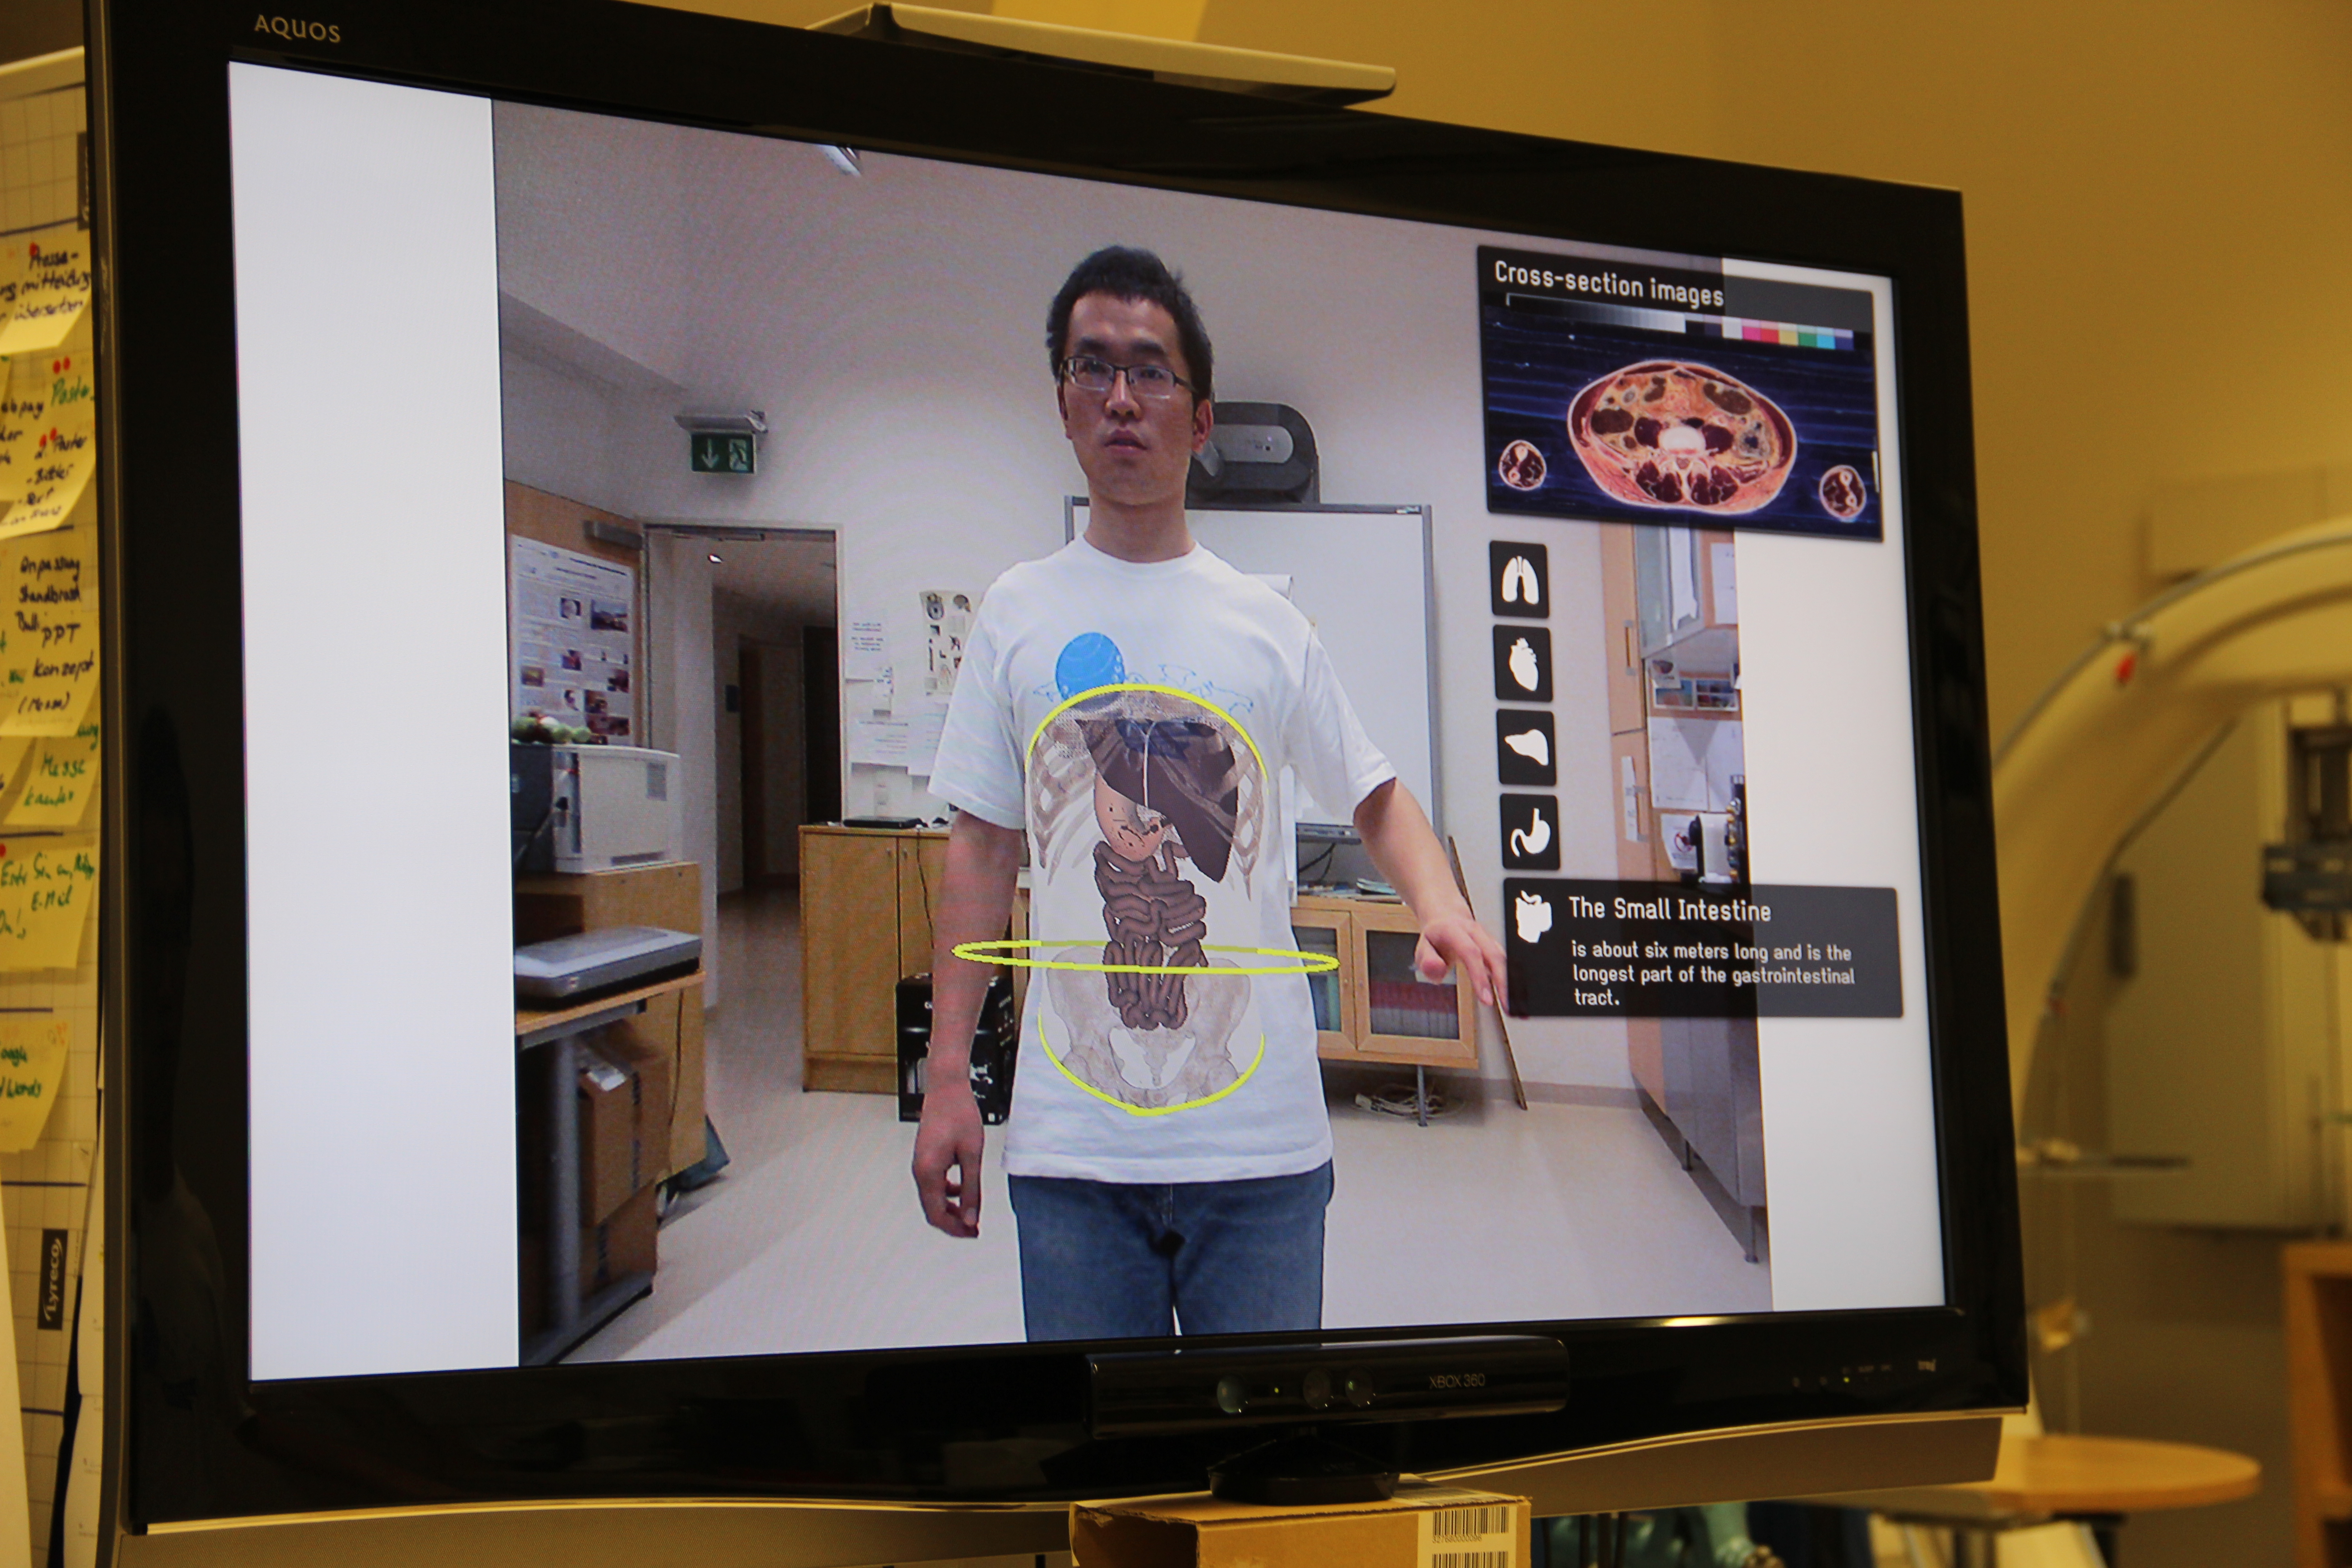
\includegraphics[width = 0.7\linewidth]{figures/3-MMC/Figure1.JPG}
	\label{fig:3-MMC:fingure1}
	\caption{Personalized magic mirror system for anatomy learning. A sensor tracks the user positions in real-time, and contextual in-situ visualization algorithms enable the augmentation of organs and muscles directly onto the user body.}
\end{figure}

\subsection{Natural perception and interaction}
\subsubsection{AR in-situ visualization of human anatomy}
For a personalized visualization of organs we employ the concept of a magic mirror. The camera image is flipped horizontally and shown on the screen such that the user has the impression of standing in front of a mirror. The system tracks all user movements using a depth camera and an algorithm to detect the pose of the user from the depth image. This is realized using the Microsoft Kinect which was originally developed to allow controlling computer games by motion. Then, virtual objects can be added to the image of the real scene. By using the magic mirror metaphor, the user is led to believe that he or she is able to look inside their own body. At the same time, radiological information (CT data and a fully segmented dataset of cross-sectional photographs of the human body) are displayed in real-time \cite{Blum2012}.

Prior to correctly using our AR magic mirror system, the users stand in front of the monitor and we displayed virtual marks near the five bone landmarks. The users are asked to interactively adjust the positions of the five marks to fit their own bone positions. In addition, the exact locations in the VKH CT dataset of the five selected bone landmarks are known. A linear interpolation was executed to estimate the torso point (i.e. a 6th landmark) in the CT volume to improve the overlay. Then the scale factors and transformation matrix were computed to render the anatomical image onto the user’s body. These landmark positions allow the deformation and interpolation of the medical data correctly within the magic mirror and onto the human body, resulting in a more precise augmentation. A user study involving surgeons and anatomy experts confirmed our findings and will be presented in Section 3.
\subsubsection{Natural User interaction}

\subsection{Potential application with magic mirror}
Medical education 
AR rehabilitation 
Patient positioning 

%todo: {Accuracy of Registration} improve the perception of the MR view via accurate registration. Anatomy learning, personal information (gender, age, body shape)
\section{Personal Registration of Magic Mirror}

\subsection{Personal Information}
We augment a personalized visualization of a CT dataset onto the user. However as full CT scans of any user are generally not available, we use the Visible Korean Human dataset (VKH), which consists of a CT scan, an MR volume and a photographic volume which has been acquired by stacking up cry sections. To allow a correct augmentation of the CT data, the gender, age, body size and pose of the user has to be detected. This is performed based on the color image using the OpenBR library \cite{Klontz2013} and the depth image using the NITE skeleton tracking software. The corresponding CT volume is chosen and scaled to the size of the user and augmented onto the user body. For visualization of the bones a transfer function is used as bones can be distinguished easily in the CT volume based on their voxel intensities. For the organs a segmentation of the VKH is used. The augmentation uses contextual in-situ visualization such that the virtual objects are only shown through a circular window. This leads to a better perception of depth, compared to a simple augmentation of the whole CT. The user could naturally turn around their body to check CT volume from different viewpoints and put their right hand at different heights to select a body plane with corresponding anatomy.

\subsection{Personal Registration}
We presents a general method to interactively improve and correct the Kinect skeleton for anatomy education purposes. We believe that our general method can be applied to projectors or other sensors as well for augmented reality. A thorough validation of our method demonstrated improved precision of anatomical landmarks and opens the avenue to future improvements in medical education. Together with the ISMAR community, we hope to initiate such discussions in integrating exciting user-interaction and gaming concepts within our system.

Our AR magic mirror relies on Kinect sensor which offers an imprecise skeleton tracking output (see \figurename{\ref{fig:3-PRMM:bonelandmarker}}). This limits the precision of our magic mirror augmentations offering users false anatomical positions overlaid onto their body, resulting in a poor medical learning environment. Alternatively, had we considered projectors to display human anatomy directly on a user’s body the same inaccuracies would exist\cite{Sun2013}. 
\begin{figure}[htb]
	\centering
	\label{fig:3-PRMM:bonelandmarker}
	\includegraphics[width = 0.75\linewidth]{figures/3-PRMM/FiveBoneLandmarker.png}
	\caption{Selected anatomical points for Kinect skeleton improvement and subsequent CT warping and interpolation.}
\end{figure}

The goal of this method is to propose a more precise user-specific learning environment. Together with orthopedic surgeons we have defined anatomical bone landmarks: (i) which are correctly identified in medical data such as CT and (ii) which users can touch easily on their body while standing in front of any sensor. These landmark positions allow the deformation and interpolation of the medical data correctly within the magic mirror and onto the human body, resulting in a more precise Kinect skeleton and augmentation. A user study involving surgeons and anatomy experts confirm our findings. 

The skeleton output from Kinect limits the precision of the AR magic mirror applications. Thus, our magic mirror augmentations would contain errors and users would easily distinguish anatomical offsets on their body resulting in a poor anatomy learning environment. Alternatively, we had considered projectors to display human anatomy and along with their existing limitations the same inaccuracies would exist. Our aim was then to propose a method to correct for such overlay inaccuracies that could be translated to any magic mirror system worldwide. Together with orthopedic surgeons, we have defined five bone landmarks that (i) users can easily identify and touch while standing in front of the Kinect, and (ii) that are accurately and easily identified in medical data such as CT \cite{ma2013ismar}. These are: left and right acromion, left and right anterior superior iliac spine, and the manubrium (see \figurename{\ref{fig:3-PRMM:5points}}).


\begin{figure}
	\centering
	\subfloat[~Improvement of Kinect skeleton]{
		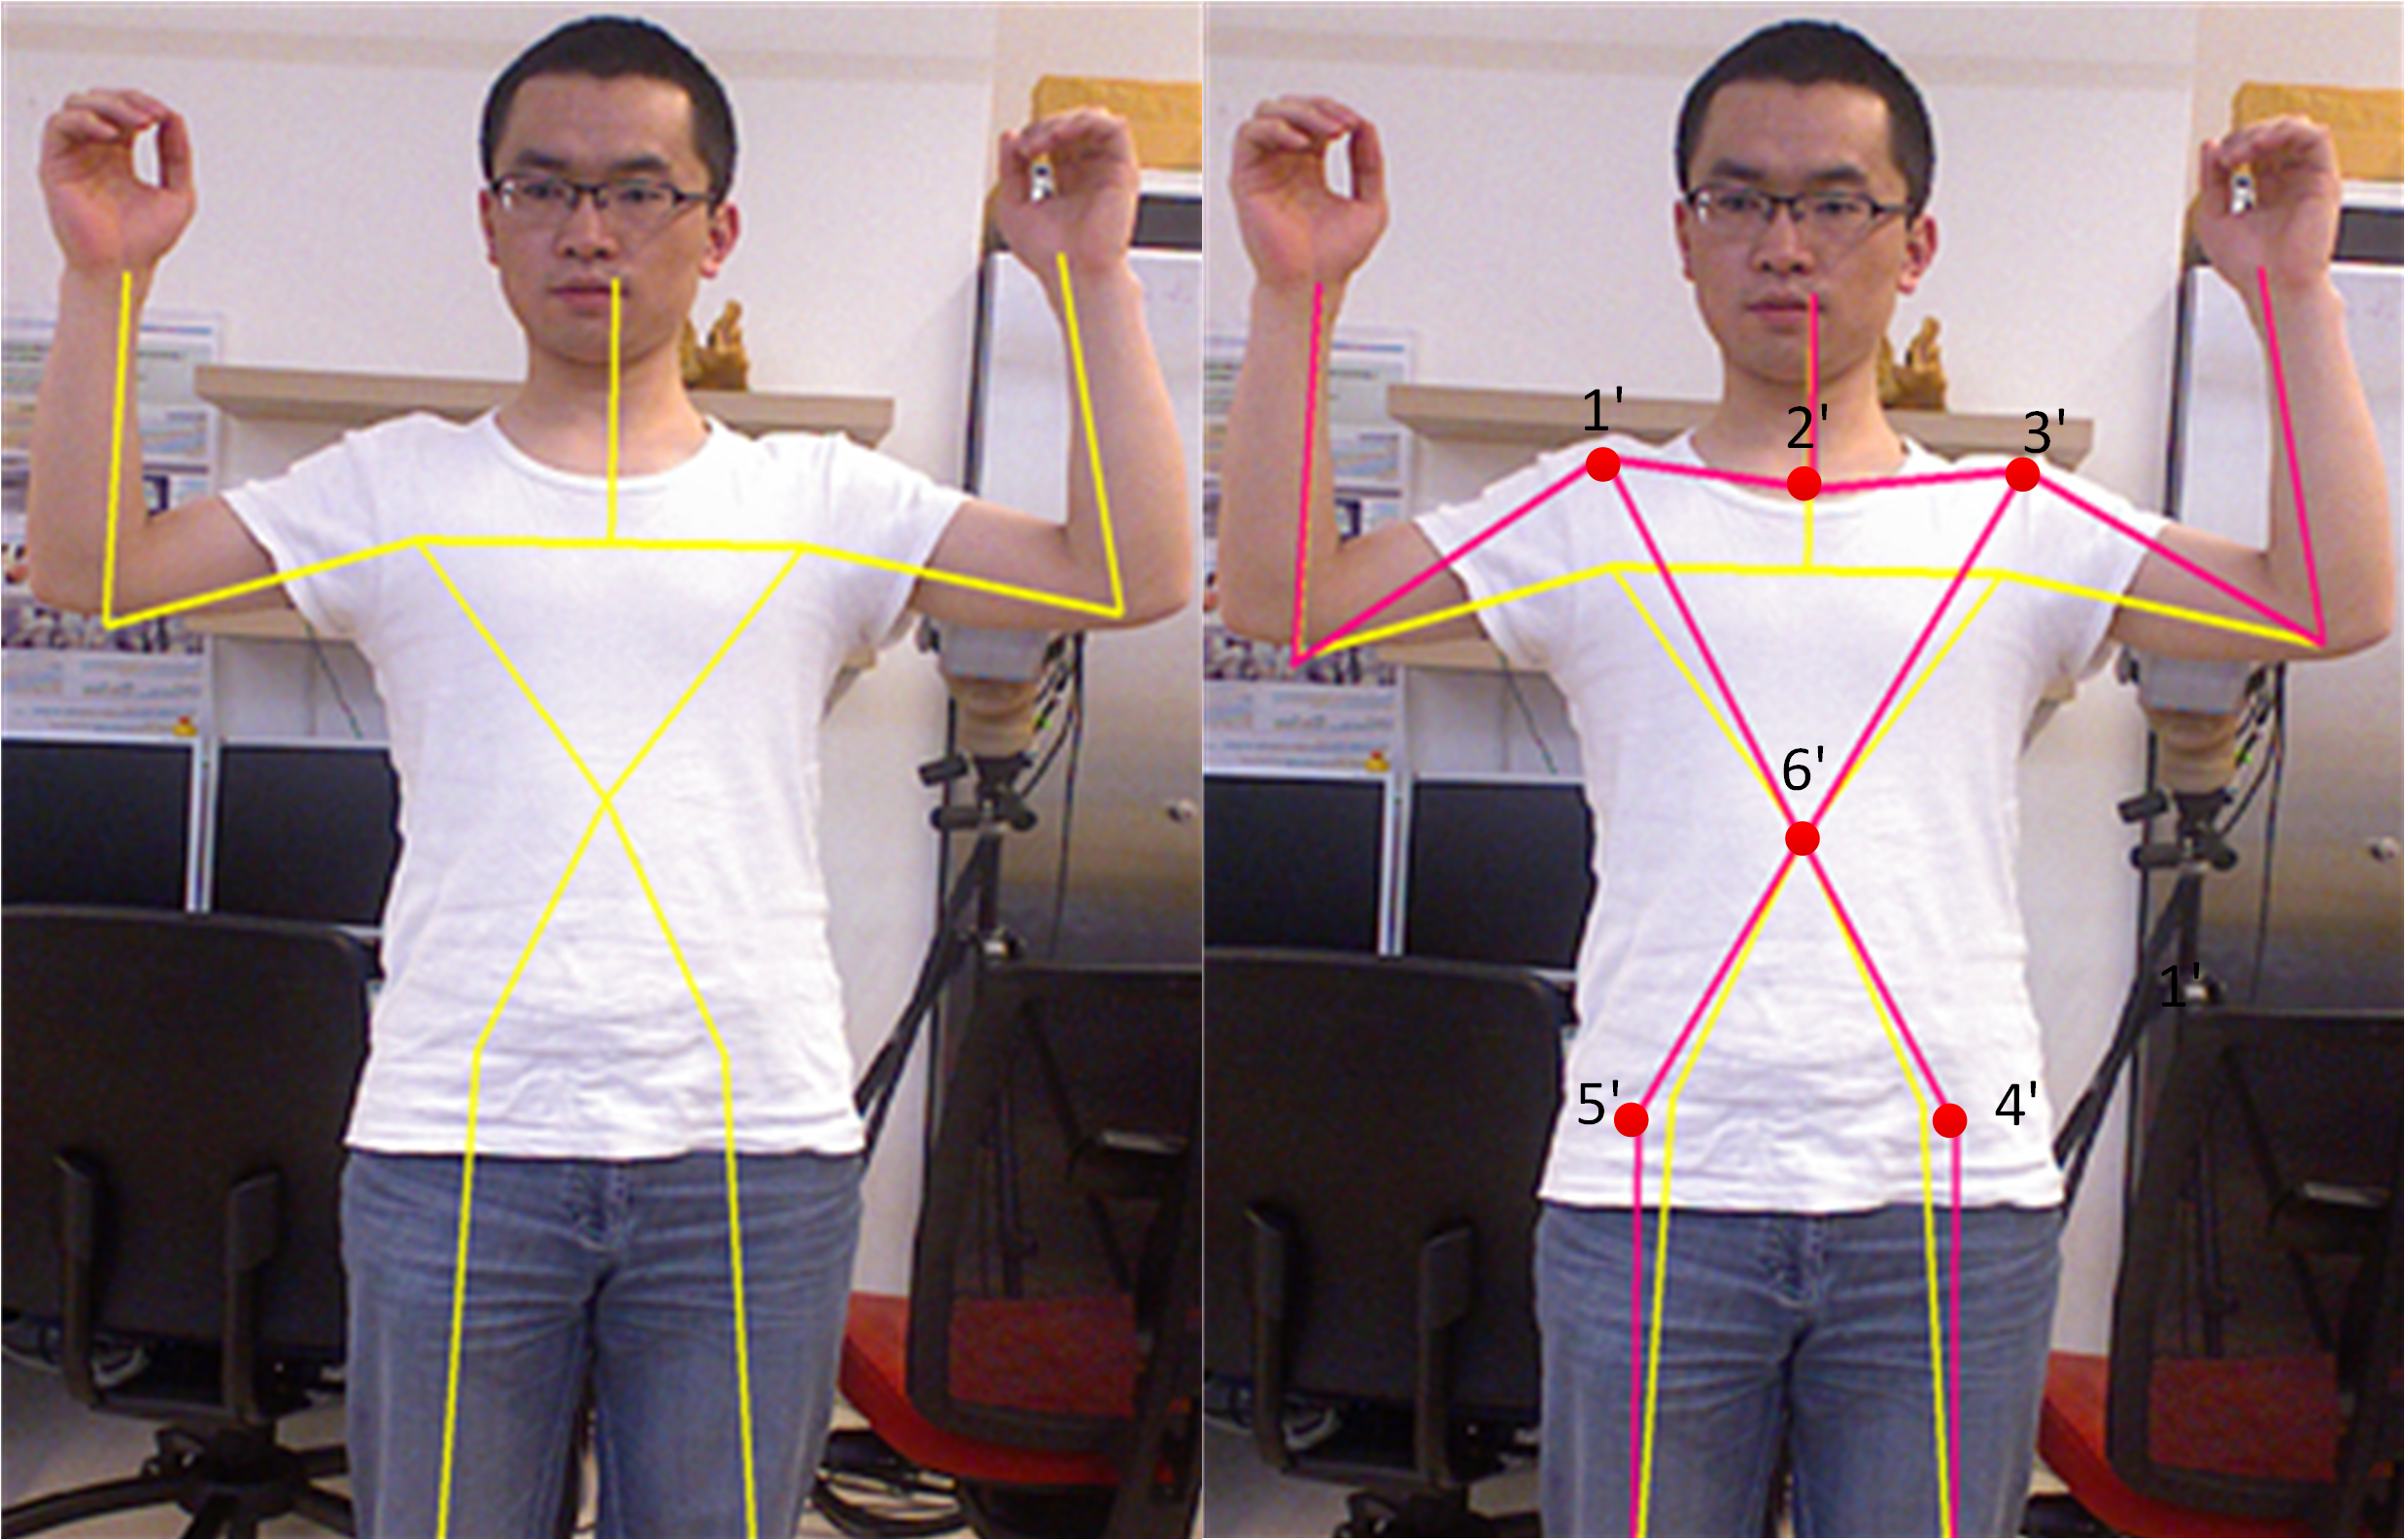
\includegraphics[height = 7cm]{figures/3-PRMM/ModifiedSkeleton.png}
		}
	\quad
	\subfloat[~Bone landmarker in CT volume]{
		\includegraphics[height = 7cm]{figures/3-PRMM/BoneLandmarkerInCT.png}
			}
	\label{fig:3-PRMM:5points}
	\caption{(a-b) The inaccurate Kinect skeleton, in yellow, compared to the improved Kinect skeleton positions in red. (c) CT data from the Visible Human Korean showing the 5 landmarks from Kinect skeleton. (d) CT data showing correctly the 5 landmarks + interpolated torso landmark using our method.}
\end{figure} 
\subsubsection{Anatomical bone landmarkers}
Together with orthopedic surgeons, we have defined five bone landmarks that can easily be touched on the human body. These are: left and right acromion, left and right anterior superior iliac spine, and the manubrium. Subjects are positioned in front of the Kinect sensor and asked to interactively adjust the positions of five landmarks
\subsubsection{Improment of kinect skeleton}
Figure 3 shows a comparison between the traditional Kinect skeleton and its proposed improvement. The first row depicts visually the exactness of the new skeleton. The second row depicts the skeleton landmarks directly on CT data. We observe that the shoulder and anterior superior spine are inaccurate in the images. The last row depicts the improved landmark positions within CT as well. Transverse and sagittal CT slices of the visible human Korean are seen respectively in rows 2 and 3.
In Figure 3a, the following scale factors were computed for the magic mirror augmentation:

\subsubsection{Evaluation}
As an augmented reality anatomy learning application, both accuracy and system usability are very important prior to its translation in classroom. Firstly, we undertook one user study with particular users having expert anatomy knowledge to evaluate if this system is precise enough for anatomy learning. Secondly, another user study involving first year medical students took place to verify the learning potential and acceptability of our technology as a compliment to atlas textbooks in classroom.

\paragraph{Assessing the magic mirror system precision and usability}
Participants: Seven participants were included in this study (two surgeons and five final year undergraduate medical students). 
Analysis: a Likert scale was used which is a type of psychometric response scale often used in surveys and the most widely used scale in survey research. When responding to a Likert questionnaire item, respondents specify their level of agreement to a statement. The format of our 5-pt Likert was: (1) strongly disagree, (2) disagree, (3) neither agree nor disagree, (4) agree, (5) strongly agree. 
To assess the precision of our personalized magic mirror we asked the participants to interact with the system platform which integrates user-specific anatomical landmark selection. Participants were asked to provide an estimated numerical offset, if any, on how far specific bone landmarks or organs were with respect to their own body. For this, they interacted with the magic mirror window, CT data, and used their own medical knowledge and expertise for judgment. CT data was displayed in an interface depicting both transverse and sagittal planes, and participants would quantify the offsets. If needed, a ruler was provided to assist them. The anatomical targets during evaluation were defined as: the anterior superior iliac spine, manubrium, heart, and liver. Results from this exercise are shown in \tablename{\ref{tb:3-PRMM:results1}}, with offsets measured in centimeters. Results from the user study show that the precision of user-specific learning environment is on average 0.96cm.
\begin{table}
	\caption{Precision (in cm) of magic mirror system based on anatomical offsets}
	\label{tb:3-PRMM:results1}
	\scriptsize
	\begin{center}
		\begin{tabular}{p{4cm}|p{3cm}}
			Anatomy & Offset(Mean$\pm$ STDev) \\
			\hline
			anterior superior iliac spine & $0.67\pm0.52$\\
			manubrium & $0.67\pm0.75$ \\
			heart & $1.17\pm1.60$\\
			liver & $1.33\pm1.21$
		\end{tabular}
	\end{center}
\end{table}

The seven participants were then asked to judge the usability of the AR magic mirror system by responding to the following questions: (i) is the overlay accurate w.r.t human body (ii) is the user interface easy to use, (iii) is it fun to play, (iv) can it be used for medical education, and (v) would it have stronger impact for medical education learning?
The Likert scale results for the first four questions are shown in \tablename{tb:3-PRMM:results2}.
\begin{table}
	\caption{Likert scale results regarding magic mirror usability}
	\label{tb:3-PRMM:results2}
	\scriptsize
	\begin{center}
		\begin{tabular}{p{6cm}|p{3cm}}
			\space & Mean$\pm$ STDev \\
			\hline
			is the augmented reality overlay accurate w.r.t human body & $4.00\pm0.89$\\
			is the user interface easy to use & $3.67\pm1.03$ \\
			is it fun to play & $4.50\pm0.55$\\
			can it be used for medical education & $4.17\pm0.75$
		\end{tabular}
	\end{center}
\end{table}
For the last question regarding the impact of our technology, there was a unanimous response that the AR magic mirror system should be considered as a potential platform to complement existing anatomy learning tools inside anatomy classrooms. 
\subsubsection{Discussion}
The precision of our method is visually demonstrated in Figure 3c-d and \figurename{\ref{fig:3-PRMM:ResComparing}}. We observe that the acromion and anterior superior iliac spine, using the traditional Kinect skeleton, is not positioned correctly within the CT data compared to the modified Kinect skeleton version (1-2 vs. 1'-2'; 3-4 vs. 3'-4'). The orthopedic surgeons participating in our study confirmed this.
\begin{figure}
	\centering
	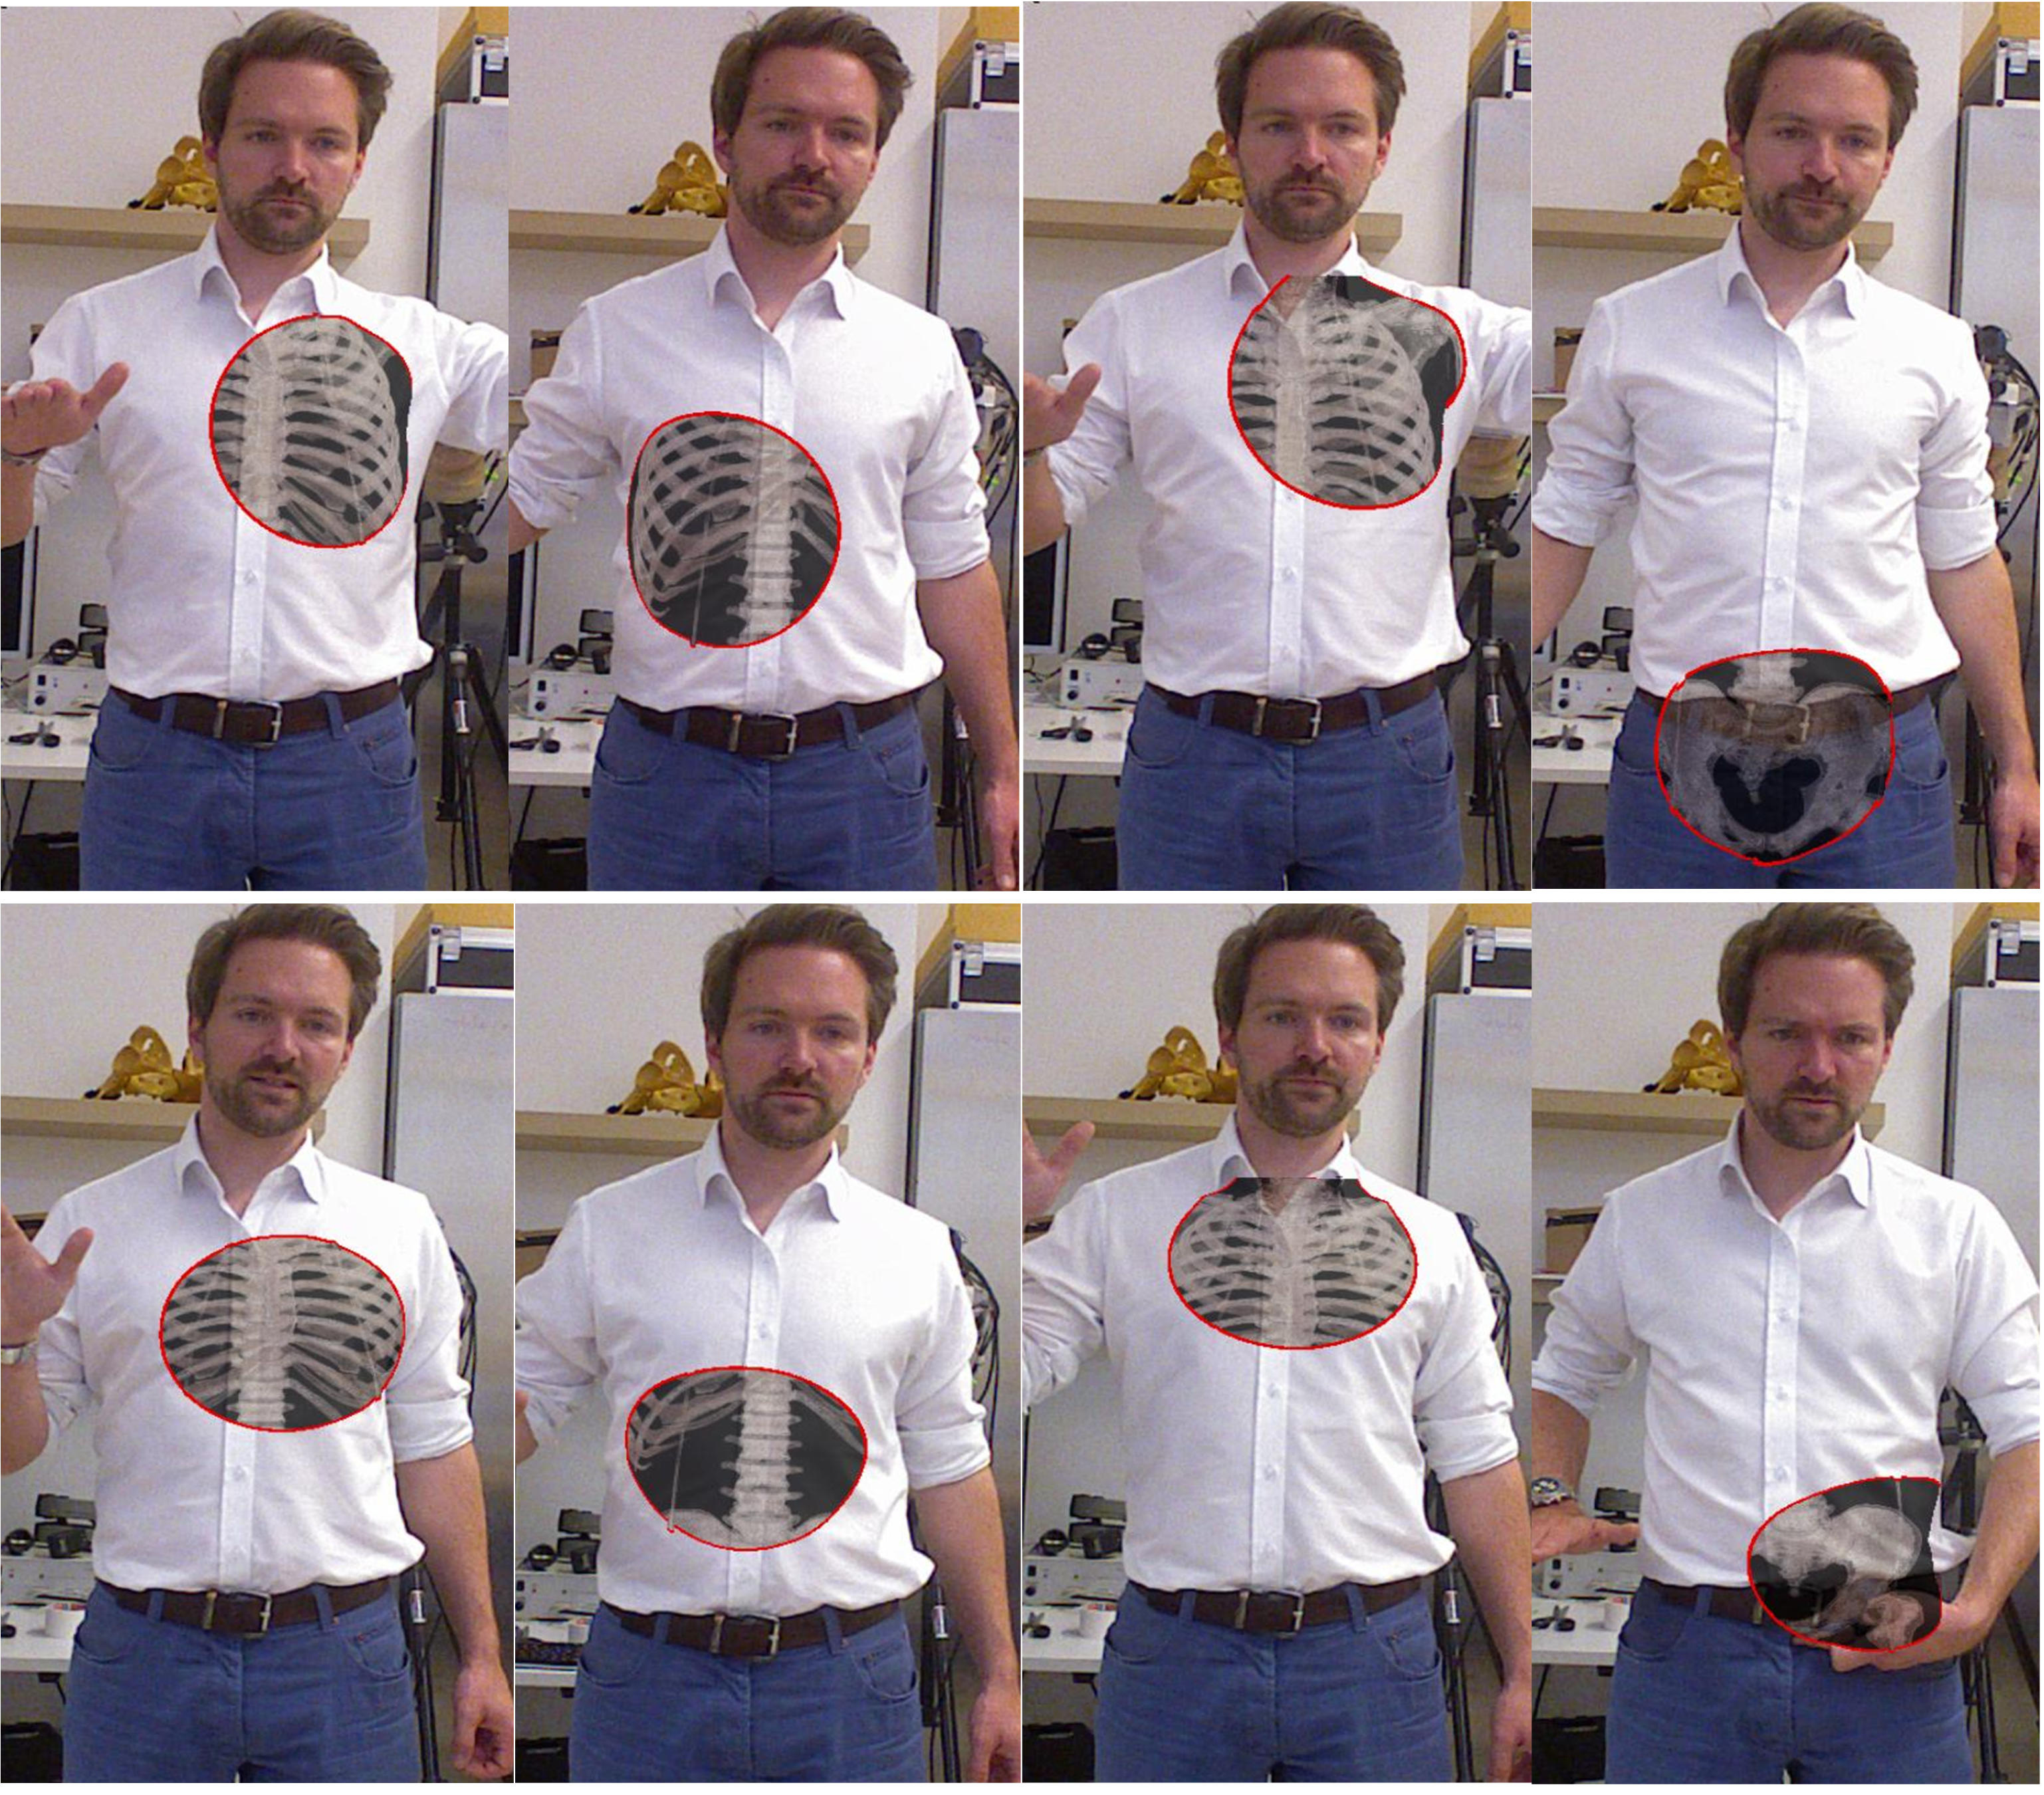
\includegraphics[width = \linewidth]{figures/3-PRMM/ResComparing.png}
	\label{fig:3-PRMM:ResComparing}
	\caption{Figure 4:	The magic mirror before (top) and after (bottom) the Kinect skeleton adjustment. Column 2 depicts the bottom of the rib cage being positioned correctly after skeleton correction.}
\end{figure}
Results from a user study show the impact of interactively improving the Kinect skeleton to increase precision for a better visualization of anatomy. The offsets of specific anatomical landmarks decreased significantly. The following comments were collected:
\begin{enumerate}
	\item the precision improved; making the user touch anatomical landmarks is cool since this is the way it is done in clinic…
	\item two additional landmarks easily accessible are the sternum and bottom of rib cage…
	\item make the magic mirror circle bigger for larger anatomy…
	\item voice command is a good idea but it is sensitive to the surroundings voice
	\item interactions between observers …
	\item could introduce the female CT visible human Korean…
	\item could use a healthy patient CT or other modality…
	\item could make the CT slices bigger on the screen…
\end{enumerate}

One appealing feature of the system is that with the Kinect we are using inexpensive standard hardware. In the future such a system could be made available to students or patients who have to do rehabilitation exercises at home. In addition to the full system using a large screen and a screen stand we also want to evaluate the benefit of making the system accessible to students when they are at home and at any time. We want to do this for two different reasons. First, there is a trend toward competency-based education in medicine. Instead of defining a curriculum, learning outcomes are defined. Students have to fulfill these learning outcomes. The advantage of competency-based education is that all students will have the same competency in the end. A student who is less skilled has to take more time to learn than a student who already has good skills. One requirement for this is that the students have to be able to educate themselves until they reach the required competency. We plan to use the AR magic mirror system both to allow them to do training and to test whether a learning outcome has been met. The magic mirror has to be made easily available to them so that they can use it for training at any time. The second reason to develop a distributed system which can easily be used by students is to collect user statistics.

Many medical education systems are web-based and allow accessing them from every computer. However current systems do not use high-end visualization and input devices like the Kinect. In the future when technologies like HTML5 and WebGL have matured it can be imagined that a system like the magic mirror could be implemented using web technology such that it can run on any computer. However, at the moment the use of web technology would be a significant limitation. We are using very large datasets, high-end visualization, GPU computing and gesture-based interaction.

It was originally suggested to us that our system would have much more of an impact for medical education learning if it were to be translated today in medical schools and anatomy classrooms. As such, with the help of our co-author and anatomy professor, we deliver the improved AR magic mirror to two anatomy classes within the Anatomy Department of the Ludwig Maximilian University (LMU) Medical School, Munich, Germany. The anatomy professors made it clear that the AR magic mirror system is exciting, but has to go beyond state-of-the-art technology to be truly useful for education. Our participants stressed the importance of visualization of anatomy that can change dynamically resulting from the actions of the user moving the body, and also for visualization of muscles. Furthermore, more advanced user interactions like the use of gaming elements would be required to make the use of the system for learning tasks more interesting.
% !TEX root = ../thesis-example.tex

%todo: Make the user believe the virtual element is a part of his or her own body. (Organ game and the Muscle learning)
\section{Interactive Mixed Reality and Serious Gaming} \label{sec:3-PPMM:IMR}
%Personalized natural interaction \& gaming
Although we can lean by reading and watching and real depth of understanding, the learner always needs to encode the knowledge herself, rather than simply receive what is shown. This is one of the reasons that interacting with the mixed reality system can be a powerful learning tool - we are not only get the benefit of AR view, but also receiving immediate feedback. Knowledge is a process of understanding by connecting. These interactions are often useful in creating the aha moment -- the joining of medical knowledge with a learner's own body and movement.
In last section, user's personal information was collected to improve the general perception of the medical information.
Here, we tried to implement several applications in integrating exciting user-interaction and gaming concepts within the proposed magic mirror framework.
 
%Two kinds: user motivate interaction (user's movement trigger the changing) and scenario interaction (AR view change according to the presetting), combine two kinds together. 
The basic magic mirror system focuses on the abdomen organs as real-time deformation of the 3D medical images is very difficult. Firstly, we extent the magic mirror to visualize the basic function of the human skeleton and muscle system, since each bone of the skeleton system is also a rigid object and is controlled by muscles via attachment points. Besides mirroring the users movements to the skeleton, the system  also visualizes active muscles and implement a labeling system, which can be used to show the names of the muscles or bones.
Then, a new interaction with anatomy is developed for learning in the augmented reality magic mirror framework. It allows the implementation of independent modules on top of mirracle, which is demonstrated by the two modules for the organ atlas and the education game that are already taking advantage of this infrastructure. The organ atlas is a good way of imparting anatomical knowledge on the users, allowing them to explore their body without any instructor or supervisor.
The interaction methods we developed are not necessarily limited to self-referenced selection and manipulation. In general cases, they are suitable for scenarios where many possible items are densely packed and a user wants to select a single or multiple items in an augmented or mixed reality environment. The large number of possible modifications to the methods make them difficult to configure, but the general ideas should be applicable to many use cases.
Thirdly, Figure 4 depicts the visualization of muscle anatomy of a human arm. The magic mirror was embraced by the majority of the medical students in its current version. Based on our discussion with them we found that the students really liked the AR visualization on their own bodies, however they were not used to the natural user interface and gestures required for interaction. A learning curve was necessary for them to appease initial frustrations they had when first using our system.
Finally, serious gaming for education and rehabilitation is discussed. One education game is developed taking advantage of the new interaction method with the anatomy, and a AR knee rehabilitation demo is developed. 

\subsection{musculoskeletal Animation} \label{sec:3-IMR:musculoskeletal}
Instead of rendering the bones from a rigid CT dataset, a polygonal model will be used to create the AR view of the skeleton. Then, we can animate the model based on the orientation of the joints received from the skeleton stream to match the pose of the user in front of the system.
The objective of this application is to develop a simple non-physical visual effect of the musculoskeletal system based on models from OpenSim\footnote{\url{https://simtk.org/home/opensim}}, which is freely available, user extensible software system that lets users develop models of musculoskeletal structures and create dynamic simulations of movement. Besides mirroring the users movements to the skeleton, the system also visualizes the relationship between bones and muscles. Furthermore, a labeling system is implemented which can be used to teach the user names of the muscles or bones (see \figurename{\ref{fig:3-IMR:skeletonMuscleDemo}}).

\begin{figure}
	\centering
	\includegraphics[width=0.7\linewidth]{figures/3-IMR/skeleton_Muscle2.png}
	\caption{Musculoskeletal Animation in magic mirror: an application to show a simple non-physical visual effect of the musculoskeletal system based on models from OpenSim}
	\label{fig:3-IMR:skeletonMuscleDemo}
\end{figure}

\subsubsection{OpenSim Musculoskeletal Model}
OpenSim is an open source software platform for biomechanical modeling, simulation, and analysis. The GUI includes many tools for loading data, creating and editing models, visualization of the simulation results, and much more. The API allows programmers to access the core components of OpenSim to create new plug-ins for the GUI or take advantage from it in theirs own applications. It also includes some validated musculoskeletal models and more can be downloaded from the platform website\footnote{\url{www.simtk.org}} where researchers can provide their work \cite{Delp2007}.

OpenSim Musculoskeletal Models consist of bodies, joints, forces, constraints, controllers, markers, and contact geometry (see \figurename{\ref{fig:3-IMR:openSimModel}}). The skeleton is build up with rigid bodies and joints connecting two bodies. A body has attributes for its mass, center of mass, and inertia. It can include display geometry for bones. Joints have an attribute for their position in the parent body and hold a joint type dependent transformation to define the motion of a body relative to its parent body. Movements can be further restricted by constraints. Muscles are modeled as forces that are exerted on attachment points to the rigid bodies. The force of the muscle is dependent on its path (through all the attachment points) and muscle properties like maximum force, optimal fiber length, tendon slack length, pennation angle, and maximum contraction velocity. 
From the OpenSim models, we can definitely use the skeleton model and the paths of the muscles, by a conversion of the geometry data and reorganization of the scene graph. But, the muscle states simulation functions are difficult to integrate into magic mirror system, since it can not calculate the muscle activity in real time.
\begin{figure}
	\centering
	\includegraphics[width=0.8\linewidth]{figures/3-IMR/openSimModel.png}
	\caption{OpenSim Musculoskeletal Model: The skeleton is build up with rigid bodies and joints connecting two bodies. Muscles are modeled as forces that are exerted on attachment points to the rigid bodies. }
	\label{fig:3-IMR:openSimModel}
\end{figure}

\subsubsection{Application Design}
Based on the magic mirror framework, the application is designed according to the following rules. The objective is a simple interactive MR application for education.
\begin{itemize}
	\item Accurate AR view of the skeleton.
	\item Clear relationship between the bones and muscles.
	\item Estimate the muscle active states when the user performs movements.
	\item Highlight the active muscle according to the movements.
	\item Information of the bones and muscles for learning.
\end{itemize}
A general musculoskeletal model is created according to the OpenSim models and it contains the bone geometry, connections between the bones, muscles and attachment points to the bones. Skeleton and muscles are load to the application as two separated sub scene graphs, as  the skeleton model can be used independently for many purposes. In real world, the muscles control the bone movements, but the muscle model is dependent of the skeleton model in the application as the system input are just the positions and orientations of the skeleton joints. The skeleton model is transformed based on the skeleton stream from the Kinect and the muscle model is then updated as it is affixed on the bones via the attachment points. Both models are rendered to create the non-physical visual effect to generate the AR view. 

\paragraph{Update Skeleton Model}
After a user is calibrated, the skeleton model is scaled to fit the current body. The proportion of the user can be estimated through the pose matrices. The scale method first scales the root node which is the pelvis and it actually scales the whole model. 
The scale factor is calculated from the distance of the right shoulder to the left hip. So this scale factors represents the average of width and height of the torso relative to the general model. In practice using this approximation gave better results then calculating two different scale factors. 
The accuracy of the proportions of the legs could be improved by calculating the distances between hip, knee, and ankle. We employ the same scale as the torso when the knees and ankles are not observed by the sensor.
Here we also define a calibration pose to get an accurate measurement of the segment length. 
The calculation of the transformation of each joint on the model is also another important task. The relationship between the coordinates spaces of Kinect, OpenGL, and the skeleton model has to be carefully analyzed. In order to obtain the correct relative rotation of each bone, quite a few transformations have to be apply to the raw joint orientation from skeleton stream. The skeleton model is then animated to mirror the body movements.

\paragraph{Update Muscle model}
The muscle model contains all the individual muscles, which is displayed in the application. Each muscle is model as a 3D string which goes through all the attachment points. So the muscle model is dependent of the skeleton model and is first created based on the general skeleton model. Wherever the skeleton model is updated, each muscle model is also recreated to make sure the size and special relationship is correct. 

%add an attachment point to define the path of each muscle model 
The attachment point information for each muscle is textually found inside the OpenSim 'osim' model file. Each attachment point is defined by the bone's name, 3D position in the bone coordinate system, and the type of point. One muscle has several attachment points, which define the relationship with the bones. A xml file is create to save all muscle information.
In the application, 3D strings are rendered between each pair adjacent attachment points. 
The color of the string is defined as the active state of the muscle and the line width can be adjust according to the muscle's size. The muscle model is not hierarchical as the skeleton model. Muscles are attached to bones in different coordinate systems. As the attachment point is defined in the bone coordinate system, the positions have to be converted to the world space. The world position of the bone is easily calculated by accumulating all the transformations from the skeleton root to the current bone object. Then, each attachment point can be converted to the world space.

A Label class is designed to show text information of the bones and muscles. The Label is meant to display text attached by an arrow to a point in the scene. The special feature of this class is that two labels will never overlap. The originating point of each label is from the object, e.g., a bone or a muscle, and where the text is actually drawn depends on the sorted vector of the all visible labels. The text is drawn always below the text of the label previous and connected with a line to the originating point (see \figurename{\ref{fig:3-IMR:openSimModel}}).

%update muscle color 
When a new frame comes in, the system updates the skeleton model according to the orientation of the each joint. And the world coordinates of each bone and attachment points are calculated. The length of each muscle can be estimated by the distances between the points. The active state of the muscle can be simple assessed based on the length change. A muscle is active when its lengths is shorter than the initial length or at least shorter than its previous length.  In this case the color will be scaled between red and green dependent on the difference. Red means that the muscle is active and green means that the muscle is approximately inactive. It depends on the contraction speed and the length of the muscle. This method does not compute forces like OpenSim, it only estimates the activeness of the muscle very coarsely. Finally, muscles are redrawn with the new position and new color.

OpenSim provides some advanced function to simulate the active states of the each muscle based on the body movement, but the approximation in real time is not possible right now and only the skeleton position stream is too noisy for such simulation. Another possible solution to fetch more accurate muscle state is to attach electromyographic sensors onto the user's body. This should be one of the future work for this thesis. 
%In the next step the color of the muscle is recalculated.
%The color is going have a portion of green of intensity and a portion of blue of 1-intensity. The intensity is defined as the square difference of the length and previous length of the muscle normalize by the initial length. So the intensity is influenced by the speed of the contraction. If the length of the muscle is shorter than the initial length then one can average it with intensity2 for the actual amount of contraction to simulate gravity.The formula for intensity  is obtained experimentally.
%If the muscle is active this is calculation of the color:
%\begin{figure}
%\centering
%\includegraphics[width=0.7\linewidth]{figures/3-IMR/mulcleActiveColor}
%\caption{To calculate the muscle active state and the color mapping function}
%\label{fig:3-IMP:mulcleActiveColor}
%\end{figure}

\subsection{Interaction for Anatomy Learning} \label{sec:3-IMR:anatomyLearning}
Basic Knowledge of human anatomy is not only important for medical doctors or health-care professionals, it is also considered common knowledge that is taught at various levels of school education. To improve the conventional book-based methods for anatomical education, we investigate the suitability of an augmented reality system using a magic mirror metaphor for this task.
With the existing platform serving as a basis, we first have developed an abstraction framework offering a general interaction for augmented-reality applications. On top of this framework, we have implemented an interactive educational application consisting of an organ atlas and a complementary organ learning game, leveraging the benefits of self-referential learning and motivation through game challenges.
%To achieve intuitive usability, we investigate different user interaction methods for organ selection in a self-referential system using augmented reality, providing methods for unique selection as well as coarse, non-unique selection.
\paragraph{Interaction Challenge}
The most challenging problem of the idea turned out to be the selection and interaction methods with the organ model. For our idea to work, we need a method to reliably detect which organ the user has selected while leveraging the mirror analogy as far as possible. The most intuitive and direct way would be to use a virtual hand technique to directly select the organs \cite{Ha2010}. This, however, is bound to fail for two reasons:
First and most obviously, it is not possible for the user to put his hand into his body and directly touch the organ, he is merely able to point to the approximate region in front of the organ. This region he is able to indicate is not accurate and in many cases it is not really possible to detect reliably which organ the user meant. Especially in the abdominal area many organs are fit very tightly together in one place, making it very hard to distinguish between two organs.
Secondly, the tracking capabilities of the current version of Kinect sensor used in our implementation are somewhat limited. The only thing suitable for selection that is reliably tracked is the position of the hands. Neither orientation of the hand nor information about the fingers is available. This makes it even harder to develop a suitable, intuitive interface. Untrained users usually use their fingers when asked to indicate a point, but since we can only track the hand position, there is always an offset to our tracked position and the position the user was actually indicating, and this offset is not static but depends on the hand orientation and size and position of the fingers we know nothing about.

\subsubsection{Motivation and Objective}
To provide an alternative method for medical teaching, we have developed a computer-based system allowing the users to have a virtual look into their body. We use the magic mirror concept as a basis for our augmented reality application: The users can see themselves on the screen like in a mirror, but with additional information like computer models of their inner organs augmented onto his body. Here, we try to expand this existing implementation to be used as an alternative and entertaining way to teach human anatomy. A general framework to support generic extensions of the magic mirror system is first implemented. Using this framework, we implement an educational application, an interactive organ atlas to allow the user to explore his body and learn about spatial relations, visual appearance and function of the organs. An organ learning game to provide an entertaining way to learn anatomy is also presented in section \ref{sec:3-IMR:gaming}. This game is based on the knowledge presented in the atlas and leverages augmented reality and motivation through game challenges to improve the learning performance of the user. To achieve this goal, we examine different interaction metaphors and their suitability for the tasks presented.

In the AR learning environment, organ selection is a challenging task as some organs hide behind others. The user cannot directly position their hand into their bodies and to select the organ of choice. In engineering design, mechanical parts are drawn with the innermost part at the center, while the others are moved some fixed distance outwards to display all parts of the assembly that would otherwise be hidden. Inspired by this principle we designed and developed an organ explosion effect (see \figurename{\ref{fig:3-IMR:organExplosion}} ), which separates the organs. The organ explosion selection employs a two-hand interaction method. Using the left hand, the user is able to focus the height for the section they are interested in. Organs at approximately the same height are then projected outwards. Using a spherical projection, the organs are moved outward, creating the illusion of seeing them `fly out' in front of the body. Lines are drawn to indicate the original position of the organs. After separating the organs from each other, it is easy for the user to select the organ of interest using their right hand. Another functionality of the organ explosion effect is allowing the user to rotate and observe the 3D organ models and perceive the spatial relationship between them.

We implement an interactive anatomy atlas that is, in our first prototype, limited to the inner organs of the torso. The user can explore these organs and read additional information on each of the visualized organs. The work is separated into two different parts: A general framework performing all kinds of basic operations not specific to any application and the actual application logic implementation and realizing the organ atlas application.
The general interaction framework is designed to be an abstraction layer on the magic mirror framework and provides easy access to implement custom application logic, making it easier to experiment with new ideas based on the magic mirror system.

\subsubsection{System framework}
The main design goal is that abstraction is extensibility, to encapsulate all the interaction and visualization functions behind the application logic layer. Hence,  it is very easy to implement new games and other applications or experiments using the offered interaction interface.
The requirement is the possibility to develop different applications based on the framework and allowing integrating them into one single application with as little effort as possible. 

The investigation of possible interaction methods forms an important part of this work. Since conventional point-and-click selection methods are only of limited use for self-referential selection in AR environments, we have developed new methods better suited for our use case: One is driven by a two-handed interaction method to allow the user to select the region of interest with one hand and using the other hand to select a specific organ; The other uses a single-handed approach where the user indicates the organ directly by touching the specific region of his anterior torso. The system then detects possible selections and thus does not provide a single, unique selection in most cases.

\paragraph{organ Explosion}
Our approach to overcome the selection challenge is a technique that we, have called ``Organ Explosion" effect (see \figurename{\ref{fig:3-IMR:organExplosion}}). This technique is inspired by exploded view drawings known from engineering, where the goal is to depict how mechanical parts are to be assembled. Usually they are drawn with the innermost part at the center while the other parts are moved some fixed distance outwards to display all parts of the assembly that would otherwise be hidden.
We use the same basic idea in our interaction technique by implementing a two-handed interaction method: Using the left hand, the user is able to set the focus height for the region he is interested in. Organs at approximately the same height are then projected outwards. Because we use a spherical projection with the center at the height of the hand, but at a point behind the body, the organs are moved outwards, creating the illusion of seeing them fly in front of the body. This way we are able to separate the organs close together since organs at different angles to the projection point are projected into different regions. We scale the magnitude of the displacement down with the distance between hand and body to allow the user to see the organs in their original arrangement but still enable him to ``zoom in" for detail and selection. \figurename{\ref{fig:3-IMR:organExplosion:b}} depicts how this technique looks in practice.
Once we are able to separate the organs from each other, it is easy to check for selections using a direct mapping from the physical right hand to the virtual one and just checking for intersections between the hand and the organs.
\begin{figure}
	\caption[Organ Explosion]{Left: Quantities involved in the calculation of the position offsets for the technique (organs not displayed). In this image, four organs are displaced. Purple dots are original organ positions, blue dots displaced organ positions. The Yellow dot signifies the projection center. Right: Screenshot of the explosion technique.}
	\label{fig:3-IMR:organExplosion}
	\subfloat[Front View] {\label{fig:3-IMR:organExplosion:a} 
		\includegraphics[height= 7cm]{figures/3-IMR/organExplosion2}}
	\subfloat[Side View] {\label{fig:3-IMR:organExplosion:b} 
		\includegraphics[height= 7cm]{figures/3-IMR/organExplosion1}}
\end{figure}

\paragraph{Interaction test for Selection}
Intersection detection between different 3D objects is a built-in functionality in rendering library. A virtual predefined sphere or cylinder is attached to control hand of the current user. The selection function is triggered when the intersection test between the hand object and the organ models. 
For performance reasons, we only use bounding-box intersection tests and skip the narrow phase, treating intersecting bounding-boxes as intersections between geometry. This obviously reduces the accuracy of bounding box tests, this coarse intersection check is better not only in performance, but also from a usability perspective. Intersection tests in our applications are used for checking intersections of the hands with organs. Due to the inaccurate tracking of the hands by Kinect, this actually works quite good when just checking for ``roughly" intersecting pairs.

To further improve performance, we introduce an explicit vector that describes objects that are actually interested in intersections with other objects. The assumption is that general intersections, for example between two organs, are not of interest, while intersections with special objects like a sphere attached to the user's hand are interesting and important.
Once an ``interesting" intersection has been determined between a pair of objects, the first object gets added to the intersecting objects list of the second and vice-versa. This list can then be used and analyzed in the behavior implementation to perform reactions to the collisions.
For convenience reasons, there are two vectors configured to be attached to the left and right hand. They can be added to the framework if required and reconfigured by the application implementation.

\subsubsection{Organ Atlas Application} spatial ralationship and 3D information of the model 
An organ atlas is usually a collection of visual representations of organs or specific organ systems, annotated with names and further information.
We tried to reproduce a version of this concept using our magic mirror framework to implement this idea interactive. The main educational goal of this application is to allow the user to explore the organs of his body and learn about the position, function and spatial relations to the other organs.
We approach this goal by augmenting all available organs onto the user's body and letting him select the one he is interested in. Once the user has selected an organ, the application displays textual information about the organ. This information includes the common, latin and/or greek names as well as a description of the basic purpose of the organ. During the selection procedure, the spatial knowledge of this organ is also learned. If applicable, the organ system it belongs to is mentioned as well as the principle organs it interacts with. An example of what the application looks like in action and finished is shown in \figurename{\ref{fig:3-IMR:OrganAtlas}}.
\begin{figure}
\centering
\subfloat [In action] {\label{fig:3-IMR:OrganAtlas:a} 
	\includegraphics[width = 0.5\linewidth]{figures/3-IMR/FrontViewOrganExplosion}}
\subfloat [Finished] {\label{fig:3-IMR:OrganAtlas:b} 
	\includegraphics[width = 0.5\linewidth]{figures/3-IMR/OrganAtlas}}
\caption{Organ Atlas implementation. Lungs are selected and the infobox shows textbook knowledge about them.}
\label{fig:3-IMR:OrganAtlas}
\end{figure}

The organ atlas described above together with the described exploration and optimized selection methods, offers an interesting new way to explore the human anatomy. However, the described methods offer much room for experiments and improvement. The optimal choice of all parameter values is a very delicate matter that has not been explored fully in this work. The values chosen on an empirical basis seem ``good enough" to at least show that the methods work reasonably well to be used productively. To determine a better parameter, one should conduct a separate study and compare the performance results to generate the parameter settings according to the personal information of the untrained users. Also, the different variations of the methods offer even more room for fine-tuning the effectiveness of this method. 
The organ learning game in its current prototype version already provides a fun experience, but it lacks the content to be distributed as a full game. This could easily be changed by adding more game modes for other organ systems, multi-player modes or other elements commonly found in games.
 
\subsection{Interactive Muscle learning}
Muscles is one very important and difficult topic for all the medical students (see \figurename{\ref{fig:3-IMR:armAnatomy}}). The visual details of the muscle is not presented in the section \ref{sec:3-IMR:musculoskeletal} and functions of the muscle is not easy to learned from the static atlas.  
To evaluate the learning effect of magic mirror, another application framework is developed for muscle learning, currently focusing on the main muscles of one arm related to four basic movements, \textit{flexion}, \textit{extension}, \textit{pronation}, and \textit{supination}. 
The learning targets are the main muscles, which expand and contract during the above movements (see \tablename{\ref{tb:3-IMR:motionMuscles}}).
\begin{figure}
	\centering
	\subfloat{
		\includegraphics[width=0.35\linewidth]{figures/3-IMR/armAnatomy1}
	}
	\subfloat{
		\includegraphics[width=0.35\linewidth]{figures/3-IMR/armAnatomy2}
	}
	\caption{Anatomy of the arm}
	\label{fig:3-IMR:armAnatomy}
\end{figure}
\begin{table}
	\caption[Muscles involved]{The selected motion of one arm and the corresponding muscles}
	\centering
	\label{tb:3-IMR:motionMuscles}
	\scriptsize
	\begin{center}
		\begin{tabular}{|c|c|}
			\hline
			Motion & Muscles \\
			\hline
			\multirow{2}{*}{Flexion} & M.biceps brachii \\
			& M.brachialis \\
			\hline
			\multirow{2}{*}{Extension} & M.triceps brachii \\
			& M.anconeus \\
			\hline
			\multirow{2}{*}{Pronation} & M.pronator teres \\
			& M.pronator quadratus \\
			\hline
			Supination &M.supinator \\
			\hline
		\end{tabular}
	\end{center}
\end{table}

\paragraph{Motivation}
The main objective of the application is to enable the user to acquire knowledge about the bones and muscles of the arm, connecting the procedure with their own arm movement. Based on the magic mirror framework, the non-physical visual effect is the activities of the muscles and the bones. A virtual model of an arm is rendered according to the real arm movement and the AR view is generated.

\paragraph{Application Design}
The application should contain an AR view, which shows the complete color image from the Kinect with the augmented virtual arm. This view acts as the mirror effect and help the user to map all the activities of the bones and muscles onto his/her own arm. Aside from this AR view, there is another virtual view which is program controlled. The virtual view concentrates on the upper or lower arm, showing the details of the muscle model. To preserve the connection between the user and the virtual arm, the AR-view is shown on the left side of the screen after the user is calibrated. The arm model in virtual view only follows the relevant motions, i.e. flexion, extension, pronation and supination. 
The learning patterns include muscle oriented, muscle is displayed one by one, and motion oriented, the user performs the target motions and only the muscles related the current motion is shown. 
We also have to make sure the user can observe the muscle model from different view to learn the spatial information and the learning flow is smooth and friendly. 

\subsubsection{Dynamical muscle model}
\paragraph{Skeleton information}
The position and rotation of the skeleton model are defined in a strict hierarchical order, starting with the spine. The position data from Kinect skeleton stream is in the world coordinate system. To animate the arm model, the relative orientations have to be calculated based on the position of the joints. Only the spine position is directly set as the root's position in the AR view. 
The lower arm is treated separately to the other bone chains. Each hand's orientation is defined using the vectors from the wrist to the tip of the hand, and from the wrist to the thumb. Additionally, to be able to follow the shoulder's full range of movement, the upper arm uses the direction of the lower arm to define its orientation along its length axis.
In order to adjust to differences in the users' height and physique, the individual bones are scaled whenever a new user is selected. For each node, the distance between its position and the position of the next node in the chain is used to calculate the scaling factor. To increase the accuracy, that distance is averaged over multiple frames before calculating the scaling.
%That makes it possible to use the absolute rotations from the Kinect with a hierarchical skeleton that would usually prefer relative orientations. With hierarchical skeletons, the position data from Kinect is only used for nodes without parent, the remaining nodes are positioned through their parent's rotation and scaling, thus only the root's position is set directly in a complete skeleton. This behavior can be disabled to always use the absolute positions even with hierarchical skeletons. As with the positions, there are two modes to rotate the nodes to choose from. The first one uses the rotation from Kinect, modified according to the axis-settings in the skeleton. The second uses the position data to calculate the orientation via Look-Rotation to align one axis with a \textit{lookAt-target}. To define the orientation along this look-direction, a second vector is supplied. Unity offers a function to create a Look-Rotation, but this always aligns the objects z-axis with the target and uses its local y-axis to define the axial rotation, so a more flexible version of this function was implemented.
%\begin{figure}
%\centering
%\includegraphics[width=0.7\linewidth]{figures/3-IMR/LookingRotation}
%\caption{Look-Rotation along the object's local x-axis (red)}
%\label{fig:3-IMR:LookingRotation}
%\end{figure}
\paragraph{Muscles and Bones}
An anatomical model of a human male body from ANATOMIUM 3D\footnote{\url{http://www.anatomium.com/}} is employed as the virtual arm model. This model includes all the anatomy, such as skin, muscles, bones, blood vessels and so on (see \figurename{\ref{fig:3-IMR:humanModel}}).
\begin{figure}[htb]
	\centering
	\subfloat[Skin]{\label{fig:3-IMR:humanModel:a}
		\includegraphics[width=0.32\linewidth]{figures/3-IMR/muscleSkin}}
	\subfloat[Muscles]{\label{fig:3-IMR:humanModel:b}
		\includegraphics[width=0.32\linewidth]{figures/3-IMR/muscleMuscles}}
	\subfloat[Skeleton]{\label{fig:3-IMR:humanModel:c}
		\includegraphics[width=0.32\linewidth]{figures/3-IMR/muscleSkeleton}}
	\caption{Anatomy model from ANATOMIUM 3D}
	\label{fig:3-IMR:humanModel}
\end{figure}

Since the application only covers just one arm and quite a few simple motions, this muscle and skeleton model was simplified under the supervision of a senior medical student. Only the bones of the arm and the shoulder, and the muscles responsible for the motions, flexion, extension, pronation, and supination, are included, i.e. the \textit{musculus biceps brachii, musculus triceps brachii, musculus brachialis, musculus anconeus, musculus pronator teres, musculus pronator quadratus and musculus supinator}. The \textit{musculus coracobrachialis} was added to this collection according to the medical partner's suggestion, although it does not contribute to the motions mentioned above.

The bone models are used as they were, but after consulting with medical professionals, we decided to recreate the muscle models, since the existing ones did not resemble their real counterparts closely enough. The biceps and triceps were present as two respectively three separate parts, and the position of the anchor points of most muscles did not correspond to their real-world position. To achieve a more realistic visual effect, the muscle model should be deformed during the selected motions.
The texture of the 3D muscle model is realistic, especially in a close up view. It is quite difficult to apply vertex weights to the mesh topology of the original muscle model. 
Most muscles were modeled with a cylindrical base mesh that was modified using polygonal modeling techniques and subdivision algorithms according to images from the Sobotta Atlas of Human Anatomy (see \figurename{\ref{fig:3-IMR:modifiedArmModel}}). Only the supinator and the pronator quadratus where modeled from a flat box, due to their shape. The biceps and triceps were both created as one contiguous model instead of separate parts for each head and detailed attention was given to the anchor points for all muscles to make sure they are at the correct positions.
\begin{figure}[htb]
	\centering
	\subfloat[Flexors]{\label{fig:3-IMR:modifiedArmModel:a}
		\includegraphics[width=0.32\linewidth]{figures/3-IMR/muscleFlexor1}
		\includegraphics[width=0.32\linewidth]{figures/3-IMR/muscleFlexor2}
		}
	\quad
	\subfloat[Extersors]{\label{fig:3-IMR:modifiedArmModel:b}
		\includegraphics[width=0.32\linewidth]{figures/3-IMR/muscleExternsor}}
	\subfloat[Pronators]{\label{fig:3-IMR:modifiedArmModel:c}
		\includegraphics[width=0.32\linewidth]{figures/3-IMR/musclePronators}}
	\subfloat[Supinator]{\label{fig:3-IMR:modifiedArmModel:d}
		\includegraphics[width=0.32\linewidth]{figures/3-IMR/muscleSupinator}}
	\caption{Dynamic Muscle Models}
	\label{fig:3-IMR:modifiedArmModel}
\end{figure}

%todo review the following paragraph later.
To enable the animation of the arm model, the bones are weighted to an armature that consists of one control object for each the upper and lower arm and the hand. In order for the ulna and radius to behave correctly when the hand is rotated, they are weighted to separate control objects. These are parented to the control object for the upper arm to define their position, but their orientation is controlled by a LookAt-Constraint to rotate them towards a helper object parented to the control object for the hand.
To deform the muscles, the vertices of each model are weighted to several control objects, which can be transformed easily. The vertices follow the transformation of each related object to a special percentage, which is determined by their weighting. When these virtual muscles are scaled non-uniformly, meaning they get thinner when they elongate and vice versa, the muscle meshes react to this scaling, and since each vertex has slightly different weights, the mesh deforms, resembling a real working muscle. Each of the control object is itself controlled by two helper objects that define the muscles anchor points and are parented to the appropriate bones.
\begin{figure}[htb]
	\centering
	\subfloat[Arm Model]{\label{fig:3-IMR:modelArmature:a}
		\includegraphics[width=0.32\linewidth]{figures/3-IMR/ArmatureMuscle}}
	\subfloat[Armature]{\label{fig:3-IMR:modelArmature:b}
		\includegraphics[width=0.32\linewidth]{figures/3-IMR/Armature}}
	\subfloat[Armature with Muscles]{\label{fig:3-IMR:modelArmature:c}
		\includegraphics[width=0.32\linewidth]{figures/3-IMR/ArmatureWithMuscle}}
	\caption{Dynamic Muscle Models}
	\label{fig:3-IMR:modelArmature}
\end{figure}
The muscles' animation for contraction and expansion was achieved in 3ds max via stretchy bones, which automatically contract or expand, if their length is changed. Furthermore, since the muscles have to correctly react to the user's movement, creating fixed animation that can be played in the engine would not have been feasible. This was accomplished by a configuring class attached to each muscle's control object. It contains references to the control object's two anchor points and uses them to define its position and rotation. The position is set directly to that of the first anchor, while the rotation is calculated via a relative rotation. To control the expansion and contraction of the muscles, it measures the distance between the control object's anchor points and scales it along its local x-axis according to the ratio between that distance and its neutral length. Along the y- and z-axis the inverse of that ratio is used for scaling, multiplied by a factor to control the magnitude of expansion. Whenever a new user is selected, the neutral length of each muscle is recalculated after the skeleton is scaled.

\subsubsection{Learning Functionality}
\paragraph{Virtual view}
The details of the muscle is very important topic, so virtual view is introduced to present a close up view of the arm model. There are several solutions to place the virtual camera. One is that the camera rotates around a special object and generate the virtual view from different angles. The cameras are each parented to a rotating helper object to create an orbiting movement around the arms. 
%Additionally, it can be influenced by the user in order to have an even closer look at areas of interest. In all views, the active muscles are highlighted.
The close views are implemented with additional cameras and copies of the arm model. By putting these copies into separate layers it is ensured that these cameras only render their respective arm. The models are not directly controlled by the user through a Skeleton Manager, but instead imitate the movement of the original arm along single axes only. This way, the first copy takes part in just the flexion and extension, while the second one participates in the pronation and supination. The muscles not responsible for the respective movement were removed, to keep them from obscuring the relevant muscles or distract from them.
\begin{figure}
	\centering
	\subfloat[View 1]{ \label{fig:3-IMR:MuscleLearningVirtualCamera:a}
		\includegraphics[width=0.47\linewidth]{figures/3-IMR/MuscleLearningVirtualCamera}}
	\subfloat[View 2]{ \label{fig:3-IMR:MuscleLearningVirtualCamera:b}
		\includegraphics[width=0.47\linewidth]{figures/3-IMR/MuscleVirtualCamera}}
	
	\caption{Virtual Camera concentrating on Flexion and Extension}
	\label{fig:3-IMR:MuscleLearningVirtualCamera}
\end{figure}

\paragraph{Self-control virtual view}
We also introduce a self-control virtual camera, whose position and rotation can be controlled by the user. When the user's right hand is placed close to the left arm, the self-control camera model is triggered. The camera moves to the position of the hand and tries to focus on the desired area by calculating the closest point on the arm and rotating towards it (see \figurename{\ref{fig:3-IMR:selfControlCamera}}). This point is computed in the user-controlled arm's local coordinate system and transformed into that of the arm currently observed. As shown in \figurename{\ref{fig:3-IMR:MuscleLearningSelfControlCamera}}, the user can naturally move the virtual camera to focus on different objects from different view angle. This function introduces more friendly interaction for learning.
\begin{figure} [htb]
\centering
\includegraphics[width=0.5\linewidth]{figures/3-IMR/selfControlCamera}
\caption{The camera moves to the position of the hand and tries to focus on the desired area by calculating the closest point on the arm and rotating towards it}
\label{fig:3-IMR:selfControlCamera}
\end{figure}

\begin{figure}
	\centering
	\includegraphics[width=0.7\linewidth]{figures/3-IMR/MuscleLearningSelfControlCamera}
	\caption{When the user's right hand is placed close to the left arm, the self-control camera model is triggered.}
	\label{fig:3-IMR:MuscleLearningSelfControlCamera}
\end{figure}
\paragraph{Interactive learning}
A configuring class is defined, including methods to control the muscles' visibility, the highlighting of working muscles and of anchor points, and the labels that display the muscles' names and function. For highlighting it determines the angle between the upper and lower arm, as well as the rotation of the hand, relative to the frame before. This information is used to determine which motion is being performed, and in turn, according to \tablename{\ref{tb:3-IMR:motionMuscles}}, which muscles are active. 
In an earlier prototype, each muscle controlled the highlighting itself by measuring the change in length, but this data proved to be too inaccurate and produced noticeable flickering. The abstraction using only the angles between the joints of the arm yielded smoother results. Additional functions expose the ability to toggle the visibility of all muscle-labels to the User Interface and enable it to control the visibility of muscles by type.
Similar to the muscles, the bones are controlled by a configuring class. These determine the color-coding of the bones and expose this functionality to the UI and the learning sequence.
In muscle oriented model, one or one group muscle is shown successively and AR view and virtual view of the Muscle is generated. The user can perceive the detail of the muscle, the start and end point and the spatial relationship with the bone (see \figurename{\ref{fig:3-IMR:muscleModelLearning}}). In motion oriented model, user are asked to perform special arm movement and only the muscle involved is highlight (see \figurename{\ref{fig:3-IMR:MuscleLearningVirtualCamera:b}}). Then the functions of the muscle is learned. 
During the learning procedure, the user can always move the arm and see the muscle state and shape deformation.
When a motion is performed, active muscles would furthermore be visually highlighted in order to make them more prominent.
\begin{figure}
\centering
\includegraphics[width=0.7\linewidth]{figures/3-IMR/muscleModel}
\caption{muscle oriented model: one muscle is shown and the user can perceive the detail of the muscle, the start and end point and the spatial relationship with the bone.}
\label{fig:3-IMR:muscleModelLearning}
\end{figure}

\paragraph{Learning Sequence}
Based on the AR and Virtual view, the system can generate a lot of learning material. We prefer a simple user interface and let the user focus on the learning not  how to control this system. However, natural interaction would not introduce any barrier. Hence, we introduce another function, ``Learning Sequence".
The sequence of events for the learning session is defined via a configuring file. This an easily editable text format with values separated by semicolons. Each line in this file contains the data for one event. The data for one event consists of an integer for the duration and the camera mode, boolean values to enable or disable the color-coding for the bones, the muscles' labels and highlighting of their anchor points and a bitmask that determines the muscles visibility. Each bit in this eight-digit binary number controls visibility for one muscle. An optional seventh value can be used to display text at the bottom on the screen. 
This file is opened and read line by line by a simple parser at the start of the program, and the data is stored in an array of event structure. 
The sequence is played using a coroutine that takes one entry from the event-array and uses its values to set the relevant parameters and waits for the specified time before repeating this with the next event, until it reaches the end of the array. Simple functions can control the running sequence by stopping and restarting the coroutine or by modifying the array-index to skip or replay events.

To facilitate the learning session, the users run through a predefined sequence of events. It starts with the AR-view, showing the bones of the arm, identified by color, with the muscles hidden. It then switches to the first close view to introduce the muscles for flexion and extension individually. Next to each muscle with a label displaying its name and additional information about its function. After the muscles contributing to each motion have been introduced, they are shown together to give the user the opportunity to recap. This process is then repeated for pronation and supination using the second close view. 
The whole sequence runs for approximately ten minutes and can be stopped, paused or resumed at any time. Additionally, it is possible to skip events or return to passed ones. Both the color-coding and the labels showing the muscle-information can also be displayed independently from the learning sequence.

%\subsubsection{Evaluation}
%todo data from Ina's thesis
\subsubsection{conclusion}
The user study was conducted at various locations, with test subjects of different backgrounds. 
%The users were divided into two groups, the first of which used the application, while users from the second group were handed conventional materials, i.e. a section from an atlas of human anatomy, to learn the same information. Both groups got twenty minutes to acquire as much information about the arm as possible, which meant for those using the application to run through the sequence twice. 
After this time was up, each user was to fill out a questionnaire.
By the time of writing the results of the study was not yet analyzed, but from the witnessed sessions it became apparent that most students who tried the application viewed it as an interesting and engaging source of information. The possibility of viewing the arm from every direction offered them a new insight that they could not get from static images. This application is limited by necessity, so the textbook still constitutes a more universal resource, but it can function as a useful supplement. If the study confirms the effectiveness of acquiring knowledge with an AR-program, a further developed application could possibly include and convey a higher percentage of the information offered in the book, but the feasibility of replacing it completely seems debatable.

\subsection{Serious gaming} \label{sec:3-IMR:gaming}
%todo: maybe the subsection come first then the senction: interactive muscle learning
Rehabilitation and whacke an organ

Health education and rehabilitation is a particular area where serious gaming is suited \cite{Aubin2012,Jonas2012}. We developed a game for general users to learn basic anatomy called Whack an Organ (see Figure 3-right).

\subsubsection{Organ game}
Our game is based on the idea of the classic arcade games at carnivals, ‘Whack-a-Mole'. We implement a similar game idea using our application framework developed in section \ref{sec:3-IMR:anatomyLearning}. It is a combination of Whack-a-Mole and classical quiz games. Questions regarding human anatomy is shown to the user, and the answers are always one organ or organ system. This knowledge will serve as a basis for the interactive organ learning game. This game works in a quiz-show like manner where the user has to answer questions by indicating the right positions of the organs.
To answer the question, the user has to point to the location of the organ directly on their body. The game then decides if the location is correct and awards points if so. Questions can come from different question sets with varying difficulty, ranging from simple location questions: \textit{where is the liver?}, to more complex knowledge questions: \textit{which organ is infected if you have Hepatitis?}.
Still, the questions have to have a concrete organ as an answer, limiting the possible range of anatomy-related questions. At the end of a question round, the achieved points are shown to provide some feedback on the performance on the player.
We hope to provide an experience that is both entertaining and fun to persons of all ages, but due to the simplicity of the questions and detail of information displayed, for our first version, the target group can be considered children and teenagers where the common knowledge about human anatomy is not as present as with more adult persons.

\paragraph{Organ Selection}
When the user place his/her hand onto their body, the selection organ or organ system has to be detected to check if the answer is right. 
A direct approach is to do the bounding box interaction test between all the organ and the object, which is attached to the hand. 
Once an intersection has been detected, we again use a timeout to allow the user to position the hand correctly. Once the timeout has run out, we use all organs that are currently intersecting with the hand as our selection set (see \figurename{\ref{fig:3-IMR:organGamingBoundingBoxSelection:a}}).
Because we only use bounding box intersections, it seems obvious to use a simple box attached to the hands. We increase the length of the box in negative Z direction (towards the back of the body) to be as long as the torso is ``deep". This is because some organs like the kidneys are located in the dorsal area of the torso and they still have to intersect with the box when the player touches the front.

\begin{figure}[htb]
	\centering
	\subfloat[Bounding box]{ \label{fig:3-IMR:organGamingBoundingBoxSelection:a}
		\includegraphics[width=0.45\linewidth]{figures/3-IMR/organGamingBoundingBoxSelection}
		}
	\subfloat[Sphere interaction]{ \label{fig:3-IMR:organGamingBoundingBoxSelection:b}
		\includegraphics[width=0.45\linewidth]{figures/3-IMR/organGamingSphereSelection}
	}
	\caption{Debug visualization output of the two selection techniques. (a) Organ Bounding Box Selection: Blue box is intersector box of the left hand. (b) Sphere Selection: Blue spheres are the selection regions, red sphere is the intersector of the right hand}
	\label{fig:3-IMR:organGamingBoundingBoxSelection}
\end{figure}
\paragraph{Sphere intersection}
Another solution is inspired by taking the Whack-a-Mole concept one step further. We use a fixed number of selection regions attached to the body of the user. Those regions, implemented as virtual spheres, are attached to the front of the trunk and are separated far enough to allow for an unambiguous selection of one of the spheres using the hands. They act as a proxy for the actual organs, so the user only has to select the sphere closest to the organ in question.

We detect the selection of the spheres by using the hand positions of the player and calculating the intersections. It often happens that the hand passes through another selection area while the player moves the hand towards the desired position. We prevent erroneous selection through this effect by using a selection timeout. One sphere must be selected exclusively for a certain time to trigger the selection.
Once we have detected the selection, we have to determine if the user has chosen a correct answer. To check this, we precompute the closest sphere for every organ at the initialization. We then are able to check if the correct organ(s) are associated with the selected sphere and determine the correctness of the answer.
The number of spheres can be varied that are possible for selection. 
%Increasing the number of spheres has a number of effects on the method. At a first glance, the accuracy gets better: The more selection spheres there are, the closer an associated sphere is to the actual center of the organ. On the other hand, it gets considerably harder to select the correct sphere the smaller they get. Not only is it problematic when the sphere radius gets smaller than the organ size, but also the tracking stability of NiTE suffers when the user holds his hand in front of the body, resulting in selections the user didn't intend just because the skeleton tracking was wrong. Practical tests suggested that a grid of 3x3 or 3x4 spheres is the best choice for this method. 
Another modification would be to allow several spheres to be associated with an organ. This could solve the problems with tracking inaccuracy and also help increase the number of spheres. However, this requires a more sophisticated algorithm to determine which spheres are associated to which organs.
Finally, a more radical modification would be to only use one sphere/ellipsoid of the approximate size of the torso. This would only be used as a dummy to detect when the player has touched the body. Once this touch has been detected, we could determine the selection by including all organs at a certain radius from the hand in the selection set. 

\paragraph{Implementation}
The implementation of the game is rather straightforward based on the application framework. We first load an appropriate question set from the hard drive. Question sets consist of a list of questions together with a set of correct answers for each question. The answers are given as a list of organ names, and calculate the closest sphere if needed.
After setting up the basic game state variables like the current question and counters for correct/wrong answers, we proceed to set up a default behavior for all organs. This behavior keeps an organ invisible for most of the time. Only when the user has selected an answer and the organ is in the set of correct answers for the current question, it is made visible for a short time (see \figurename{\ref{fig:3-IMR:organGaming}}). At the time, it flashes either red or green, depending on whether the answer as right or wrong.
For the first selection method, we now set up the intersection spheres on a regular grid in body space. After we have determined the positions of the sphere centers, we perform the calculation for the nearest spheres for each organ. The spheres and the results of this calculation are stored as static variables to allow the hand behavior access to this data.
\begin{figure}
\centering
\includegraphics[width=0.7\linewidth]{figures/3-IMR/organGaming}
\caption{organ gaming}
\label{fig:3-IMR:organGaming}
\end{figure}
The behavior functions for left and right hand are identical in this game to allow the user to select answers with both hands.
For the sphere-based method we test the intersection between the hand object and spheres. In the behavior, we then determine whether the hand is currently intersecting a sphere and if so, decrease our timeout. If the timeout has run out, we determine the selection set by using all the associated organs of the selected sphere.
If we use the bounding box method, we just check if an intersection between hand object and organs has been detected to decrease our timeout. When it has timed out, we use all intersecting organs as the selection set.
Once we have determined a selection set, we continue to check whether it contains a correct answer. According to this, we play a short feedback sound and increase the counter for correct or wrong answers. Afterwards we check if there are any question left. If so, we just display the next question. One important thing for usability is to prevent the system from accepting the current position as an answer for the next question as well, because the hand is still intersecting and the timer has run out. We chose to solve this by setting a flag that prevents accepting new answers. This flag is only cleared when the user has moved the hand completely away from the body.

The organ learning game implemented as a proof of concept offers an engaging and fun way to learn about the human anatomy. The intuitive concept of indicating the organs on the players' own body should offer an increased learning intention. 
We hope to extend the system by providing different difficulty levels to make it more interesting for a larger target group.

\subsubsection{rehabilitation}
The Rehabilitation Game using Kinect for leg stability and balance training is a game aimed at patients that need to undergo rehabilitation of a leg or need to train balance because of an injury or due to great age. It is designed to monitor the patient during the rehabilitation exercise as well as entertain him while doing the exercise. The most important function for the application is the ability to track human bodies with the Kinect device. This functions is used to create an augmented reality environment and to track the stance of the player.
The Kinect device is used to achieve a greenscreen effect and transfer a video of the patient onto a screen in real time. The patient sees himself on a screen in a virtual environment and plays the game by moving his free limbs while balancing on one leg. The first goal of the programm is to use the Kinect to monitor the patient and to ensure that he is keeping the pose required for the rehabilitation exercise and his balance. The poses this game is directed at include standing on one leg with the knee slightly bent hovering over the related foot or standing on two legs while on standing on a balance board and keeping a straight upper body.
The second goal of the Rehabilitation Game is to motivate the patient to continue doing rehabilitation exercises. This is achieved by adding enjoyment to the tedious exercise by applying the principals of a computer game. This includes offering challenges and variety through game modes with different difficulties and slightly varying objectives as well as adding a sense of accomplishment by attaining score and a sense of punishment by losing score when failing to keep the required pose.
The first advantage of this system is that the patient gets motivated by the game to continue doing rehabilitation exercises. The augmented reality game is more immersive and interactive than normal exercises and thus offer enjoyment while doing rehabilita-tion exercises, motivating the patient.
The second advantage of this system is that the patient will be able to do exercises by himself without being constantly monitored by a physiotherapist because the monitor-ing can be done by the programm with the help of the Kinect sensor data.
The resulting game is tested by patients and reviewed by doctors and physiotherapists to asses its usefulness in regards to motivating the patient and its usefulness from the medical perspective.
\paragraph{background}
Leg injuries are common injuries in both sports and everyday life. After more com-plicated injuries many patients can not use their leg for a extended period of time. Following this lengthy healing progress often a period of rehabilitation is required to restore functionality and resiliance of the injured leg. Balance rehabilitation can also be needed after injuries to the ear or simply because of advanced age.
To increase the patient's ability to keep balance, various rehabilitation exercises are used by physiotherapists. These exercises include balancing on one leg and moving the other leg or arms, or even simple weight shifting exercises. Other exercises require the patient to stand on one leg, bend his knee slightly and balance with a straight back. Often balance boards are used to increase the difficulty of the balancing exercises. These rehabilitation exercises are tailored towards every patient individually and are often supervised by a physiotherapist. The conventional exercises are typically repeated many times which makes them tedious and feel like a chore.

To keep patients doing their exercises, they need to be motivated inherently, or by external motivations. To deliver motivation, the exercise has to entertain the patient while doing it. If the patient has fun while doing exercises, he will continue to do them and accelerate the healing process. This is achieved by giving the patient something to do while he is doing balance exercises.
The Rehabilitation Game is aimed at patients that had such a leg injury and need to train their legs to be able to strain them again or need to do balancing exercises. The game offers distraction from the tedious exercise and enjoyment while doing it.
The game also takes over monitoring work from physiotherapists, so the patient can do exercises on his own. It offers self-monitoring of stances, such as ``standing on one leg" or ``standing straight" and displays messages to warn the patient if he fails to keep his balance or stance.
\paragraph{Desired Functions}
The main advantage of using augmented reality for balance rehabilitation exercises is that the patient can monitor himself while playing the game. This selfmonitoring is achieved by the programm monitoring the patients stance and movement and suggest-ing corrections when necessary. The patient can also observe himself as if he is looking into a mirror to perceive the wrong stances on his own body. This enables the patient to do his exercises at home without the need to travel to a physiotherapist for every exercise session.
The other key element of augmented reality is that the patient can, while being observed and observing himself, also play a virtual game to get a sense of enjoyment out of doing balance exercises. Having fun through the ability of playing a game while doing exercises can motivate the patient to do his exercises more frequently.

The programm has, in order to be useful as a addition to standard rehabilitation processes, to fulfill a certain set of functions. These functions include the detection of unstable stances, the detection of a lifted leg and the opposite case, detection of no lifted legs. The main function of the game however is to motivate the patient to do exercises. This can be achieved by making the game fun to play and by offering challenges, increasing difficulty and rewards if those challenges are overcome.
\paragraph{Detection of unstable stances}
When on a balance board, the goal is to remain in balance while the board is instable in itself. The game offers methods to detect, if the player has lost his balance. The shoulders as well as the upper body have to be checked for rapid changes in position. The spine also has to be looked at, as it has to remain as straight as possible for some exercises. There needs to be a grace zone however. Normal movement should not instantly be detected as loss of balance. Normal movement includes the slight repositioning in order to keep balance as well as the normal movement a person does while holding still. Large, fast movements or twisting of the body however needs to be detected. The person in figure 2.1 is not standing straight and has lost his balance. Similar changes in the stance in the x-direction as well as changes in the z-direction have to be detected and flagged as invalid if they exceed a certain threshold. The user then has to be notified and prompted to correct his stance and regain balance.
The game should be able to be played by patients in different states of their rehabilition. For this, it has to offer a certain degree of costumization. These customizations mainly includes restrictions to stances, or the lack thereof, to let patients have an easier start if needed. For patients that are further advanced in the rehabilitation process, it still has to offer both a challenge as well as be a useful extension to normal rehabilitation exercises.
\paragraph{Detection of Leg Positions}
Lifting of one legs and doing exercises while still remaining in balance is one of the common exercises for rehabilitation. The programm needs to distinguish between the two legs and detect which of the patients legs is lifted. The lifted leg can also be used as input for playing the game. The programm has to detect when both legs remain on the ground. If this is the case, the patient has to receive a message that asks him to lift one of his legs. 
\begin{figure}
\centering
\includegraphics[width=0.7\linewidth]{figures/3-IMR/rehabilitationLegStates}
\caption{Person balancing on one leg with bent knee}
\label{fig:3-IMR:rehabilitationLegStates}
\end{figure}

For some exercises it is required that the patient is not standing with straight legs, but with slightly bent legs. The knee of the leg the patient is standing on has to be above the toes. This particular pose has to be detected by the programm as well in conjunction with the detection of which leg the patient is standing on. If this rule is violated, like before, a message has to be displayed.
\paragraph{Motivating the patient}
The Rehabilitation Game tries to motivate the patient following the general rules for games. Games have to offer variety, challenges, increasing difficulty and have to reward the player if he overcomes difficulties and challenges.
For that reason the player starts out with an easy basic mode in many games. For fulfilling the objective, the player gets a certain amount of score. This score gives the player a sense of accomplishment while also gaining a way to compare his performance in the game with older performances. In theRehabilitation Game this way is not useable because the patients have to have the ability to choose the modes based on their medical condition and their ability to hold a certain balancing stance.
To motivate the patient to continue playing the game, a wide variety of different backgrounds and gameplay patterns should be offered. Combinations of movement patterns, backgrounds and objects that thematically fit together and create a new experience are called Scenarios in the context of the Rehabilitation Game. The game has to contain scenarios of increasing difficulty to satisfy the player's need for increasing challenge to keep the game entertaining and motivating. The scenarios can either be unlocked after achieving a certain proficiency at the game, e.g. achieving a certain amount of score, or be available from the beginning to offer a wide variety of choices to the user right from the beginning. Sound also can enhance the experience of the players. Because of that, when the player catches an object, a sound, depending on the scenario, should be played to increase the satisfaction of attaining a small objective.
\paragraph{Stance Detection}
The input for these function is the skeleton data detected and computed by the Kinect and the Kinect SDK. The output is an integer that describes whether the person is standing on one leg or not.
The Kinect device detects the position of all important joints of a users body in three dimensional space. In figure 3.2 the joints that are relevant to detect lifted legs are marked by bigger dots. In the program, all three dimensions are used to determine if a leg is lifted. Two approaches are combined to decide whether a leg is lifted or not. The first approach is to compare the current position of both legs with saved older positions. The idea is that a leg that is standing on the ground will not move or only move marginally while a leg held in the air will show bigger movement. A circular buffer is filled with the last 9 positions in 0.1 second intervals and used to compute a median between these last 9 saved positions. The median is compared with the current position. If the current position exceeds a distance threshold it is taken that this foot is not on the ground.
\begin{figure}
	\centering
	\subfloat{\includegraphics[width=0.45\linewidth]{figures/3-IMR/rehabilitationstance}}
	\subfloat{\includegraphics[width=0.45\linewidth]{figures/3-IMR/rehabilitationstance2}}
	\caption{Person balancing on one leg with bent knee}
	\label{fig:3-IMR:rehabilitationstance}
\end{figure}
The obvious flaw with the first approach is that if someone is holding his foot very still while having it lifted in the air, it still gets detected as having both feet on the ground. To counter this problem, a second approach is implemented. The idea for it is that holding a leg higher than the other requires to bend the knee or hip or have them on different z (depth) planes. To detect this, the programm compares the current x and z positions of the corresponding hip, knee and ankle. If they line up in a certain threshold area, the leg is considered stretched, if the treshold is exceeded, the leg is considered bent and as such, lifted. If the function detects that the leg is exceeding the threshold in z axis, it is considered lifted as well. The thresholds are adjusted to the size of the person. The length of the vector between the knee and the hip of the leg that the patient is standing on, is calculated and used to calculate appropriate thresholds by dividing it with a suitable variable. This variable has been determined by heuristical testing.

the threshold is marked by black lines. If the positions of two connected joints are on different sides of the threshold, the leg is considered bent and lifted. The bending approach interferes with the approach for bending the leg the person is standing on though, but the bending required for the standing leg is much smaller than the bending expected for the lifted leg.
Combining both approaches results in a stable way to detect if the player/patient stands on both legs or has one leg lifted from the ground.

To ensure that the knee is bent, a second method is implemented. For this method the angle between the three dimensional ``Knee-Ankle" and the ``Knee-Hip" vectors is calculated. If this angle gets over 175 degrees, the leg can no longer be considered bent. Bending the leg too much also can be detected with this method.
\begin{figure}
\centering
\includegraphics[width=0.7\linewidth]{figures/3-IMR/rehabilitationKneeAngle}
\caption{Angle of the bent Knee}
\label{fig:rehabilitationKneeAngle}
\end{figure}
Detection of straight Body 
The input for these function is the skeleton data detected and computed by the Kinect and the Kinect SDK. The output is an integer that represents whether the person is standing straight or not. Similar to the leg, the stance detection for the upper body uses different approaches to determine movement of the chest and shoulder area.
The first approach uses a circular buffer to determine change of the posture. The buffer is filled exactly like the one in use for the leg detection. It is filled with the last 9 positions in 0.1 second intervals and used to compute a median between these last 9 saved positions. Comparing the median of the saved old positions with the current position in all three dimensions including a threshold determines whether the user stands still. If the position on one axis plus a threshold is greater than the median, then the person moved to much into that direction.
The second approach is aimed at detecting twisting of the upper body. The relative posi-tion of the shoulders to each other is monitored in y- and z-direction. The x-dimension is excluded because one will always be further to the right than the other and the distance depends on the size of the actual person. Because of this, it can not be used to compare relative positions. If the z-position of both shoulders differs to much, it means the body has been twisted. If the y value differs over a certain threshold, it means that the body has been twisted in the y direction.
The third approach compares the relative positions of the shoulder center (neck) with the center of the hips. For a person standing straight, these two points should be aligned in all 3 dimensions. The x and z amounts should be nearly the same, the y-position of the shoulder should be higher than the y-position of the hips. Do the positions differ above a threshold, the position is considered invalid.
For the second and third methods the thresholds are adjusted to the size of the person as well. The length of the vector between the center of the shoulders and the center between the hips is calculated and used to calculate approproate thresholds. This is done by dividing the length of the vector with a heuristically determined variable. This vector describes the size or the height of the upper body.
\begin{figure}
\centering
\includegraphics[width=0.7\linewidth]{figures/3-IMR/rehabilitationSraight}
\caption{Player not standing with straight upper body}
\label{fig:rehabilitationSraight}
\end{figure}

\paragraph{Stace correction}
The input for this function is the integer describing which stance failure has occured that is created by the functions described earlier. The output is a message printed on the screen visible to the player.
If the patient fails to keep his balance, sets one foot on the ground or does not keep his knee bent, an error message is displayed. However this error message does not tell the patient he failed to keep his stance. Receiving messages like that can be dis-couraging and demotivate the patient. Instead it tells the patient what he has to do to regain the correct stance. For this to be possible, the programm saves what stance violation occured and writes a different message for different stance violations onto the screen. These messages are displayed for a configurable amount of time. While one of the messages is displayed, no other message can overwrite it. Displaying multiple correction messages is not possible and not desired to not confuse the patient. The only message that is allowed to overwrite a already existing message is the message to Lift a leg when one leg has been set down. This is because of the key importance of the balancing component of the application. This message can not be overwritten by other messages. Other messages can only be displayed if the player balances on one leg.
\paragraph{Green screen Effect}
The central point of the augmented reality component of the Rehabilitation Game is the greenscreen effect that is used to combine a virtual background with the real person that is playing the game. To aquire the greenscreen effect the depth stream and the colour stream of the Kinect is used as input together with the bitmap of the background. The output is a bitmap that has the combined player and background colour data stored.
The Kinect SDK already provides a function to create a colour stream structure that has its background removed. This structure needs to be provided with the colour, depth and skeleton data every frame to compute the colour stream containing only the player. After creating this stream, it functions like a normal input stream and provides frames of the colour input stream with the background already removed.

Combining the background removed colour stream with the background image is done by alpha blending. Every pixel of the texture is tested with the alpha mask provided by the background removed colour stream. This alpha mask has a high value for pixels with colour data of the player and a low value where the background has to be. Every single pixel is tested with these values and the resulting blend value is stored in a new bitmap. This bitmap then is rendered to the screen and provides a greenscreen effect with a virtual background.

\paragraph{Game Difficulty and Rewarding Score}
The game offers difficulty settings that are configurable independently for every limb. The values for the difficulty range from 0 to 5. The difficulty influences the speed as well as the patterns that objects spawn with. Objects spawn differently for each limb and get set according to the parameters of that limb. Higher difficulty means higher speed and more difficult movement patterns.
Difficlty 0 means that the objects are moving slowly and for the pattern based scenario ``spaceship" only have the stationary pattern availible. Difficulty 5 means that objects move at the maximum speed and the ``spaceship" scenario has all movement patterns availible.
The score gets set according to the mode and the scenario. The easier the mode, the less score gets awarded. This creates an incentive to progress to the more difficult modes, which in reverse means to progress with the rehabilitation process. The easiest mode is to stand on both legs, the most difficult is to stand on one leg with bent knee while keeping the upper body straight. When playing the last mode, the person is able to balance quite well again and deserves a high reward for managing to achieve this stage of rehabilitation and training. The scenario influences the score as well because the scenarios are of different difficulties as well. The Beach scenario is easy with only one easy movementpattern for the objects, while the Football scenario has balls flying with relatively high speeds from different directions towards the player. The spaceship scenario is intended as the final mode with objects that do not disappear after they reach a certain point. It offers the highest score and an unique experience without time pressure which makes it easier to follow the complicated movement patterns.

Increasing score for higher difficulty is not implemented into the game because it might bring in Risk - Reward thinking. The higher the risk a player is willing to take, the higher the reward and the score he gets for succeeding. Increasing the score for higher difficulties that should be chosen later in the rehabilitation process should only increase the impression to have accomplished a goal while playing the game independent of the rehabilitation and not promote Risk - Reward thinking. This style of thinking is not useful for medical rehabilitation because it might lead the patient to take unnecessary risks that lead to further injuries. Difficulty should be set according to the ability of the patient to play the game and modes should be changed according to the patients training progress.
%todo: to describe the basic magic mirror idea, hardware and framework
%Magic Mirror framework: conception, software and hardware
\section{Magic Mirror Conception}
%the reason to choose anatomy learning for magic mirror conception
Knowledge about human anatomy is an important issue for everyone working in the field of medicine. But it is also an important part of the general education and it is relevant for many other professions related e.g. to health-care or sports. The human anatomy is very complex and it does not only involve knowledge about the single organ, but also about issues such as chemical processes, human motion and spatial relations inside the body. Therefore, teaching human anatomy is very difficult and often big effort is spent on teaching it e.g. by letting students perform dissection courses, creating illustrations and plastic models of anatomy or by utilizing 3D computer graphics.

The General Medical Council recently proposed standards for effective teaching and learning of medical students \cite{Council2009}. They stated that: ``...medical schools should take advantage of new technologies…. to deliver teaching.'' Augmented reality research has matured to a level that its applications can now be found in both mobile and non-mobile devices \cite{Bacca2014} and research on AR has also demonstrated its extreme usefulness for increasing student motivation in the learning process \cite{Chang2014,DiSerio2013}. Providing adequate learning experience to different learners is a challenging issue as the learning system generally does not adapt content to suit individual learner needs. Personalization for promoting a multimodal learning environment is also a growing area of interest, such as the development of user modeling and personalized processes which place the student at the center of the learning development.
\subsection{System}
A novel way to intuitively teach human anatomy using an augmented reality magic mirror system that displays anatomical structures overlaid onto the body of the user is presented. 
Our system prototype has a mirror-like effect to the user by projecting a ‘looking glass’ on the body. The prototype of the magic mirror is largely based on a software framework that has been developed for HMD-based AR. The system can currently display the skeleton of the user, rendered from pre-operative CT data. The mirror tracks users’ movements using a depth camera and an algorithm to detect the pose of the user from the depth image. This is realized using the Microsoft Kinect which was originally developed to allow controlling computer games by motion. By using the magic mirror metaphor, the user is led to believe that he or she is able to look inside their own body. At the same time, radiological information (CT, MRI data and a fully segmented dataset of cross-sectional photographs of the human body) are displayed in real-time. The user is able to select slices from these dataset by hand movement \cite{Blum2012,Navab2012a}.

The current system allows visualization of static anatomy on the user and offers a simple user interface to select CT, MR or photographic slices. Demos of the prototype have been given on various public occasions. This exposure to the public resulted in a several contacts with medical doctors (MD) from physiotherapy, anatomy, radiology, sports medicine, children’s medicine, and with medical teacher and science centers who are interested in using such a system in education of medical students and pupils. While discussions with these contacts were encouraging, most MDs asked for precision.
\subsubsection{Hardware setup}
\subsubsection{Software framework}
The interactive anatomy learning system which is presented in this paper is an augmented reality magic mirror and has primarily been developed for medical anatomy education, museums, and exhibitions. It focuses on bones and important organs of the thorax and abdomen. \figurename{\ref{fig:3-MMC:fingure1}} depicts the general view of the system, which includes a large display device and a Microsoft Kinect. The Microsoft Kinect contains both color and depth camera and is sold as an add-on for the Xbox 360 video game console, taking gestures, color image, body movement, and voice as game input. The user's skeleton and personal information can be generated from the Kinect sensor. The prototype of our magic mirror is largely based on a software framework that has been developed for HMD-based AR. Our system prototype has a mirror-like effect to the user by projecting a `looking glass' on the user body. The system can currently provide AR in-situ visualization, render skeleton from an original CT-volume, and showcase 3D models of organs.
\begin{figure}[ht]
	\centering
	\includegraphics[width = 0.7\linewidth]{figures/3-MMC/Figure1.JPG}
	\label{fig:3-MMC:fingure1}
	\caption{Personalized magic mirror system for anatomy learning. A sensor tracks the user positions in real-time, and contextual in-situ visualization algorithms enable the augmentation of organs and muscles directly onto the user body.}
\end{figure}

\subsection{Natural perception and interaction}
\subsubsection{AR in-situ visualization of human anatomy}
For a personalized visualization of organs we employ the concept of a magic mirror. The camera image is flipped horizontally and shown on the screen such that the user has the impression of standing in front of a mirror. The system tracks all user movements using a depth camera and an algorithm to detect the pose of the user from the depth image. This is realized using the Microsoft Kinect which was originally developed to allow controlling computer games by motion. Then, virtual objects can be added to the image of the real scene. By using the magic mirror metaphor, the user is led to believe that he or she is able to look inside their own body. At the same time, radiological information (CT data and a fully segmented dataset of cross-sectional photographs of the human body) are displayed in real-time \cite{Blum2012}.

Prior to correctly using our AR magic mirror system, the users stand in front of the monitor and we displayed virtual marks near the five bone landmarks. The users are asked to interactively adjust the positions of the five marks to fit their own bone positions. In addition, the exact locations in the VKH CT dataset of the five selected bone landmarks are known. A linear interpolation was executed to estimate the torso point (i.e. a 6th landmark) in the CT volume to improve the overlay. Then the scale factors and transformation matrix were computed to render the anatomical image onto the user’s body. These landmark positions allow the deformation and interpolation of the medical data correctly within the magic mirror and onto the human body, resulting in a more precise augmentation. A user study involving surgeons and anatomy experts confirmed our findings and will be presented in Section 3.
\subsubsection{Natural User interaction}

\subsection{Potential application with magic mirror}
Medical education 
AR rehabilitation 
Patient positioning 

%todo: {Accuracy of Registration} improve the perception of the MR view via accurate registration. Anatomy learning, personal information (gender, age, body shape)
\section{Personal Registration of Magic Mirror}

\subsection{Personal Information}
We augment a personalized visualization of a CT dataset onto the user. However as full CT scans of any user are generally not available, we use the Visible Korean Human dataset (VKH), which consists of a CT scan, an MR volume and a photographic volume which has been acquired by stacking up cry sections. To allow a correct augmentation of the CT data, the gender, age, body size and pose of the user has to be detected. This is performed based on the color image using the OpenBR library \cite{Klontz2013} and the depth image using the NITE skeleton tracking software. The corresponding CT volume is chosen and scaled to the size of the user and augmented onto the user body. For visualization of the bones a transfer function is used as bones can be distinguished easily in the CT volume based on their voxel intensities. For the organs a segmentation of the VKH is used. The augmentation uses contextual in-situ visualization such that the virtual objects are only shown through a circular window. This leads to a better perception of depth, compared to a simple augmentation of the whole CT. The user could naturally turn around their body to check CT volume from different viewpoints and put their right hand at different heights to select a body plane with corresponding anatomy.

\subsection{Personal Registration}
We presents a general method to interactively improve and correct the Kinect skeleton for anatomy education purposes. We believe that our general method can be applied to projectors or other sensors as well for augmented reality. A thorough validation of our method demonstrated improved precision of anatomical landmarks and opens the avenue to future improvements in medical education. Together with the ISMAR community, we hope to initiate such discussions in integrating exciting user-interaction and gaming concepts within our system.

Our AR magic mirror relies on Kinect sensor which offers an imprecise skeleton tracking output (see \figurename{\ref{fig:3-PRMM:bonelandmarker}}). This limits the precision of our magic mirror augmentations offering users false anatomical positions overlaid onto their body, resulting in a poor medical learning environment. Alternatively, had we considered projectors to display human anatomy directly on a user’s body the same inaccuracies would exist\cite{Sun2013}. 
\begin{figure}[htb]
	\centering
	\label{fig:3-PRMM:bonelandmarker}
	\includegraphics[width = 0.75\linewidth]{figures/3-PRMM/FiveBoneLandmarker.png}
	\caption{Selected anatomical points for Kinect skeleton improvement and subsequent CT warping and interpolation.}
\end{figure}

The goal of this method is to propose a more precise user-specific learning environment. Together with orthopedic surgeons we have defined anatomical bone landmarks: (i) which are correctly identified in medical data such as CT and (ii) which users can touch easily on their body while standing in front of any sensor. These landmark positions allow the deformation and interpolation of the medical data correctly within the magic mirror and onto the human body, resulting in a more precise Kinect skeleton and augmentation. A user study involving surgeons and anatomy experts confirm our findings. 

The skeleton output from Kinect limits the precision of the AR magic mirror applications. Thus, our magic mirror augmentations would contain errors and users would easily distinguish anatomical offsets on their body resulting in a poor anatomy learning environment. Alternatively, we had considered projectors to display human anatomy and along with their existing limitations the same inaccuracies would exist. Our aim was then to propose a method to correct for such overlay inaccuracies that could be translated to any magic mirror system worldwide. Together with orthopedic surgeons, we have defined five bone landmarks that (i) users can easily identify and touch while standing in front of the Kinect, and (ii) that are accurately and easily identified in medical data such as CT \cite{ma2013ismar}. These are: left and right acromion, left and right anterior superior iliac spine, and the manubrium (see \figurename{\ref{fig:3-PRMM:5points}}).


\begin{figure}
	\centering
	\subfloat[~Improvement of Kinect skeleton]{
		\includegraphics[height = 7cm]{figures/3-PRMM/ModifiedSkeleton.png}
		}
	\quad
	\subfloat[~Bone landmarker in CT volume]{
		\includegraphics[height = 7cm]{figures/3-PRMM/BoneLandmarkerInCT.png}
			}
	\label{fig:3-PRMM:5points}
	\caption{(a-b) The inaccurate Kinect skeleton, in yellow, compared to the improved Kinect skeleton positions in red. (c) CT data from the Visible Human Korean showing the 5 landmarks from Kinect skeleton. (d) CT data showing correctly the 5 landmarks + interpolated torso landmark using our method.}
\end{figure} 
\subsubsection{Anatomical bone landmarkers}
Together with orthopedic surgeons, we have defined five bone landmarks that can easily be touched on the human body. These are: left and right acromion, left and right anterior superior iliac spine, and the manubrium. Subjects are positioned in front of the Kinect sensor and asked to interactively adjust the positions of five landmarks
\subsubsection{Improment of kinect skeleton}
Figure 3 shows a comparison between the traditional Kinect skeleton and its proposed improvement. The first row depicts visually the exactness of the new skeleton. The second row depicts the skeleton landmarks directly on CT data. We observe that the shoulder and anterior superior spine are inaccurate in the images. The last row depicts the improved landmark positions within CT as well. Transverse and sagittal CT slices of the visible human Korean are seen respectively in rows 2 and 3.
In Figure 3a, the following scale factors were computed for the magic mirror augmentation:

\subsubsection{Evaluation}
As an augmented reality anatomy learning application, both accuracy and system usability are very important prior to its translation in classroom. Firstly, we undertook one user study with particular users having expert anatomy knowledge to evaluate if this system is precise enough for anatomy learning. Secondly, another user study involving first year medical students took place to verify the learning potential and acceptability of our technology as a compliment to atlas textbooks in classroom.

\paragraph{Assessing the magic mirror system precision and usability}
Participants: Seven participants were included in this study (two surgeons and five final year undergraduate medical students). 
Analysis: a Likert scale was used which is a type of psychometric response scale often used in surveys and the most widely used scale in survey research. When responding to a Likert questionnaire item, respondents specify their level of agreement to a statement. The format of our 5-pt Likert was: (1) strongly disagree, (2) disagree, (3) neither agree nor disagree, (4) agree, (5) strongly agree. 
To assess the precision of our personalized magic mirror we asked the participants to interact with the system platform which integrates user-specific anatomical landmark selection. Participants were asked to provide an estimated numerical offset, if any, on how far specific bone landmarks or organs were with respect to their own body. For this, they interacted with the magic mirror window, CT data, and used their own medical knowledge and expertise for judgment. CT data was displayed in an interface depicting both transverse and sagittal planes, and participants would quantify the offsets. If needed, a ruler was provided to assist them. The anatomical targets during evaluation were defined as: the anterior superior iliac spine, manubrium, heart, and liver. Results from this exercise are shown in \tablename{\ref{tb:3-PRMM:results1}}, with offsets measured in centimeters. Results from the user study show that the precision of user-specific learning environment is on average 0.96cm.
\begin{table}
	\caption{Precision (in cm) of magic mirror system based on anatomical offsets}
	\label{tb:3-PRMM:results1}
	\scriptsize
	\begin{center}
		\begin{tabular}{p{4cm}|p{3cm}}
			Anatomy & Offset(Mean$\pm$ STDev) \\
			\hline
			anterior superior iliac spine & $0.67\pm0.52$\\
			manubrium & $0.67\pm0.75$ \\
			heart & $1.17\pm1.60$\\
			liver & $1.33\pm1.21$
		\end{tabular}
	\end{center}
\end{table}

The seven participants were then asked to judge the usability of the AR magic mirror system by responding to the following questions: (i) is the overlay accurate w.r.t human body (ii) is the user interface easy to use, (iii) is it fun to play, (iv) can it be used for medical education, and (v) would it have stronger impact for medical education learning?
The Likert scale results for the first four questions are shown in \tablename{tb:3-PRMM:results2}.
\begin{table}
	\caption{Likert scale results regarding magic mirror usability}
	\label{tb:3-PRMM:results2}
	\scriptsize
	\begin{center}
		\begin{tabular}{p{6cm}|p{3cm}}
			\space & Mean$\pm$ STDev \\
			\hline
			is the augmented reality overlay accurate w.r.t human body & $4.00\pm0.89$\\
			is the user interface easy to use & $3.67\pm1.03$ \\
			is it fun to play & $4.50\pm0.55$\\
			can it be used for medical education & $4.17\pm0.75$
		\end{tabular}
	\end{center}
\end{table}
For the last question regarding the impact of our technology, there was a unanimous response that the AR magic mirror system should be considered as a potential platform to complement existing anatomy learning tools inside anatomy classrooms. 
\subsubsection{Discussion}
The precision of our method is visually demonstrated in Figure 3c-d and \figurename{\ref{fig:3-PRMM:ResComparing}}. We observe that the acromion and anterior superior iliac spine, using the traditional Kinect skeleton, is not positioned correctly within the CT data compared to the modified Kinect skeleton version (1-2 vs. 1'-2'; 3-4 vs. 3'-4'). The orthopedic surgeons participating in our study confirmed this.
\begin{figure}
	\centering
	\includegraphics[width = \linewidth]{figures/3-PRMM/ResComparing.png}
	\label{fig:3-PRMM:ResComparing}
	\caption{Figure 4:	The magic mirror before (top) and after (bottom) the Kinect skeleton adjustment. Column 2 depicts the bottom of the rib cage being positioned correctly after skeleton correction.}
\end{figure}
Results from a user study show the impact of interactively improving the Kinect skeleton to increase precision for a better visualization of anatomy. The offsets of specific anatomical landmarks decreased significantly. The following comments were collected:
\begin{enumerate}
	\item the precision improved; making the user touch anatomical landmarks is cool since this is the way it is done in clinic…
	\item two additional landmarks easily accessible are the sternum and bottom of rib cage…
	\item make the magic mirror circle bigger for larger anatomy…
	\item voice command is a good idea but it is sensitive to the surroundings voice
	\item interactions between observers …
	\item could introduce the female CT visible human Korean…
	\item could use a healthy patient CT or other modality…
	\item could make the CT slices bigger on the screen…
\end{enumerate}

One appealing feature of the system is that with the Kinect we are using inexpensive standard hardware. In the future such a system could be made available to students or patients who have to do rehabilitation exercises at home. In addition to the full system using a large screen and a screen stand we also want to evaluate the benefit of making the system accessible to students when they are at home and at any time. We want to do this for two different reasons. First, there is a trend toward competency-based education in medicine. Instead of defining a curriculum, learning outcomes are defined. Students have to fulfill these learning outcomes. The advantage of competency-based education is that all students will have the same competency in the end. A student who is less skilled has to take more time to learn than a student who already has good skills. One requirement for this is that the students have to be able to educate themselves until they reach the required competency. We plan to use the AR magic mirror system both to allow them to do training and to test whether a learning outcome has been met. The magic mirror has to be made easily available to them so that they can use it for training at any time. The second reason to develop a distributed system which can easily be used by students is to collect user statistics.

Many medical education systems are web-based and allow accessing them from every computer. However current systems do not use high-end visualization and input devices like the Kinect. In the future when technologies like HTML5 and WebGL have matured it can be imagined that a system like the magic mirror could be implemented using web technology such that it can run on any computer. However, at the moment the use of web technology would be a significant limitation. We are using very large datasets, high-end visualization, GPU computing and gesture-based interaction.

It was originally suggested to us that our system would have much more of an impact for medical education learning if it were to be translated today in medical schools and anatomy classrooms. As such, with the help of our co-author and anatomy professor, we deliver the improved AR magic mirror to two anatomy classes within the Anatomy Department of the Ludwig Maximilian University (LMU) Medical School, Munich, Germany. The anatomy professors made it clear that the AR magic mirror system is exciting, but has to go beyond state-of-the-art technology to be truly useful for education. Our participants stressed the importance of visualization of anatomy that can change dynamically resulting from the actions of the user moving the body, and also for visualization of muscles. Furthermore, more advanced user interactions like the use of gaming elements would be required to make the use of the system for learning tasks more interesting.
% !TEX root = ../thesis-example.tex

%todo: Make the user believe the virtual element is a part of his or her own body. (Organ game and the Muscle learning)
\section{Interactive Mixed Reality and Serious Gaming} \label{sec:3-PPMM:IMR}
%Personalized natural interaction \& gaming
Although we can lean by reading and watching and real depth of understanding, the learner always needs to encode the knowledge herself, rather than simply receive what is shown. This is one of the reasons that interacting with the mixed reality system can be a powerful learning tool - we are not only get the benefit of AR view, but also receiving immediate feedback. Knowledge is a process of understanding by connecting. These interactions are often useful in creating the aha moment -- the joining of medical knowledge with a learner's own body and movement.
In last section, user's personal information was collected to improve the general perception of the medical information.
Here, we tried to implement several applications in integrating exciting user-interaction and gaming concepts within the proposed magic mirror framework.
 
%Two kinds: user motivate interaction (user's movement trigger the changing) and scenario interaction (AR view change according to the presetting), combine two kinds together. 
The basic magic mirror system focuses on the abdomen organs as real-time deformation of the 3D medical images is very difficult. Firstly, we extent the magic mirror to visualize the basic function of the human skeleton and muscle system, since each bone of the skeleton system is also a rigid object and is controlled by muscles via attachment points. Besides mirroring the users movements to the skeleton, the system  also visualizes active muscles and implement a labeling system, which can be used to show the names of the muscles or bones.
Then, a new interaction with anatomy is developed for learning in the augmented reality magic mirror framework. It allows the implementation of independent modules on top of mirracle, which is demonstrated by the two modules for the organ atlas and the education game that are already taking advantage of this infrastructure. The organ atlas is a good way of imparting anatomical knowledge on the users, allowing them to explore their body without any instructor or supervisor.
The interaction methods we developed are not necessarily limited to self-referenced selection and manipulation. In general cases, they are suitable for scenarios where many possible items are densely packed and a user wants to select a single or multiple items in an augmented or mixed reality environment. The large number of possible modifications to the methods make them difficult to configure, but the general ideas should be applicable to many use cases.
Thirdly, Figure 4 depicts the visualization of muscle anatomy of a human arm. The magic mirror was embraced by the majority of the medical students in its current version. Based on our discussion with them we found that the students really liked the AR visualization on their own bodies, however they were not used to the natural user interface and gestures required for interaction. A learning curve was necessary for them to appease initial frustrations they had when first using our system.
Finally, serious gaming for education and rehabilitation is discussed. One education game is developed taking advantage of the new interaction method with the anatomy, and a AR knee rehabilitation demo is developed. 

\subsection{musculoskeletal Animation} \label{sec:3-IMR:musculoskeletal}
Instead of rendering the bones from a rigid CT dataset, a polygonal model will be used to create the AR view of the skeleton. Then, we can animate the model based on the orientation of the joints received from the skeleton stream to match the pose of the user in front of the system.
The objective of this application is to develop a simple non-physical visual effect of the musculoskeletal system based on models from OpenSim\footnote{\url{https://simtk.org/home/opensim}}, which is freely available, user extensible software system that lets users develop models of musculoskeletal structures and create dynamic simulations of movement. Besides mirroring the users movements to the skeleton, the system also visualizes the relationship between bones and muscles. Furthermore, a labeling system is implemented which can be used to teach the user names of the muscles or bones (see \figurename{\ref{fig:3-IMR:skeletonMuscleDemo}}).

\begin{figure}
	\centering
	\includegraphics[width=0.7\linewidth]{figures/3-IMR/skeleton_Muscle2.png}
	\caption{Musculoskeletal Animation in magic mirror: an application to show a simple non-physical visual effect of the musculoskeletal system based on models from OpenSim}
	\label{fig:3-IMR:skeletonMuscleDemo}
\end{figure}

\subsubsection{OpenSim Musculoskeletal Model}
OpenSim is an open source software platform for biomechanical modeling, simulation, and analysis. The GUI includes many tools for loading data, creating and editing models, visualization of the simulation results, and much more. The API allows programmers to access the core components of OpenSim to create new plug-ins for the GUI or take advantage from it in theirs own applications. It also includes some validated musculoskeletal models and more can be downloaded from the platform website\footnote{\url{www.simtk.org}} where researchers can provide their work \cite{Delp2007}.

OpenSim Musculoskeletal Models consist of bodies, joints, forces, constraints, controllers, markers, and contact geometry (see \figurename{\ref{fig:3-IMR:openSimModel}}). The skeleton is build up with rigid bodies and joints connecting two bodies. A body has attributes for its mass, center of mass, and inertia. It can include display geometry for bones. Joints have an attribute for their position in the parent body and hold a joint type dependent transformation to define the motion of a body relative to its parent body. Movements can be further restricted by constraints. Muscles are modeled as forces that are exerted on attachment points to the rigid bodies. The force of the muscle is dependent on its path (through all the attachment points) and muscle properties like maximum force, optimal fiber length, tendon slack length, pennation angle, and maximum contraction velocity. 
From the OpenSim models, we can definitely use the skeleton model and the paths of the muscles, by a conversion of the geometry data and reorganization of the scene graph. But, the muscle states simulation functions are difficult to integrate into magic mirror system, since it can not calculate the muscle activity in real time.
\begin{figure}
	\centering
	\includegraphics[width=0.8\linewidth]{figures/3-IMR/openSimModel.png}
	\caption{OpenSim Musculoskeletal Model: The skeleton is build up with rigid bodies and joints connecting two bodies. Muscles are modeled as forces that are exerted on attachment points to the rigid bodies. }
	\label{fig:3-IMR:openSimModel}
\end{figure}

\subsubsection{Application Design}
Based on the magic mirror framework, the application is designed according to the following rules. The objective is a simple interactive MR application for education.
\begin{itemize}
	\item Accurate AR view of the skeleton.
	\item Clear relationship between the bones and muscles.
	\item Estimate the muscle active states when the user performs movements.
	\item Highlight the active muscle according to the movements.
	\item Information of the bones and muscles for learning.
\end{itemize}
A general musculoskeletal model is created according to the OpenSim models and it contains the bone geometry, connections between the bones, muscles and attachment points to the bones. Skeleton and muscles are load to the application as two separated sub scene graphs, as  the skeleton model can be used independently for many purposes. In real world, the muscles control the bone movements, but the muscle model is dependent of the skeleton model in the application as the system input are just the positions and orientations of the skeleton joints. The skeleton model is transformed based on the skeleton stream from the Kinect and the muscle model is then updated as it is affixed on the bones via the attachment points. Both models are rendered to create the non-physical visual effect to generate the AR view. 

\paragraph{Update Skeleton Model}
After a user is calibrated, the skeleton model is scaled to fit the current body. The proportion of the user can be estimated through the pose matrices. The scale method first scales the root node which is the pelvis and it actually scales the whole model. 
The scale factor is calculated from the distance of the right shoulder to the left hip. So this scale factors represents the average of width and height of the torso relative to the general model. In practice using this approximation gave better results then calculating two different scale factors. 
The accuracy of the proportions of the legs could be improved by calculating the distances between hip, knee, and ankle. We employ the same scale as the torso when the knees and ankles are not observed by the sensor.
Here we also define a calibration pose to get an accurate measurement of the segment length. 
The calculation of the transformation of each joint on the model is also another important task. The relationship between the coordinates spaces of Kinect, OpenGL, and the skeleton model has to be carefully analyzed. In order to obtain the correct relative rotation of each bone, quite a few transformations have to be apply to the raw joint orientation from skeleton stream. The skeleton model is then animated to mirror the body movements.

\paragraph{Update Muscle model}
The muscle model contains all the individual muscles, which is displayed in the application. Each muscle is model as a 3D string which goes through all the attachment points. So the muscle model is dependent of the skeleton model and is first created based on the general skeleton model. Wherever the skeleton model is updated, each muscle model is also recreated to make sure the size and special relationship is correct. 

%add an attachment point to define the path of each muscle model 
The attachment point information for each muscle is textually found inside the OpenSim 'osim' model file. Each attachment point is defined by the bone's name, 3D position in the bone coordinate system, and the type of point. One muscle has several attachment points, which define the relationship with the bones. A xml file is create to save all muscle information.
In the application, 3D strings are rendered between each pair adjacent attachment points. 
The color of the string is defined as the active state of the muscle and the line width can be adjust according to the muscle's size. The muscle model is not hierarchical as the skeleton model. Muscles are attached to bones in different coordinate systems. As the attachment point is defined in the bone coordinate system, the positions have to be converted to the world space. The world position of the bone is easily calculated by accumulating all the transformations from the skeleton root to the current bone object. Then, each attachment point can be converted to the world space.

A Label class is designed to show text information of the bones and muscles. The Label is meant to display text attached by an arrow to a point in the scene. The special feature of this class is that two labels will never overlap. The originating point of each label is from the object, e.g., a bone or a muscle, and where the text is actually drawn depends on the sorted vector of the all visible labels. The text is drawn always below the text of the label previous and connected with a line to the originating point (see \figurename{\ref{fig:3-IMR:openSimModel}}).

%update muscle color 
When a new frame comes in, the system updates the skeleton model according to the orientation of the each joint. And the world coordinates of each bone and attachment points are calculated. The length of each muscle can be estimated by the distances between the points. The active state of the muscle can be simple assessed based on the length change. A muscle is active when its lengths is shorter than the initial length or at least shorter than its previous length.  In this case the color will be scaled between red and green dependent on the difference. Red means that the muscle is active and green means that the muscle is approximately inactive. It depends on the contraction speed and the length of the muscle. This method does not compute forces like OpenSim, it only estimates the activeness of the muscle very coarsely. Finally, muscles are redrawn with the new position and new color.

OpenSim provides some advanced function to simulate the active states of the each muscle based on the body movement, but the approximation in real time is not possible right now and only the skeleton position stream is too noisy for such simulation. Another possible solution to fetch more accurate muscle state is to attach electromyographic sensors onto the user's body. This should be one of the future work for this thesis. 
%In the next step the color of the muscle is recalculated.
%The color is going have a portion of green of intensity and a portion of blue of 1-intensity. The intensity is defined as the square difference of the length and previous length of the muscle normalize by the initial length. So the intensity is influenced by the speed of the contraction. If the length of the muscle is shorter than the initial length then one can average it with intensity2 for the actual amount of contraction to simulate gravity.The formula for intensity  is obtained experimentally.
%If the muscle is active this is calculation of the color:
%\begin{figure}
%\centering
%\includegraphics[width=0.7\linewidth]{figures/3-IMR/mulcleActiveColor}
%\caption{To calculate the muscle active state and the color mapping function}
%\label{fig:3-IMP:mulcleActiveColor}
%\end{figure}

\subsection{Interaction for Anatomy Learning} \label{sec:3-IMR:anatomyLearning}
Basic Knowledge of human anatomy is not only important for medical doctors or health-care professionals, it is also considered common knowledge that is taught at various levels of school education. To improve the conventional book-based methods for anatomical education, we investigate the suitability of an augmented reality system using a magic mirror metaphor for this task.
With the existing platform serving as a basis, we first have developed an abstraction framework offering a general interaction for augmented-reality applications. On top of this framework, we have implemented an interactive educational application consisting of an organ atlas and a complementary organ learning game, leveraging the benefits of self-referential learning and motivation through game challenges.
%To achieve intuitive usability, we investigate different user interaction methods for organ selection in a self-referential system using augmented reality, providing methods for unique selection as well as coarse, non-unique selection.
\paragraph{Interaction Challenge}
The most challenging problem of the idea turned out to be the selection and interaction methods with the organ model. For our idea to work, we need a method to reliably detect which organ the user has selected while leveraging the mirror analogy as far as possible. The most intuitive and direct way would be to use a virtual hand technique to directly select the organs \cite{Ha2010}. This, however, is bound to fail for two reasons:
First and most obviously, it is not possible for the user to put his hand into his body and directly touch the organ, he is merely able to point to the approximate region in front of the organ. This region he is able to indicate is not accurate and in many cases it is not really possible to detect reliably which organ the user meant. Especially in the abdominal area many organs are fit very tightly together in one place, making it very hard to distinguish between two organs.
Secondly, the tracking capabilities of the current version of Kinect sensor used in our implementation are somewhat limited. The only thing suitable for selection that is reliably tracked is the position of the hands. Neither orientation of the hand nor information about the fingers is available. This makes it even harder to develop a suitable, intuitive interface. Untrained users usually use their fingers when asked to indicate a point, but since we can only track the hand position, there is always an offset to our tracked position and the position the user was actually indicating, and this offset is not static but depends on the hand orientation and size and position of the fingers we know nothing about.

\subsubsection{Motivation and Objective}
To provide an alternative method for medical teaching, we have developed a computer-based system allowing the users to have a virtual look into their body. We use the magic mirror concept as a basis for our augmented reality application: The users can see themselves on the screen like in a mirror, but with additional information like computer models of their inner organs augmented onto his body. Here, we try to expand this existing implementation to be used as an alternative and entertaining way to teach human anatomy. A general framework to support generic extensions of the magic mirror system is first implemented. Using this framework, we implement an educational application, an interactive organ atlas to allow the user to explore his body and learn about spatial relations, visual appearance and function of the organs. An organ learning game to provide an entertaining way to learn anatomy is also presented in section \ref{sec:3-IMR:gaming}. This game is based on the knowledge presented in the atlas and leverages augmented reality and motivation through game challenges to improve the learning performance of the user. To achieve this goal, we examine different interaction metaphors and their suitability for the tasks presented.

In the AR learning environment, organ selection is a challenging task as some organs hide behind others. The user cannot directly position their hand into their bodies and to select the organ of choice. In engineering design, mechanical parts are drawn with the innermost part at the center, while the others are moved some fixed distance outwards to display all parts of the assembly that would otherwise be hidden. Inspired by this principle we designed and developed an organ explosion effect (see \figurename{\ref{fig:3-IMR:organExplosion}} ), which separates the organs. The organ explosion selection employs a two-hand interaction method. Using the left hand, the user is able to focus the height for the section they are interested in. Organs at approximately the same height are then projected outwards. Using a spherical projection, the organs are moved outward, creating the illusion of seeing them `fly out' in front of the body. Lines are drawn to indicate the original position of the organs. After separating the organs from each other, it is easy for the user to select the organ of interest using their right hand. Another functionality of the organ explosion effect is allowing the user to rotate and observe the 3D organ models and perceive the spatial relationship between them.

We implement an interactive anatomy atlas that is, in our first prototype, limited to the inner organs of the torso. The user can explore these organs and read additional information on each of the visualized organs. The work is separated into two different parts: A general framework performing all kinds of basic operations not specific to any application and the actual application logic implementation and realizing the organ atlas application.
The general interaction framework is designed to be an abstraction layer on the magic mirror framework and provides easy access to implement custom application logic, making it easier to experiment with new ideas based on the magic mirror system.

\subsubsection{System framework}
The main design goal is that abstraction is extensibility, to encapsulate all the interaction and visualization functions behind the application logic layer. Hence,  it is very easy to implement new games and other applications or experiments using the offered interaction interface.
The requirement is the possibility to develop different applications based on the framework and allowing integrating them into one single application with as little effort as possible. 

The investigation of possible interaction methods forms an important part of this work. Since conventional point-and-click selection methods are only of limited use for self-referential selection in AR environments, we have developed new methods better suited for our use case: One is driven by a two-handed interaction method to allow the user to select the region of interest with one hand and using the other hand to select a specific organ; The other uses a single-handed approach where the user indicates the organ directly by touching the specific region of his anterior torso. The system then detects possible selections and thus does not provide a single, unique selection in most cases.

\paragraph{organ Explosion}
Our approach to overcome the selection challenge is a technique that we, have called ``Organ Explosion" effect (see \figurename{\ref{fig:3-IMR:organExplosion}}). This technique is inspired by exploded view drawings known from engineering, where the goal is to depict how mechanical parts are to be assembled. Usually they are drawn with the innermost part at the center while the other parts are moved some fixed distance outwards to display all parts of the assembly that would otherwise be hidden.
We use the same basic idea in our interaction technique by implementing a two-handed interaction method: Using the left hand, the user is able to set the focus height for the region he is interested in. Organs at approximately the same height are then projected outwards. Because we use a spherical projection with the center at the height of the hand, but at a point behind the body, the organs are moved outwards, creating the illusion of seeing them fly in front of the body. This way we are able to separate the organs close together since organs at different angles to the projection point are projected into different regions. We scale the magnitude of the displacement down with the distance between hand and body to allow the user to see the organs in their original arrangement but still enable him to ``zoom in" for detail and selection. \figurename{\ref{fig:3-IMR:organExplosion:b}} depicts how this technique looks in practice.
Once we are able to separate the organs from each other, it is easy to check for selections using a direct mapping from the physical right hand to the virtual one and just checking for intersections between the hand and the organs.
\begin{figure}
	\caption[Organ Explosion]{Left: Quantities involved in the calculation of the position offsets for the technique (organs not displayed). In this image, four organs are displaced. Purple dots are original organ positions, blue dots displaced organ positions. The Yellow dot signifies the projection center. Right: Screenshot of the explosion technique.}
	\label{fig:3-IMR:organExplosion}
	\subfloat[Front View] {\label{fig:3-IMR:organExplosion:a} 
		\includegraphics[height= 7cm]{figures/3-IMR/organExplosion2}}
	\subfloat[Side View] {\label{fig:3-IMR:organExplosion:b} 
		\includegraphics[height= 7cm]{figures/3-IMR/organExplosion1}}
\end{figure}

\paragraph{Interaction test for Selection}
Intersection detection between different 3D objects is a built-in functionality in rendering library. A virtual predefined sphere or cylinder is attached to control hand of the current user. The selection function is triggered when the intersection test between the hand object and the organ models. 
For performance reasons, we only use bounding-box intersection tests and skip the narrow phase, treating intersecting bounding-boxes as intersections between geometry. This obviously reduces the accuracy of bounding box tests, this coarse intersection check is better not only in performance, but also from a usability perspective. Intersection tests in our applications are used for checking intersections of the hands with organs. Due to the inaccurate tracking of the hands by Kinect, this actually works quite good when just checking for ``roughly" intersecting pairs.

To further improve performance, we introduce an explicit vector that describes objects that are actually interested in intersections with other objects. The assumption is that general intersections, for example between two organs, are not of interest, while intersections with special objects like a sphere attached to the user's hand are interesting and important.
Once an ``interesting" intersection has been determined between a pair of objects, the first object gets added to the intersecting objects list of the second and vice-versa. This list can then be used and analyzed in the behavior implementation to perform reactions to the collisions.
For convenience reasons, there are two vectors configured to be attached to the left and right hand. They can be added to the framework if required and reconfigured by the application implementation.

\subsubsection{Organ Atlas Application} spatial ralationship and 3D information of the model 
An organ atlas is usually a collection of visual representations of organs or specific organ systems, annotated with names and further information.
We tried to reproduce a version of this concept using our magic mirror framework to implement this idea interactive. The main educational goal of this application is to allow the user to explore the organs of his body and learn about the position, function and spatial relations to the other organs.
We approach this goal by augmenting all available organs onto the user's body and letting him select the one he is interested in. Once the user has selected an organ, the application displays textual information about the organ. This information includes the common, latin and/or greek names as well as a description of the basic purpose of the organ. During the selection procedure, the spatial knowledge of this organ is also learned. If applicable, the organ system it belongs to is mentioned as well as the principle organs it interacts with. An example of what the application looks like in action and finished is shown in \figurename{\ref{fig:3-IMR:OrganAtlas}}.
\begin{figure}
\centering
\subfloat [In action] {\label{fig:3-IMR:OrganAtlas:a} 
	\includegraphics[width = 0.5\linewidth]{figures/3-IMR/FrontViewOrganExplosion}}
\subfloat [Finished] {\label{fig:3-IMR:OrganAtlas:b} 
	\includegraphics[width = 0.5\linewidth]{figures/3-IMR/OrganAtlas}}
\caption{Organ Atlas implementation. Lungs are selected and the infobox shows textbook knowledge about them.}
\label{fig:3-IMR:OrganAtlas}
\end{figure}

The organ atlas described above together with the described exploration and optimized selection methods, offers an interesting new way to explore the human anatomy. However, the described methods offer much room for experiments and improvement. The optimal choice of all parameter values is a very delicate matter that has not been explored fully in this work. The values chosen on an empirical basis seem ``good enough" to at least show that the methods work reasonably well to be used productively. To determine a better parameter, one should conduct a separate study and compare the performance results to generate the parameter settings according to the personal information of the untrained users. Also, the different variations of the methods offer even more room for fine-tuning the effectiveness of this method. 
The organ learning game in its current prototype version already provides a fun experience, but it lacks the content to be distributed as a full game. This could easily be changed by adding more game modes for other organ systems, multi-player modes or other elements commonly found in games.
 
\subsection{Interactive Muscle learning}
Muscles is one very important and difficult topic for all the medical students (see \figurename{\ref{fig:3-IMR:armAnatomy}}). The visual details of the muscle is not presented in the section \ref{sec:3-IMR:musculoskeletal} and functions of the muscle is not easy to learned from the static atlas.  
To evaluate the learning effect of magic mirror, another application framework is developed for muscle learning, currently focusing on the main muscles of one arm related to four basic movements, \textit{flexion}, \textit{extension}, \textit{pronation}, and \textit{supination}. 
The learning targets are the main muscles, which expand and contract during the above movements (see \tablename{\ref{tb:3-IMR:motionMuscles}}).
\begin{figure}
	\centering
	\subfloat{
		\includegraphics[width=0.35\linewidth]{figures/3-IMR/armAnatomy1}
	}
	\subfloat{
		\includegraphics[width=0.35\linewidth]{figures/3-IMR/armAnatomy2}
	}
	\caption{Anatomy of the arm}
	\label{fig:3-IMR:armAnatomy}
\end{figure}
\begin{table}
	\caption[Muscles involved]{The selected motion of one arm and the corresponding muscles}
	\centering
	\label{tb:3-IMR:motionMuscles}
	\scriptsize
	\begin{center}
		\begin{tabular}{|c|c|}
			\hline
			Motion & Muscles \\
			\hline
			\multirow{2}{*}{Flexion} & M.biceps brachii \\
			& M.brachialis \\
			\hline
			\multirow{2}{*}{Extension} & M.triceps brachii \\
			& M.anconeus \\
			\hline
			\multirow{2}{*}{Pronation} & M.pronator teres \\
			& M.pronator quadratus \\
			\hline
			Supination &M.supinator \\
			\hline
		\end{tabular}
	\end{center}
\end{table}

\paragraph{Motivation}
The main objective of the application is to enable the user to acquire knowledge about the bones and muscles of the arm, connecting the procedure with their own arm movement. Based on the magic mirror framework, the non-physical visual effect is the activities of the muscles and the bones. A virtual model of an arm is rendered according to the real arm movement and the AR view is generated.

\paragraph{Application Design}
The application should contain an AR view, which shows the complete color image from the Kinect with the augmented virtual arm. This view acts as the mirror effect and help the user to map all the activities of the bones and muscles onto his/her own arm. Aside from this AR view, there is another virtual view which is program controlled. The virtual view concentrates on the upper or lower arm, showing the details of the muscle model. To preserve the connection between the user and the virtual arm, the AR-view is shown on the left side of the screen after the user is calibrated. The arm model in virtual view only follows the relevant motions, i.e. flexion, extension, pronation and supination. 
The learning patterns include muscle oriented, muscle is displayed one by one, and motion oriented, the user performs the target motions and only the muscles related the current motion is shown. 
We also have to make sure the user can observe the muscle model from different view to learn the spatial information and the learning flow is smooth and friendly. 

\subsubsection{Dynamical muscle model}
\paragraph{Skeleton information}
The position and rotation of the skeleton model are defined in a strict hierarchical order, starting with the spine. The position data from Kinect skeleton stream is in the world coordinate system. To animate the arm model, the relative orientations have to be calculated based on the position of the joints. Only the spine position is directly set as the root's position in the AR view. 
The lower arm is treated separately to the other bone chains. Each hand's orientation is defined using the vectors from the wrist to the tip of the hand, and from the wrist to the thumb. Additionally, to be able to follow the shoulder's full range of movement, the upper arm uses the direction of the lower arm to define its orientation along its length axis.
In order to adjust to differences in the users' height and physique, the individual bones are scaled whenever a new user is selected. For each node, the distance between its position and the position of the next node in the chain is used to calculate the scaling factor. To increase the accuracy, that distance is averaged over multiple frames before calculating the scaling.
%That makes it possible to use the absolute rotations from the Kinect with a hierarchical skeleton that would usually prefer relative orientations. With hierarchical skeletons, the position data from Kinect is only used for nodes without parent, the remaining nodes are positioned through their parent's rotation and scaling, thus only the root's position is set directly in a complete skeleton. This behavior can be disabled to always use the absolute positions even with hierarchical skeletons. As with the positions, there are two modes to rotate the nodes to choose from. The first one uses the rotation from Kinect, modified according to the axis-settings in the skeleton. The second uses the position data to calculate the orientation via Look-Rotation to align one axis with a \textit{lookAt-target}. To define the orientation along this look-direction, a second vector is supplied. Unity offers a function to create a Look-Rotation, but this always aligns the objects z-axis with the target and uses its local y-axis to define the axial rotation, so a more flexible version of this function was implemented.
%\begin{figure}
%\centering
%\includegraphics[width=0.7\linewidth]{figures/3-IMR/LookingRotation}
%\caption{Look-Rotation along the object's local x-axis (red)}
%\label{fig:3-IMR:LookingRotation}
%\end{figure}
\paragraph{Muscles and Bones}
An anatomical model of a human male body from ANATOMIUM 3D\footnote{\url{http://www.anatomium.com/}} is employed as the virtual arm model. This model includes all the anatomy, such as skin, muscles, bones, blood vessels and so on (see \figurename{\ref{fig:3-IMR:humanModel}}).
\begin{figure}[htb]
	\centering
	\subfloat[Skin]{\label{fig:3-IMR:humanModel:a}
		\includegraphics[width=0.32\linewidth]{figures/3-IMR/muscleSkin}}
	\subfloat[Muscles]{\label{fig:3-IMR:humanModel:b}
		\includegraphics[width=0.32\linewidth]{figures/3-IMR/muscleMuscles}}
	\subfloat[Skeleton]{\label{fig:3-IMR:humanModel:c}
		\includegraphics[width=0.32\linewidth]{figures/3-IMR/muscleSkeleton}}
	\caption{Anatomy model from ANATOMIUM 3D}
	\label{fig:3-IMR:humanModel}
\end{figure}

Since the application only covers just one arm and quite a few simple motions, this muscle and skeleton model was simplified under the supervision of a senior medical student. Only the bones of the arm and the shoulder, and the muscles responsible for the motions, flexion, extension, pronation, and supination, are included, i.e. the \textit{musculus biceps brachii, musculus triceps brachii, musculus brachialis, musculus anconeus, musculus pronator teres, musculus pronator quadratus and musculus supinator}. The \textit{musculus coracobrachialis} was added to this collection according to the medical partner's suggestion, although it does not contribute to the motions mentioned above.

The bone models are used as they were, but after consulting with medical professionals, we decided to recreate the muscle models, since the existing ones did not resemble their real counterparts closely enough. The biceps and triceps were present as two respectively three separate parts, and the position of the anchor points of most muscles did not correspond to their real-world position. To achieve a more realistic visual effect, the muscle model should be deformed during the selected motions.
The texture of the 3D muscle model is realistic, especially in a close up view. It is quite difficult to apply vertex weights to the mesh topology of the original muscle model. 
Most muscles were modeled with a cylindrical base mesh that was modified using polygonal modeling techniques and subdivision algorithms according to images from the Sobotta Atlas of Human Anatomy (see \figurename{\ref{fig:3-IMR:modifiedArmModel}}). Only the supinator and the pronator quadratus where modeled from a flat box, due to their shape. The biceps and triceps were both created as one contiguous model instead of separate parts for each head and detailed attention was given to the anchor points for all muscles to make sure they are at the correct positions.
\begin{figure}[htb]
	\centering
	\subfloat[Flexors]{\label{fig:3-IMR:modifiedArmModel:a}
		\includegraphics[width=0.32\linewidth]{figures/3-IMR/muscleFlexor1}
		\includegraphics[width=0.32\linewidth]{figures/3-IMR/muscleFlexor2}
		}
	\quad
	\subfloat[Extersors]{\label{fig:3-IMR:modifiedArmModel:b}
		\includegraphics[width=0.32\linewidth]{figures/3-IMR/muscleExternsor}}
	\subfloat[Pronators]{\label{fig:3-IMR:modifiedArmModel:c}
		\includegraphics[width=0.32\linewidth]{figures/3-IMR/musclePronators}}
	\subfloat[Supinator]{\label{fig:3-IMR:modifiedArmModel:d}
		\includegraphics[width=0.32\linewidth]{figures/3-IMR/muscleSupinator}}
	\caption{Dynamic Muscle Models}
	\label{fig:3-IMR:modifiedArmModel}
\end{figure}

%todo review the following paragraph later.
To enable the animation of the arm model, the bones are weighted to an armature that consists of one control object for each the upper and lower arm and the hand. In order for the ulna and radius to behave correctly when the hand is rotated, they are weighted to separate control objects. These are parented to the control object for the upper arm to define their position, but their orientation is controlled by a LookAt-Constraint to rotate them towards a helper object parented to the control object for the hand.
To deform the muscles, the vertices of each model are weighted to several control objects, which can be transformed easily. The vertices follow the transformation of each related object to a special percentage, which is determined by their weighting. When these virtual muscles are scaled non-uniformly, meaning they get thinner when they elongate and vice versa, the muscle meshes react to this scaling, and since each vertex has slightly different weights, the mesh deforms, resembling a real working muscle. Each of the control object is itself controlled by two helper objects that define the muscles anchor points and are parented to the appropriate bones.
\begin{figure}[htb]
	\centering
	\subfloat[Arm Model]{\label{fig:3-IMR:modelArmature:a}
		\includegraphics[width=0.32\linewidth]{figures/3-IMR/ArmatureMuscle}}
	\subfloat[Armature]{\label{fig:3-IMR:modelArmature:b}
		\includegraphics[width=0.32\linewidth]{figures/3-IMR/Armature}}
	\subfloat[Armature with Muscles]{\label{fig:3-IMR:modelArmature:c}
		\includegraphics[width=0.32\linewidth]{figures/3-IMR/ArmatureWithMuscle}}
	\caption{Dynamic Muscle Models}
	\label{fig:3-IMR:modelArmature}
\end{figure}
The muscles' animation for contraction and expansion was achieved in 3ds max via stretchy bones, which automatically contract or expand, if their length is changed. Furthermore, since the muscles have to correctly react to the user's movement, creating fixed animation that can be played in the engine would not have been feasible. This was accomplished by a configuring class attached to each muscle's control object. It contains references to the control object's two anchor points and uses them to define its position and rotation. The position is set directly to that of the first anchor, while the rotation is calculated via a relative rotation. To control the expansion and contraction of the muscles, it measures the distance between the control object's anchor points and scales it along its local x-axis according to the ratio between that distance and its neutral length. Along the y- and z-axis the inverse of that ratio is used for scaling, multiplied by a factor to control the magnitude of expansion. Whenever a new user is selected, the neutral length of each muscle is recalculated after the skeleton is scaled.

\subsubsection{Learning Functionality}
\paragraph{Virtual view}
The details of the muscle is very important topic, so virtual view is introduced to present a close up view of the arm model. There are several solutions to place the virtual camera. One is that the camera rotates around a special object and generate the virtual view from different angles. The cameras are each parented to a rotating helper object to create an orbiting movement around the arms. 
%Additionally, it can be influenced by the user in order to have an even closer look at areas of interest. In all views, the active muscles are highlighted.
The close views are implemented with additional cameras and copies of the arm model. By putting these copies into separate layers it is ensured that these cameras only render their respective arm. The models are not directly controlled by the user through a Skeleton Manager, but instead imitate the movement of the original arm along single axes only. This way, the first copy takes part in just the flexion and extension, while the second one participates in the pronation and supination. The muscles not responsible for the respective movement were removed, to keep them from obscuring the relevant muscles or distract from them.
\begin{figure}
	\centering
	\subfloat[View 1]{ \label{fig:3-IMR:MuscleLearningVirtualCamera:a}
		\includegraphics[width=0.47\linewidth]{figures/3-IMR/MuscleLearningVirtualCamera}}
	\subfloat[View 2]{ \label{fig:3-IMR:MuscleLearningVirtualCamera:b}
		\includegraphics[width=0.47\linewidth]{figures/3-IMR/MuscleVirtualCamera}}
	
	\caption{Virtual Camera concentrating on Flexion and Extension}
	\label{fig:3-IMR:MuscleLearningVirtualCamera}
\end{figure}

\paragraph{Self-control virtual view}
We also introduce a self-control virtual camera, whose position and rotation can be controlled by the user. When the user's right hand is placed close to the left arm, the self-control camera model is triggered. The camera moves to the position of the hand and tries to focus on the desired area by calculating the closest point on the arm and rotating towards it (see \figurename{\ref{fig:3-IMR:selfControlCamera}}). This point is computed in the user-controlled arm's local coordinate system and transformed into that of the arm currently observed. As shown in \figurename{\ref{fig:3-IMR:MuscleLearningSelfControlCamera}}, the user can naturally move the virtual camera to focus on different objects from different view angle. This function introduces more friendly interaction for learning.
\begin{figure} [htb]
\centering
\includegraphics[width=0.5\linewidth]{figures/3-IMR/selfControlCamera}
\caption{The camera moves to the position of the hand and tries to focus on the desired area by calculating the closest point on the arm and rotating towards it}
\label{fig:3-IMR:selfControlCamera}
\end{figure}

\begin{figure}
	\centering
	\includegraphics[width=0.7\linewidth]{figures/3-IMR/MuscleLearningSelfControlCamera}
	\caption{When the user's right hand is placed close to the left arm, the self-control camera model is triggered.}
	\label{fig:3-IMR:MuscleLearningSelfControlCamera}
\end{figure}
\paragraph{Interactive learning}
A configuring class is defined, including methods to control the muscles' visibility, the highlighting of working muscles and of anchor points, and the labels that display the muscles' names and function. For highlighting it determines the angle between the upper and lower arm, as well as the rotation of the hand, relative to the frame before. This information is used to determine which motion is being performed, and in turn, according to \tablename{\ref{tb:3-IMR:motionMuscles}}, which muscles are active. 
In an earlier prototype, each muscle controlled the highlighting itself by measuring the change in length, but this data proved to be too inaccurate and produced noticeable flickering. The abstraction using only the angles between the joints of the arm yielded smoother results. Additional functions expose the ability to toggle the visibility of all muscle-labels to the User Interface and enable it to control the visibility of muscles by type.
Similar to the muscles, the bones are controlled by a configuring class. These determine the color-coding of the bones and expose this functionality to the UI and the learning sequence.
In muscle oriented model, one or one group muscle is shown successively and AR view and virtual view of the Muscle is generated. The user can perceive the detail of the muscle, the start and end point and the spatial relationship with the bone (see \figurename{\ref{fig:3-IMR:muscleModelLearning}}). In motion oriented model, user are asked to perform special arm movement and only the muscle involved is highlight (see \figurename{\ref{fig:3-IMR:MuscleLearningVirtualCamera:b}}). Then the functions of the muscle is learned. 
During the learning procedure, the user can always move the arm and see the muscle state and shape deformation.
When a motion is performed, active muscles would furthermore be visually highlighted in order to make them more prominent.
\begin{figure}
\centering
\includegraphics[width=0.7\linewidth]{figures/3-IMR/muscleModel}
\caption{muscle oriented model: one muscle is shown and the user can perceive the detail of the muscle, the start and end point and the spatial relationship with the bone.}
\label{fig:3-IMR:muscleModelLearning}
\end{figure}

\paragraph{Learning Sequence}
Based on the AR and Virtual view, the system can generate a lot of learning material. We prefer a simple user interface and let the user focus on the learning not  how to control this system. However, natural interaction would not introduce any barrier. Hence, we introduce another function, ``Learning Sequence".
The sequence of events for the learning session is defined via a configuring file. This an easily editable text format with values separated by semicolons. Each line in this file contains the data for one event. The data for one event consists of an integer for the duration and the camera mode, boolean values to enable or disable the color-coding for the bones, the muscles' labels and highlighting of their anchor points and a bitmask that determines the muscles visibility. Each bit in this eight-digit binary number controls visibility for one muscle. An optional seventh value can be used to display text at the bottom on the screen. 
This file is opened and read line by line by a simple parser at the start of the program, and the data is stored in an array of event structure. 
The sequence is played using a coroutine that takes one entry from the event-array and uses its values to set the relevant parameters and waits for the specified time before repeating this with the next event, until it reaches the end of the array. Simple functions can control the running sequence by stopping and restarting the coroutine or by modifying the array-index to skip or replay events.

To facilitate the learning session, the users run through a predefined sequence of events. It starts with the AR-view, showing the bones of the arm, identified by color, with the muscles hidden. It then switches to the first close view to introduce the muscles for flexion and extension individually. Next to each muscle with a label displaying its name and additional information about its function. After the muscles contributing to each motion have been introduced, they are shown together to give the user the opportunity to recap. This process is then repeated for pronation and supination using the second close view. 
The whole sequence runs for approximately ten minutes and can be stopped, paused or resumed at any time. Additionally, it is possible to skip events or return to passed ones. Both the color-coding and the labels showing the muscle-information can also be displayed independently from the learning sequence.

%\subsubsection{Evaluation}
%todo data from Ina's thesis
\subsubsection{conclusion}
The user study was conducted at various locations, with test subjects of different backgrounds. 
%The users were divided into two groups, the first of which used the application, while users from the second group were handed conventional materials, i.e. a section from an atlas of human anatomy, to learn the same information. Both groups got twenty minutes to acquire as much information about the arm as possible, which meant for those using the application to run through the sequence twice. 
After this time was up, each user was to fill out a questionnaire.
By the time of writing the results of the study was not yet analyzed, but from the witnessed sessions it became apparent that most students who tried the application viewed it as an interesting and engaging source of information. The possibility of viewing the arm from every direction offered them a new insight that they could not get from static images. This application is limited by necessity, so the textbook still constitutes a more universal resource, but it can function as a useful supplement. If the study confirms the effectiveness of acquiring knowledge with an AR-program, a further developed application could possibly include and convey a higher percentage of the information offered in the book, but the feasibility of replacing it completely seems debatable.

\subsection{Serious gaming} \label{sec:3-IMR:gaming}
%todo: maybe the subsection come first then the senction: interactive muscle learning
Rehabilitation and whacke an organ

Health education and rehabilitation is a particular area where serious gaming is suited \cite{Aubin2012,Jonas2012}. We developed a game for general users to learn basic anatomy called Whack an Organ (see Figure 3-right).

\subsubsection{Organ game}
Our game is based on the idea of the classic arcade games at carnivals, ‘Whack-a-Mole'. We implement a similar game idea using our application framework developed in section \ref{sec:3-IMR:anatomyLearning}. It is a combination of Whack-a-Mole and classical quiz games. Questions regarding human anatomy is shown to the user, and the answers are always one organ or organ system. This knowledge will serve as a basis for the interactive organ learning game. This game works in a quiz-show like manner where the user has to answer questions by indicating the right positions of the organs.
To answer the question, the user has to point to the location of the organ directly on their body. The game then decides if the location is correct and awards points if so. Questions can come from different question sets with varying difficulty, ranging from simple location questions: \textit{where is the liver?}, to more complex knowledge questions: \textit{which organ is infected if you have Hepatitis?}.
Still, the questions have to have a concrete organ as an answer, limiting the possible range of anatomy-related questions. At the end of a question round, the achieved points are shown to provide some feedback on the performance on the player.
We hope to provide an experience that is both entertaining and fun to persons of all ages, but due to the simplicity of the questions and detail of information displayed, for our first version, the target group can be considered children and teenagers where the common knowledge about human anatomy is not as present as with more adult persons.

\paragraph{Organ Selection}
When the user place his/her hand onto their body, the selection organ or organ system has to be detected to check if the answer is right. 
A direct approach is to do the bounding box interaction test between all the organ and the object, which is attached to the hand. 
Once an intersection has been detected, we again use a timeout to allow the user to position the hand correctly. Once the timeout has run out, we use all organs that are currently intersecting with the hand as our selection set (see \figurename{\ref{fig:3-IMR:organGamingBoundingBoxSelection:a}}).
Because we only use bounding box intersections, it seems obvious to use a simple box attached to the hands. We increase the length of the box in negative Z direction (towards the back of the body) to be as long as the torso is ``deep". This is because some organs like the kidneys are located in the dorsal area of the torso and they still have to intersect with the box when the player touches the front.

\begin{figure}[htb]
	\centering
	\subfloat[Bounding box]{ \label{fig:3-IMR:organGamingBoundingBoxSelection:a}
		\includegraphics[width=0.45\linewidth]{figures/3-IMR/organGamingBoundingBoxSelection}
		}
	\subfloat[Sphere interaction]{ \label{fig:3-IMR:organGamingBoundingBoxSelection:b}
		\includegraphics[width=0.45\linewidth]{figures/3-IMR/organGamingSphereSelection}
	}
	\caption{Debug visualization output of the two selection techniques. (a) Organ Bounding Box Selection: Blue box is intersector box of the left hand. (b) Sphere Selection: Blue spheres are the selection regions, red sphere is the intersector of the right hand}
	\label{fig:3-IMR:organGamingBoundingBoxSelection}
\end{figure}
\paragraph{Sphere intersection}
Another solution is inspired by taking the Whack-a-Mole concept one step further. We use a fixed number of selection regions attached to the body of the user. Those regions, implemented as virtual spheres, are attached to the front of the trunk and are separated far enough to allow for an unambiguous selection of one of the spheres using the hands. They act as a proxy for the actual organs, so the user only has to select the sphere closest to the organ in question.

We detect the selection of the spheres by using the hand positions of the player and calculating the intersections. It often happens that the hand passes through another selection area while the player moves the hand towards the desired position. We prevent erroneous selection through this effect by using a selection timeout. One sphere must be selected exclusively for a certain time to trigger the selection.
Once we have detected the selection, we have to determine if the user has chosen a correct answer. To check this, we precompute the closest sphere for every organ at the initialization. We then are able to check if the correct organ(s) are associated with the selected sphere and determine the correctness of the answer.
The number of spheres can be varied that are possible for selection. 
%Increasing the number of spheres has a number of effects on the method. At a first glance, the accuracy gets better: The more selection spheres there are, the closer an associated sphere is to the actual center of the organ. On the other hand, it gets considerably harder to select the correct sphere the smaller they get. Not only is it problematic when the sphere radius gets smaller than the organ size, but also the tracking stability of NiTE suffers when the user holds his hand in front of the body, resulting in selections the user didn't intend just because the skeleton tracking was wrong. Practical tests suggested that a grid of 3x3 or 3x4 spheres is the best choice for this method. 
Another modification would be to allow several spheres to be associated with an organ. This could solve the problems with tracking inaccuracy and also help increase the number of spheres. However, this requires a more sophisticated algorithm to determine which spheres are associated to which organs.
Finally, a more radical modification would be to only use one sphere/ellipsoid of the approximate size of the torso. This would only be used as a dummy to detect when the player has touched the body. Once this touch has been detected, we could determine the selection by including all organs at a certain radius from the hand in the selection set. 

\paragraph{Implementation}
The implementation of the game is rather straightforward based on the application framework. We first load an appropriate question set from the hard drive. Question sets consist of a list of questions together with a set of correct answers for each question. The answers are given as a list of organ names, and calculate the closest sphere if needed.
After setting up the basic game state variables like the current question and counters for correct/wrong answers, we proceed to set up a default behavior for all organs. This behavior keeps an organ invisible for most of the time. Only when the user has selected an answer and the organ is in the set of correct answers for the current question, it is made visible for a short time (see \figurename{\ref{fig:3-IMR:organGaming}}). At the time, it flashes either red or green, depending on whether the answer as right or wrong.
For the first selection method, we now set up the intersection spheres on a regular grid in body space. After we have determined the positions of the sphere centers, we perform the calculation for the nearest spheres for each organ. The spheres and the results of this calculation are stored as static variables to allow the hand behavior access to this data.
\begin{figure}
\centering
\includegraphics[width=0.7\linewidth]{figures/3-IMR/organGaming}
\caption{organ gaming}
\label{fig:3-IMR:organGaming}
\end{figure}
The behavior functions for left and right hand are identical in this game to allow the user to select answers with both hands.
For the sphere-based method we test the intersection between the hand object and spheres. In the behavior, we then determine whether the hand is currently intersecting a sphere and if so, decrease our timeout. If the timeout has run out, we determine the selection set by using all the associated organs of the selected sphere.
If we use the bounding box method, we just check if an intersection between hand object and organs has been detected to decrease our timeout. When it has timed out, we use all intersecting organs as the selection set.
Once we have determined a selection set, we continue to check whether it contains a correct answer. According to this, we play a short feedback sound and increase the counter for correct or wrong answers. Afterwards we check if there are any question left. If so, we just display the next question. One important thing for usability is to prevent the system from accepting the current position as an answer for the next question as well, because the hand is still intersecting and the timer has run out. We chose to solve this by setting a flag that prevents accepting new answers. This flag is only cleared when the user has moved the hand completely away from the body.

The organ learning game implemented as a proof of concept offers an engaging and fun way to learn about the human anatomy. The intuitive concept of indicating the organs on the players' own body should offer an increased learning intention. 
We hope to extend the system by providing different difficulty levels to make it more interesting for a larger target group.

\subsubsection{rehabilitation}
The Rehabilitation Game using Kinect for leg stability and balance training is a game aimed at patients that need to undergo rehabilitation of a leg or need to train balance because of an injury or due to great age. It is designed to monitor the patient during the rehabilitation exercise as well as entertain him while doing the exercise. The most important function for the application is the ability to track human bodies with the Kinect device. This functions is used to create an augmented reality environment and to track the stance of the player.
The Kinect device is used to achieve a greenscreen effect and transfer a video of the patient onto a screen in real time. The patient sees himself on a screen in a virtual environment and plays the game by moving his free limbs while balancing on one leg. The first goal of the programm is to use the Kinect to monitor the patient and to ensure that he is keeping the pose required for the rehabilitation exercise and his balance. The poses this game is directed at include standing on one leg with the knee slightly bent hovering over the related foot or standing on two legs while on standing on a balance board and keeping a straight upper body.
The second goal of the Rehabilitation Game is to motivate the patient to continue doing rehabilitation exercises. This is achieved by adding enjoyment to the tedious exercise by applying the principals of a computer game. This includes offering challenges and variety through game modes with different difficulties and slightly varying objectives as well as adding a sense of accomplishment by attaining score and a sense of punishment by losing score when failing to keep the required pose.
The first advantage of this system is that the patient gets motivated by the game to continue doing rehabilitation exercises. The augmented reality game is more immersive and interactive than normal exercises and thus offer enjoyment while doing rehabilita-tion exercises, motivating the patient.
The second advantage of this system is that the patient will be able to do exercises by himself without being constantly monitored by a physiotherapist because the monitor-ing can be done by the programm with the help of the Kinect sensor data.
The resulting game is tested by patients and reviewed by doctors and physiotherapists to asses its usefulness in regards to motivating the patient and its usefulness from the medical perspective.
\paragraph{background}
Leg injuries are common injuries in both sports and everyday life. After more com-plicated injuries many patients can not use their leg for a extended period of time. Following this lengthy healing progress often a period of rehabilitation is required to restore functionality and resiliance of the injured leg. Balance rehabilitation can also be needed after injuries to the ear or simply because of advanced age.
To increase the patient's ability to keep balance, various rehabilitation exercises are used by physiotherapists. These exercises include balancing on one leg and moving the other leg or arms, or even simple weight shifting exercises. Other exercises require the patient to stand on one leg, bend his knee slightly and balance with a straight back. Often balance boards are used to increase the difficulty of the balancing exercises. These rehabilitation exercises are tailored towards every patient individually and are often supervised by a physiotherapist. The conventional exercises are typically repeated many times which makes them tedious and feel like a chore.

To keep patients doing their exercises, they need to be motivated inherently, or by external motivations. To deliver motivation, the exercise has to entertain the patient while doing it. If the patient has fun while doing exercises, he will continue to do them and accelerate the healing process. This is achieved by giving the patient something to do while he is doing balance exercises.
The Rehabilitation Game is aimed at patients that had such a leg injury and need to train their legs to be able to strain them again or need to do balancing exercises. The game offers distraction from the tedious exercise and enjoyment while doing it.
The game also takes over monitoring work from physiotherapists, so the patient can do exercises on his own. It offers self-monitoring of stances, such as ``standing on one leg" or ``standing straight" and displays messages to warn the patient if he fails to keep his balance or stance.
\paragraph{Desired Functions}
The main advantage of using augmented reality for balance rehabilitation exercises is that the patient can monitor himself while playing the game. This selfmonitoring is achieved by the programm monitoring the patients stance and movement and suggest-ing corrections when necessary. The patient can also observe himself as if he is looking into a mirror to perceive the wrong stances on his own body. This enables the patient to do his exercises at home without the need to travel to a physiotherapist for every exercise session.
The other key element of augmented reality is that the patient can, while being observed and observing himself, also play a virtual game to get a sense of enjoyment out of doing balance exercises. Having fun through the ability of playing a game while doing exercises can motivate the patient to do his exercises more frequently.

The programm has, in order to be useful as a addition to standard rehabilitation processes, to fulfill a certain set of functions. These functions include the detection of unstable stances, the detection of a lifted leg and the opposite case, detection of no lifted legs. The main function of the game however is to motivate the patient to do exercises. This can be achieved by making the game fun to play and by offering challenges, increasing difficulty and rewards if those challenges are overcome.
\paragraph{Detection of unstable stances}
When on a balance board, the goal is to remain in balance while the board is instable in itself. The game offers methods to detect, if the player has lost his balance. The shoulders as well as the upper body have to be checked for rapid changes in position. The spine also has to be looked at, as it has to remain as straight as possible for some exercises. There needs to be a grace zone however. Normal movement should not instantly be detected as loss of balance. Normal movement includes the slight repositioning in order to keep balance as well as the normal movement a person does while holding still. Large, fast movements or twisting of the body however needs to be detected. The person in figure 2.1 is not standing straight and has lost his balance. Similar changes in the stance in the x-direction as well as changes in the z-direction have to be detected and flagged as invalid if they exceed a certain threshold. The user then has to be notified and prompted to correct his stance and regain balance.
The game should be able to be played by patients in different states of their rehabilition. For this, it has to offer a certain degree of costumization. These customizations mainly includes restrictions to stances, or the lack thereof, to let patients have an easier start if needed. For patients that are further advanced in the rehabilitation process, it still has to offer both a challenge as well as be a useful extension to normal rehabilitation exercises.
\paragraph{Detection of Leg Positions}
Lifting of one legs and doing exercises while still remaining in balance is one of the common exercises for rehabilitation. The programm needs to distinguish between the two legs and detect which of the patients legs is lifted. The lifted leg can also be used as input for playing the game. The programm has to detect when both legs remain on the ground. If this is the case, the patient has to receive a message that asks him to lift one of his legs. 
\begin{figure}
\centering
\includegraphics[width=0.7\linewidth]{figures/3-IMR/rehabilitationLegStates}
\caption{Person balancing on one leg with bent knee}
\label{fig:3-IMR:rehabilitationLegStates}
\end{figure}

For some exercises it is required that the patient is not standing with straight legs, but with slightly bent legs. The knee of the leg the patient is standing on has to be above the toes. This particular pose has to be detected by the programm as well in conjunction with the detection of which leg the patient is standing on. If this rule is violated, like before, a message has to be displayed.
\paragraph{Motivating the patient}
The Rehabilitation Game tries to motivate the patient following the general rules for games. Games have to offer variety, challenges, increasing difficulty and have to reward the player if he overcomes difficulties and challenges.
For that reason the player starts out with an easy basic mode in many games. For fulfilling the objective, the player gets a certain amount of score. This score gives the player a sense of accomplishment while also gaining a way to compare his performance in the game with older performances. In theRehabilitation Game this way is not useable because the patients have to have the ability to choose the modes based on their medical condition and their ability to hold a certain balancing stance.
To motivate the patient to continue playing the game, a wide variety of different backgrounds and gameplay patterns should be offered. Combinations of movement patterns, backgrounds and objects that thematically fit together and create a new experience are called Scenarios in the context of the Rehabilitation Game. The game has to contain scenarios of increasing difficulty to satisfy the player's need for increasing challenge to keep the game entertaining and motivating. The scenarios can either be unlocked after achieving a certain proficiency at the game, e.g. achieving a certain amount of score, or be available from the beginning to offer a wide variety of choices to the user right from the beginning. Sound also can enhance the experience of the players. Because of that, when the player catches an object, a sound, depending on the scenario, should be played to increase the satisfaction of attaining a small objective.
\paragraph{Stance Detection}
The input for these function is the skeleton data detected and computed by the Kinect and the Kinect SDK. The output is an integer that describes whether the person is standing on one leg or not.
The Kinect device detects the position of all important joints of a users body in three dimensional space. In figure 3.2 the joints that are relevant to detect lifted legs are marked by bigger dots. In the program, all three dimensions are used to determine if a leg is lifted. Two approaches are combined to decide whether a leg is lifted or not. The first approach is to compare the current position of both legs with saved older positions. The idea is that a leg that is standing on the ground will not move or only move marginally while a leg held in the air will show bigger movement. A circular buffer is filled with the last 9 positions in 0.1 second intervals and used to compute a median between these last 9 saved positions. The median is compared with the current position. If the current position exceeds a distance threshold it is taken that this foot is not on the ground.
\begin{figure}
	\centering
	\subfloat{\includegraphics[width=0.45\linewidth]{figures/3-IMR/rehabilitationstance}}
	\subfloat{\includegraphics[width=0.45\linewidth]{figures/3-IMR/rehabilitationstance2}}
	\caption{Person balancing on one leg with bent knee}
	\label{fig:3-IMR:rehabilitationstance}
\end{figure}
The obvious flaw with the first approach is that if someone is holding his foot very still while having it lifted in the air, it still gets detected as having both feet on the ground. To counter this problem, a second approach is implemented. The idea for it is that holding a leg higher than the other requires to bend the knee or hip or have them on different z (depth) planes. To detect this, the programm compares the current x and z positions of the corresponding hip, knee and ankle. If they line up in a certain threshold area, the leg is considered stretched, if the treshold is exceeded, the leg is considered bent and as such, lifted. If the function detects that the leg is exceeding the threshold in z axis, it is considered lifted as well. The thresholds are adjusted to the size of the person. The length of the vector between the knee and the hip of the leg that the patient is standing on, is calculated and used to calculate appropriate thresholds by dividing it with a suitable variable. This variable has been determined by heuristical testing.

the threshold is marked by black lines. If the positions of two connected joints are on different sides of the threshold, the leg is considered bent and lifted. The bending approach interferes with the approach for bending the leg the person is standing on though, but the bending required for the standing leg is much smaller than the bending expected for the lifted leg.
Combining both approaches results in a stable way to detect if the player/patient stands on both legs or has one leg lifted from the ground.

To ensure that the knee is bent, a second method is implemented. For this method the angle between the three dimensional ``Knee-Ankle" and the ``Knee-Hip" vectors is calculated. If this angle gets over 175 degrees, the leg can no longer be considered bent. Bending the leg too much also can be detected with this method.
\begin{figure}
\centering
\includegraphics[width=0.7\linewidth]{figures/3-IMR/rehabilitationKneeAngle}
\caption{Angle of the bent Knee}
\label{fig:rehabilitationKneeAngle}
\end{figure}
Detection of straight Body 
The input for these function is the skeleton data detected and computed by the Kinect and the Kinect SDK. The output is an integer that represents whether the person is standing straight or not. Similar to the leg, the stance detection for the upper body uses different approaches to determine movement of the chest and shoulder area.
The first approach uses a circular buffer to determine change of the posture. The buffer is filled exactly like the one in use for the leg detection. It is filled with the last 9 positions in 0.1 second intervals and used to compute a median between these last 9 saved positions. Comparing the median of the saved old positions with the current position in all three dimensions including a threshold determines whether the user stands still. If the position on one axis plus a threshold is greater than the median, then the person moved to much into that direction.
The second approach is aimed at detecting twisting of the upper body. The relative posi-tion of the shoulders to each other is monitored in y- and z-direction. The x-dimension is excluded because one will always be further to the right than the other and the distance depends on the size of the actual person. Because of this, it can not be used to compare relative positions. If the z-position of both shoulders differs to much, it means the body has been twisted. If the y value differs over a certain threshold, it means that the body has been twisted in the y direction.
The third approach compares the relative positions of the shoulder center (neck) with the center of the hips. For a person standing straight, these two points should be aligned in all 3 dimensions. The x and z amounts should be nearly the same, the y-position of the shoulder should be higher than the y-position of the hips. Do the positions differ above a threshold, the position is considered invalid.
For the second and third methods the thresholds are adjusted to the size of the person as well. The length of the vector between the center of the shoulders and the center between the hips is calculated and used to calculate approproate thresholds. This is done by dividing the length of the vector with a heuristically determined variable. This vector describes the size or the height of the upper body.
\begin{figure}
\centering
\includegraphics[width=0.7\linewidth]{figures/3-IMR/rehabilitationSraight}
\caption{Player not standing with straight upper body}
\label{fig:rehabilitationSraight}
\end{figure}

\paragraph{Stace correction}
The input for this function is the integer describing which stance failure has occured that is created by the functions described earlier. The output is a message printed on the screen visible to the player.
If the patient fails to keep his balance, sets one foot on the ground or does not keep his knee bent, an error message is displayed. However this error message does not tell the patient he failed to keep his stance. Receiving messages like that can be dis-couraging and demotivate the patient. Instead it tells the patient what he has to do to regain the correct stance. For this to be possible, the programm saves what stance violation occured and writes a different message for different stance violations onto the screen. These messages are displayed for a configurable amount of time. While one of the messages is displayed, no other message can overwrite it. Displaying multiple correction messages is not possible and not desired to not confuse the patient. The only message that is allowed to overwrite a already existing message is the message to Lift a leg when one leg has been set down. This is because of the key importance of the balancing component of the application. This message can not be overwritten by other messages. Other messages can only be displayed if the player balances on one leg.
\paragraph{Green screen Effect}
The central point of the augmented reality component of the Rehabilitation Game is the greenscreen effect that is used to combine a virtual background with the real person that is playing the game. To aquire the greenscreen effect the depth stream and the colour stream of the Kinect is used as input together with the bitmap of the background. The output is a bitmap that has the combined player and background colour data stored.
The Kinect SDK already provides a function to create a colour stream structure that has its background removed. This structure needs to be provided with the colour, depth and skeleton data every frame to compute the colour stream containing only the player. After creating this stream, it functions like a normal input stream and provides frames of the colour input stream with the background already removed.

Combining the background removed colour stream with the background image is done by alpha blending. Every pixel of the texture is tested with the alpha mask provided by the background removed colour stream. This alpha mask has a high value for pixels with colour data of the player and a low value where the background has to be. Every single pixel is tested with these values and the resulting blend value is stored in a new bitmap. This bitmap then is rendered to the screen and provides a greenscreen effect with a virtual background.

\paragraph{Game Difficulty and Rewarding Score}
The game offers difficulty settings that are configurable independently for every limb. The values for the difficulty range from 0 to 5. The difficulty influences the speed as well as the patterns that objects spawn with. Objects spawn differently for each limb and get set according to the parameters of that limb. Higher difficulty means higher speed and more difficult movement patterns.
Difficlty 0 means that the objects are moving slowly and for the pattern based scenario ``spaceship" only have the stationary pattern availible. Difficulty 5 means that objects move at the maximum speed and the ``spaceship" scenario has all movement patterns availible.
The score gets set according to the mode and the scenario. The easier the mode, the less score gets awarded. This creates an incentive to progress to the more difficult modes, which in reverse means to progress with the rehabilitation process. The easiest mode is to stand on both legs, the most difficult is to stand on one leg with bent knee while keeping the upper body straight. When playing the last mode, the person is able to balance quite well again and deserves a high reward for managing to achieve this stage of rehabilitation and training. The scenario influences the score as well because the scenarios are of different difficulties as well. The Beach scenario is easy with only one easy movementpattern for the objects, while the Football scenario has balls flying with relatively high speeds from different directions towards the player. The spaceship scenario is intended as the final mode with objects that do not disappear after they reach a certain point. It offers the highest score and an unique experience without time pressure which makes it easier to follow the complicated movement patterns.

Increasing score for higher difficulty is not implemented into the game because it might bring in Risk - Reward thinking. The higher the risk a player is willing to take, the higher the reward and the score he gets for succeeding. Increasing the score for higher difficulties that should be chosen later in the rehabilitation process should only increase the impression to have accomplished a goal while playing the game independent of the rehabilitation and not promote Risk - Reward thinking. This style of thinking is not useful for medical rehabilitation because it might lead the patient to take unnecessary risks that lead to further injuries. Difficulty should be set according to the ability of the patient to play the game and modes should be changed according to the patients training progress.

%\cleardoublepage

%\part{Personal Pointing Interaction}
% !TEX root = ../thesis-example.tex
%
%\chapter{Personalized Interaction via pointing gesture} \label{chapter:4}
\chapter{Personalized User Interface} \label{chapter:4}
Human centered computing aims at adapting computers to human minds and habits, and an important research direction in this area is the design of natural and ergonomic human-computer interaction techniques.
Pointing gestures are fundamental to human behavior and are used consistently across cultures.
In section \ref{section:4-PAST}, we firstly propose a method to accurately recover the \textit{eye-rooted} pointing ray without tracking the eye gaze in an egocentric setting, enabling the user directly performing pointing gesture to interact with ambient media and objects without visual feedback. 
Then, section \ref{sec:4-IPCAI} introduces a novel user interface, allowing the surgeon to personally perform touchless interaction with the various medical systems, and switch effortlessly among them, all of this without modifying the systems' software and hardware.

\section{Pointing gesture recovery in an egocentric setting}
\label{section:4-PAST}
Pointing gestures are fundamental to human behavior \citep{Matthews2012} and are used consistently across cultures  \citep{McNeill2000}. The gestures begin at an early developmental stage \citep{Carpendale2010} and let humans reference proximal objects as well as abstract concepts in the world. Today, pointing gestures are not only part of our gestural language but are inherently used for interaction \citep{Nanayakkara2013a}.
As shown in \figurename{\ref{fig:1-intro:problem}(a)}, there is a limited working zone when positioning a camera next to the monitor or on the ceiling to observe the user.
%Human centered computing aims at adapting computers to human minds and habits rather than the design of natural and ergonomic human-computer interaction techniques. 
As an alternative to the traditional setting of external sensors observing the user, the egocentric setting mounts a portable camera on the head or clothing of the user and perceives the interaction from an egocentric perspective \citep{Fathi2011,Li2015}. 
%There has been significant recent interest in the egocentric approach to recognize the wearer's actions .
 
%Increasingly powerful wearable computers also advocate a tight integration between human and computer. 
%However, to perform a deep integration that offers timely cognitive and interactive support, the egocentric camera needs to better understand how humans interact with the world.
%A number of studies have demonstrated that pointing gestures perform quite effective selection in virtual environments \citep{Argelaguet2008} and interaction with very large, high resolution displays \citep{Vogel2005}.  

In this section we focus on how the pointing origin and geometry can be modeled in an egocentric setting, i.e. to understand the user-specific pointing gesture without external camera(s) or tracker(s) from the egocentric view. Regarding the ray's origin, pointing techniques can be classified into two groups: \textit{hand-rooted}, where the ray originates at the user's hand, and \textit{eye-rooted}, where the ray starts at the user's eyes. Whenever a \textit{hand-rooted} technique is used, the objects that are along the pointing ray might differ from those that the user focuses on \citep{Argelaguet2008}. The more interesting scenario is the latter. Thus, we focus on the \textit{eye-rooted} approach and demonstrate how to approximate and recover the pointing geometry within an egocentric setting.

The pointing gesture recovery in an egocentric setting would pave the way for performing real-time interaction with various digital objects and medias. 
With the similar viewpoint as the user, it allows the user to perform direct interaction with objects in the most natural way without relying in visual feedback. 
The pointing ray in the \textit{eye-rooted} technique is defined jointly by the user's eyes and fingertip positions.
\citet{Forsberg1996} specified that the choice of the origin point was an important consideration. This issue has been ignored in literature since: (i) the eye position is known in a virtual environment, and (ii) the user's dominant eye is customarily tracked using external cameras and trackers as the origin. Most often a visual feedback is also provided to improve the accuracy.

We propose a method to calculate a virtual eye center as the origin for the \textit{eye-rooted} pointing ray technique without tracking the eye gaze in an egocentric setting. The user specific pointing geometry can then be recovered for interaction with ambient media and objects without visual feedback. The pointing ray starts from the virtual eye center and goes through the fingertip to the desired target information. During the initial calibration, the user is asked to perform pointing gestures towards several targets displayed within the field of view. A user specific virtual eye center is then estimated based on the detected fingertip in the coordinate system of the wearable device. Then the \textit{eye-rooted} pointing ray is recovered when a user is performing a pointing gesture. We provide both a mathematical validation and a user study involving ten participants to assess the precision of our unique pointing gesture recovery.

\subsection{Methodology} \label{Methodology}
%\textbf{Symbol Description:}  $Tran_{d2c}$ transformation matrix of the color camera relative to the depth camera. 
\subsubsection{General Design} \label{sec:4:generalDesign}
In a general hardware design, the egocentric setup should include a wearable sensor, which is put on the user's head and contains two sensors, $S_{f}$ and $S_{c}$. $S_f$ is used to detect the fingertip and calculate its 3D position. $S_c$ acquires the contextual information of the objects in front of the user. In general, $S_f$ should provide a near-range depth map as the 3D position of the fingertip has to be accurately calculated. 
{The contextual information is defined as the geometry and 3D position of the objects and medias perceived by the user.} $S_c$ can be a color camera, a depth sensor or a RGB-D sensor acquiring 3D position of given objects with known geometry or a valid depth map of the real world. 
As $S_{c}$ and $S_{f}$ are just different types of camera, the self-calibration of the wearable device can be performed using \citeauthor{Zhang2000}{\rq}s method \cite{Zhang2000}.

\subsubsection{Pointing At Several Targets (PAST) calibration} \label{sec:4:PAST}
Both human eyes perceive the visual information as a stereo camera and the images are processed by the brain to generate a 3D scene of the objects in the field of view. One always perceives a unified 3D scene no matter how we move our eyes. In other words, there could be a self-centered fixed origin point of the 3D scene in our brain, which we try to approximate as the virtual eye center. When performing pointing gestures, users always can directly position their fingertips somewhere between their eyes and the target generating a line of sight, which goes through the fingertip and the target. Using perspective-based pointing  \citep{Pierce1997},  the pointing geometry is modeled as a ray, which starts from the virtual eye center and goes through the fingertip towards the target, as shown in \figurename{ \ref{fig:calibration}}. It is important to emphasize that the virtual eye center is user specific and its location is affected by the fact that users may be left or right eye dominant (see \figurename{ \ref{fig:virtualEye}}).
%the user's specific pointing habit also impress the location (see \figurename{ \ref{fig:anotherHand}}). 
The PAST method accounts for this as its objective is to find the origin of the user specific pointing geometry. 
%Inspired by the Single-Point Active Alignment Method (SPAAM) for Optical See-Through head mounted display calibration for augmented reality \citep{Tuceryan2000},
A calibration is required to calculate the origin and the result is the position of the virtual eye center $E$. 
%Based on the pointing model, a set of pointing lines are collected to estimate the intersection to terminate the calibration. 
As shown in \figurename{ \ref{fig:calibration}}, the target $T_i$ is presented in front of the user, who is then asked to perform a pointing gesture towards it. The 3D positions of the fingertips $F_i$ and $T_i$ are collected through $S_f$ and $S_c$, respectively. The pointing ray $L_i$ ,which passes through $F_i$ and $T_i$, would also go through $E$. After enough pointing rays are collected, $E$ is defined as the best approximation of their intersection. After calibration, the user specific virtual eye center $E$ is estimated and the pointing rays can be recovered as $L_{i}$, going through $E$ and  $F_i$, when a pointing gesture is performed.
\begin{figure} 
	\centering
	\includegraphics[width= \linewidth]{figures/4-PAST/Figures/FIG2.pdf}
	\caption{The PAST Calibration. The user is asked to point at several targets $T_i$ using one finger. The pointing rays which pass through the fingertip $F_i$ and $T_i$ are collected. The intersection of these lines is $E$, the user specific virtual eye center.}
	\label{fig:calibration}
\end{figure}
\subsubsection{Target the user points at} \label{sec:4:findTarget}
%\subsubsection{Scenario with a wearable RGB-D sensor and a display} \label{sec:4:findTarget}
As defined in section \ref{sec:4:generalDesign}, {a mesh surface $M$ can be generated based on the contextual information which is observed via the sensor.}
After the PAST calibration, the user specific pointing geometry can be recovered as the pointing ray $L_{i}$. 
As shown in \figurename{ \ref{fig:pointToTarget}}, the intersection between $L_{i}$ and $M$ is $T_i$, the target which the user points at. No additional camera or marker is used to track the user's eye gaze or head and the user can directly interact with the media and objects in the real world using solely natural pointing gestures without any visual feedback. 
\begin{figure} 
	\centering
	\includegraphics[width= \linewidth]{figures/4-PAST/Figures/FIG3.pdf}
	\caption{The target the user points at. The intersection between the pointing ray $L_{i}$ and the $M$ is $T_i$, the 3D position of the target or information the user points at.}
	\label{fig:pointToTarget}
\end{figure}
%\subsubsection{Possible scenarios}
%\paragraph{A scenario with a wearable RGB-D sensor and a display}  {\label{sec:4:exampleScenario}} When the information is presented on a display, the depth sensor acts as $S_f$ and the color camera as $S_c$. 
%The 3D position of a fingertip can be calculated from a valid depth map when the pointing gesture is performed. It is very easy to detect a display and compute its plane function using image features. 
\subsection{Mathematical analysis of the PAST calibration}
The pointing gesture is fundamental to human behavior and is also quite personal \citep{Matthews2012}. If the images in the user's eyes were accessible, then $F_i$ , the fingertip detected in $S_f$, and $E$, the eye center calculated in the PAST calibration, would be perfect. 
In our proposed system, the user is asked to focus on the target and not on the fingertip. This allows the user to perform the pointing naturally.
In addition, the fingertip detection is based on a noisy depth image.
Thus, the fingertip used for pointing in the user's view is not always the same as the one detected by $S_f$. 
In this section, we first certify that there is a valid point $E$ for the collected pointing rays, even when the fingertip cannot be detected consistently. Then the accuracy of the recovered pointing ray is evaluated.

{As shown in \figurename{ \ref{fig:fingertipOffset}}, $F_i$  and $T_i$  are the fingertip and the target, which are detected by the wearable device. $E$ is the virtual eye center calculated through the PAST calibration procedure and $L_i$ is the pointing line estimated by the wearable device. If $\bar F_i$ and $\bar T_i$ are the fingertip and target in the user's own view, then a vector $V_{fi}$ can be defined to present the offset between $\bar F_i$ and $F_i$, $F_i = {\bar F_i} + V_{fi}$, when the pointing is performed.
	During the calibration procedure, the user is asked to point towards a predefined target $T_i$, so ${\bar T_i} = T_i$ .
	$\bar E$ is defined the ideal virtual eye center and $\bar L_i$ is the ideal pointing line in the user's view. }
\begin{figure} 
	\centering
	\includegraphics[width= \linewidth]{figures/4-PAST/Figures/FIG4.pdf}
	\caption{ The pointing geometry during the calibration and recovery procedure. There is a vector $V_{fi}$  from $\bar F_i$ to $F_i$ when the pointing gesture is performed and a vector $V_{E}$, from the ideal virtual eye center ${\bar E}$ to $E$.}
	\label{fig:fingertipOffset}
\end{figure}
\subsubsection{Calibration} \label{sec:4:PASTCalibration}
Based on our model of the pointing geometry $\bar L_i$ is starting from $\bar E$ going through $\bar F_i$ and ending at the desired target $\bar T_i$. We use Eq.\ref{equ:pointOnLineUser} to  represent all the points along the pointing ray $\bar L_i$, and $\bar E$ is the intersection of all the pointing rays $\bar L_i$. 
\begin{equation}  \label{equ:pointOnLineUser}
P_{\bar L_i} = {\bar T_i} + \bar\lambda ({\bar F_i} - {\bar T_i}) ,\bar\lambda \in \mathbf{R} 
\end{equation}
This means that there is a $\bar\lambda = \bar \lambda_i$ making both Eq.\ref{equ:lambdaLineuser} and Eq.\ref{equ:intersectionOfLineUser} true for every  $\bar L_i$.
\begin{equation} \label{equ:lambdaLineuser}
\bar\lambda_i = \frac {D_{\bar E2 \bar T_i}}{D_{\bar E2 \bar T_i} -D_{\bar E2 \bar F_i}} 
\end{equation}
where $D_{\bar E2 \bar F_i}$ is the distance from $\bar E$ to ${{\bar F_i}}$ and $D_{\bar E2 \bar T_i}$ is the distance from ${\bar E}$ to ${\bar T_i}$. 
\begin{equation} \label{equ:intersectionOfLineUser}
{\bar E} = {\bar T_i} + \bar\lambda_i ({\bar F_i} - {\bar T_i}) 
\end{equation}
The pointing ray estimated by the wearable device is $L_i$, which goes through  ${T_i}$ and $F_i$. All the points along $L_i$ can be represented as:
\begin{equation} \label{equ:pointOnLineSensor}
P_{L_i} = {T_i} + \lambda(F_i - {T_i}) , \lambda \in \mathbf{R}  
\end{equation}
$F_i$ in Eq. \ref{equ:pointOnLineSensor} can be replaced by ${\bar F_i} + V_{fi}$ and ${T_i} = {\bar T_i}$ during calibration. Hence,
\begin{equation} \label{equ:pointOnlineSensor2}
P_{L_i} = {\bar T_i} + \lambda({\bar F_i} - {\bar T_i}) + \lambda V_{fi}, \lambda \in \mathbf{R}  
\end{equation}
There is a point $E_i$ on the line $P_{L_i}$, where $\lambda = \bar\lambda_i$ in Eq.\ref{equ:pointOnlineSensor2}.
\begin{equation} \label{equ:P_eye}
E_i = {\bar T_i} + \bar\lambda_i({\bar F_i} - {\bar T_i}) + \bar\lambda_i V_{fi}  
\end{equation}
After substituting Eq.\ref{equ:intersectionOfLineUser} into Eq.\ref{equ:P_eye}, there is always a point $E_i$ along every $L_i$ that can be represented as:
\begin{equation} \label{equ:P_eye2}
E_i = {\bar E} + \bar\lambda_i V_{fi}  
\end{equation}
\begin{figure} 
	\centering
	\includegraphics[width= \linewidth]{figures/4-PAST/Figures/FIG5.pdf}
	\caption{The curve of $\bar \lambda_i$. It decreases as $D_{\bar E2 \bar T_i}$ increases when $D_{\bar E2 \bar T_i}$ is fixed, and decreases as $D_{\bar E2 \bar T_i}$ decreases.}
	\label{fig:lambdai}
\end{figure}
%and the maximum length of  $V_{fi}$  is about the size of nail, 10 mm
%When PAST calibration is performed, we can fix the $D_{\bar E2 \bar T_i}$ and $\bar \lambda_i$ is only affected by $ D_{\bar E2 \bar F_i}$. 
As shown in \figurename{ \ref{fig:lambdai}}, $\bar \lambda_i$ in Eq.\ref{equ:lambdaLineuser} decreases slowly as $D_{\bar E2 \bar T_i}$ increases in three different example cases. $\bar\lambda_i$ can be rewritten as:
\begin{equation} \label{equ:lambdai}
\bar\lambda_i = \bar\lambda_c + \Delta \bar\lambda_i
\end{equation}
where $\bar\lambda_c = 1.15$ is the average and $\Delta \bar\lambda_i \in \left[-0.1,0.15\right] $, obtained from \figurename{ \ref{fig:lambdai}}. 
%the \textcolor{red}{Here, I want to express. $V_{fi}$ is a stable variable. And $\bar \lambda_i$  is also quite stable when during the calibration procedure as the distance to screen is fixed and the distance to fingertip is the user's habit. So $E_i$ is quite close and there is a valid $E$, the intersection of the lines $L_i$. Our calibration can get a valid result.}
$V_{fi}$ can be different every time as the depth map contains noise and the pose of the finger is different, hence it can also be represented as $V_{fc} + {\Delta V_{fi}}$, where $V_{fc}$ is a stable offset and ${\Delta V_{fi}}$ is a small random deviation. Thus,
\begin{equation} \label{equ:lambdavf}
\bar\lambda_i V_{fi} \approx  \bar\lambda_c V_{fc}  + {\Delta \bar\lambda_i} {\Delta V_{fc}} %+ \Delta \bar\lambda_i V_{fc} + \bar\lambda_c {\Delta V_{fi}}
\end{equation}
where $\bar\lambda_c {\Delta V_{fi}} + {\Delta \bar\lambda_i} {\Delta V_{fi}}$ is very small. As $\bar\lambda_c V_{fc}$ is consistent, $\Delta \bar\lambda_{i} V_{fc}$ is the main contribution of the variation for $\bar\lambda_i V_{fi}$. There is a candidate intersection point $E$, which is very close to all the lines $L_i$.
\begin{equation} \label{equ:P_eyeCalib}
E = {\bar E} + \bar\lambda_c V_{fc} 
\end{equation} 
The offset between $E$ and $\bar{E}$ is approximately $ \bar\lambda_c V_{fc}$. Even when there is about 2 cm offset between $F$ and $\bar{F}$, there exists a point $E$ and its distance to any line $L_m$ is not greater than 0.3 cm after substituting the numerical values in Eq.\ref{equ:P_eyeCalib}. Hence, there exists a valid approximation for the intersection of the pointing line $L_i$ making the PAST calibration feasible.
%Even when there is about 2 cm offset between $F$ and $\bar{F}$, there exist two points $E_m$ and $E_n$ along any two lines $L_m$ and $L_n$ respectively and the maximal distance between $E_m$ and $E_n$ is not greater than 0.3 cm. In other words there is a valid candidate point $E$, which is very close to of all the lines $L_i$. Hence, the PAST calibration is feasible and the offset between $E$ and $\bar{E}$ is approximately $ \bar\lambda_c V_{fc}$. 

\subsubsection{Pointing ray recovery} \label{sec:4:PASTrecovery}
As shown in \figurename{ \ref{fig:fingertipOffset}}, $E$ is the calibration result and there is an offset $V_{E} \approx \bar\lambda_c V_{fc}$, between $E$ and the ideal virtual eye center ${\bar E}$. 
When the user points towards a target after calibration, the position of the target calculated by the wearable device $T_i$, can be represented by $E$ and $F_i$ as:
\begin{equation} \label{equ:targetInSensor}
T_i = E+ \frac{D_{E2T_i}}{D_{E2F_i}}  \left( {F_i - E} \right)
\end{equation}
where $D_{E2F_i}$ is the distance from $E$ to ${{F_i}}$ and $D_{E2T_i}$ is the distance from ${E}$ to ${T_i}$. \\
$\bar T_i$ , the position of the ideal target in the user's view, can be expressed as:
\begin{equation} \label{equ:targetInEye}
\bar T_i \approx {\bar E} + \frac{D_{E2T_i}}{D_{E2F_i}}  \left( {{\bar F_i} - {\bar E}} \right)
\end{equation}
${\angle}_{E}$, the angle error between the user's pointing lines to $T_i$ and $\bar T_i$ can be calculated using Eq.\ref{equ:tanViewAngle} since $D_{E2T_i}$ is much larger than the offset between the targets $T_i$ and $\bar T_i$ . 
\begin{equation} \label{equ:tanViewAngle}
{\angle}_{E} \approx \tan^{-1} \left( {\frac{| {T_i - \bar T_i}| }{D_{E2T_i}} } \right)
\end{equation}
After substituting Eq.\ref{equ:P_eyeCalib}, Eq.\ref{equ:targetInSensor} and Eq.\ref{equ:targetInEye}, we get :
\begin{equation} \label{equ:tanViewAngle1}
{\angle}_{E} \approx \tan^{-1} \left( {{\frac{{\lambda_c{|V_{fc}|} }}{D_{E2T_i}} + \frac{{|\lambda_i V_{fi} - \lambda_c V_{fc}|} }{D_{E2F_i}}} } \right)
\end{equation}
As ${\angle}_{E}$ is very small, we get after substituting Eq.\ref{equ:lambdavf}:
\begin{equation} \label{equ:ViewAngleError}
{\angle}_{E} \approx \frac{ {\lambda_c{|V_{fc}|}} }{D_{E2T_i}} + \frac{ {|\Delta \bar \lambda_i V_{fc}|} }{D_{E2F_i}}
\end{equation}
\begin{figure} 
	\centering
	\includegraphics[width= \linewidth]{figures/4-PAST/Figures/FIG6.pdf}
	\caption{The curve of angle error. It decreases as $D_{E2T}$ increases and $V_{fc}$ decreases. $D_{E2F}$ does not really affect the accuracy of the pointing gesture.}
	\label{fig:evaluatinOfPointing}
\end{figure}
As shown in \figurename{ \ref{fig:evaluatinOfPointing}}, the angle error decreases as $V_{fc}$ decreases and $D_{E2T_i}$ increases. $D_{E2F_i}$ does not really affect the accuracy of the recovered pointing gesture. The accuracy of a recovered pointing line is below 0.9\degree in these four cases.

Based on the above feasibility analysis we can conclude that the PAST method can find a usable origin for the pointing ray which enables the wearable device to determine accurately where the user points to.
%The farther the distance of targets for calibration is, the smaller of the view angle error in any distance. Here we assume the $D_{E2F_i}$ is almost fixed as it is the habit of the user.
%The max view angle error can be calculated are 0.34\degree at 2 meter when $V_{fc} = 10mm$ and 0.67\degree when $V_{fc} = 20mm$. 
\subsection{Implementation}
%The current implementation in this paper is that $S_f$ is a depth camera and $S_c$ is a RGB camera.The main contribution of this paper is the calibration between wearable device and pointing system. So it does not matter which type of the $S_c$ is chosen when we evaluate the proposed calibration method. As shown in Section \ref{sec:4:findTarget}, the method to find the target is very similar with different contextual information.
In this section, we implemented a scenario with a wearable RGB-D sensor and two different displays. The 3D contextual information was acquired by tracking the display. During the PAST calibration process, the targets are shown on the display. The mesh, $M$, is then defined by the planar surface of the display. The display can be located at any angle and distance from the user.

\subsubsection{Hardware}
An Intel \textit{RealSense} 3D sensor  was selected as the wearable RGB-D device. It contains a 640x480 depth sensor (Valid Range = 0.2-1.2meters) and a 1920x1080 color camera. 
%The depth sensor $S_f$ is used to detect the fingertip  and the color camera $S_c$ to acquire 3D contextual information. 
The \textit{RealSense} 3D sensor was strapped on the user{\rq}s head using a bandana with an adjusted height and angle (see \figurename{ \ref{fig:hardWare}}). 
A 46$''$ TV display and a 24$''$ monitor presenting various information were positioned about the user as the contextual environment. 
The users could walk around and rotate their body or head freely while performing interactions with the display and monitor. 
%new finger with a raised finger TODO: retake a pircure of the hardware setup
\begin{figure}
	\centering
	\includegraphics[width = \linewidth]{figures/4-PAST/Figures/FIG7.pdf}
	\caption{The hardware setup. The side and front view of the wearable device. The \textit{RealSense} 3D sensor was strapped on the user{\rq}s head using a bandana.}
	\label{fig:hardWare}
\end{figure}
\subsubsection{Fingertip detection}
%The depth sensor and the color camera are packaged in one device and observe at the same direction. This resulted in not obtaining good contextual information and finger depth maps simultaneously. 
%todo needs a picture to show it clearly.
A real-time depth image of the hand or finger was generated via the near range depth sensor while the user performed pointing gestures. The depth sensor and the color camera were packaged in one device and were oriented in the same direction. When the color camera was adjusted to have a similar view as the user, there was no valid depth map of the full hand even when the user was asked to point upwards. Thus the fingertip detection technology developed by \citet{Betancourt2015a} was not employed. However, this limitation would be removed when a RGB-D sensor with the depth and color camera looking at different directions is developed commercially. In the meantime, with our current setup, the hand and finger blobs were directly extracted from the depth image using the \textit{Intel RealSense} SDK, and the contours and convex hull were calculated using the method provided by \citet{Suzuki1985}. The best peak was chosen as the detected fingertip position.

%\textcolor{red}{the following paragraph is not very clear}
%For each fingertip defect, there are 3 points: two peaks and the defect, as shown in \figurename{ \ref{fig:tips}} . We detect a fingertip in the first peak if the angle between the two peaks and the defect is lower than 90\degree and if the norm in pixel is higher than 15.
%\begin{figure} [h]
%	\centering
%	\includegraphics[width=1.5in]{figures/4-PAST/Figures/tips.jpg}
%	\caption {  We detect a fingertip in the first peak if the angle between the two peaks and the defect is lower than 90\degree and if the norm in pixel is higher than 15.}
%	\label{fig:tips}
%\end{figure}
\subsubsection{Contextual information} {\label{sec:4:markerDetection}}
To simplify the task of acquiring the contextual information, the ARTooKitPlus \citep{Wagner2007a} markers were employed to track the TV display and monitor. There were two implementations: (i) some markers were directly displayed on the screen without interfering information (see \figurename{ \ref{fig:MarkerTracking}-left}). The markers were detected to calculate the planar function of the screen, and (ii) one physical printed marker was placed next to the display (see \figurename{ \ref{fig:MarkerTracking}-right}). A calibration was then performed to calculate the transformation matrix from the printed marker to the screen. The printed marker was then detected to calculate the information of the screen. 
As shown in \figurename{ \ref{fig:MarkerTracking}}, the screen was detected using the first implementation for the PAST calibration and evaluation, whereas the second implementation was employed during the \textit{DuckHunt} demo (see Section \ref{sec:4:PointingDemo}) and the medical application.
\begin{figure}
	\centering
	\includegraphics[width = \linewidth]{figures/4-PAST/Figures/FIG8.pdf}
	\caption{The contextual information. (1) Four \textit{ARTooKitPlus} markers shown on the display, (2) A target shown during the PAST calibration, (3) The \textit{DuckHunt} demo, (4) A printed \textit{ARTooKitPlus} marker. Left: During the PAST calibration, the screen was detected via the screen markers. Right: A printed marker was used during the \textit{DuckHunt} demo.}
	\label{fig:MarkerTracking}
\end{figure}
%todo: detection finger tip from two hand at the same time 
%	 how to describe the algorithm to simulate the mouse click 
%	 simple drawing demo using two hands at the same time
\subsubsection{\textit{DuckHunt} Demo} \label{sec:4:PointingDemo}
Inspired by the Nintendo game, a \textit{DuckHunt} demo was developed using the pointing gesture to perform a dunk hunting task. Several flying ducks were shown on the screen and the user was asked to point to a duck to shoot it. 
After the completion of the PAST calibration, the user could directly perform a pointing gesture towards the screen to choose which duck to hunt without any visual feedback. The fire command was triggered when the user pushed the fingertip along the pointing line (See the supplementary video).
%\subsubsection{PictureView Demo} \label{sec:4:pictureviewDemo}
%In this section, a ``PictureView" demo was developed using the pointing gesture to perform interaction with screen. Several pictures were shown on the screen and the user was asked to select the picture and move it to a defined location, as shown in \figurename{ \ref{fig:MarkerTracking}}. After PAST calibration, the user could directly perform pointing gesture towards the screen to manipulate the picture as the wearable device could recover the pointing geometry and understand the spatial relationship between the pointing gesture and the pictures shown on the display. The selection command was recognized when the user pushed the fingertip along the pointing line. After selection, the picture was moved along the user's pointing gesture. When the picture was moved to the right area, the picture was dissociated with the pointing gesture and disappeared. Or the picture was also dissociated and reset to original position when moved to wrong area. See the supplementary video accompanying this paper.
\subsection{User study and results}
%todo: enroll 10 new user to perform the user study, with one eye case pointing, without calibration, pointing to ten targets and clock the user, (from different angle and distance, with or without feedback,  calibration is important: virtual eye as left eye, right eye, or the middle of the two eye. ). 
%todo: add an offset during the calibration procedure to remove the occlusion (compare the result with dominant eye pointing )
%questions: do we have to keep the first bared-hand cablibration 
To evaluate if a valid origin would be found by the PAST calibration and how accurate the recovered pointing ray was, we conducted a quantitative user study followed by qualitative evaluation to assess the proposed pointing technique in the egocentric setting. During the user study, several tasks were designed within different scenarios and the participants were asked to finish them and answer a questionnaire.

%Evaluation of the system: accuracy and precision for pointing and system usability to do the interaction with information shown on a screen or multi-screen.
\subsubsection{Scenario for experiments}
The TV display and the monitor were placed around the participant. There were three basic tasks for the user to perform during the user study:
%1) finish calibration using method A: the user chooses four targets in front of himself (for example the four corners of the TV display) and points at each target in different 
\begin{enumerate}[label=(\Alph*)]
	%Evaluation of Calibration method: time consuming and error
	\item \label{task:calib} \textit{Calibration:} a red target was shown at 9 different positions on the TV display and the user was asked to perform pointing gestures towards the target using their pointing finger.
	%The data is automatically collected when the user hold the finger still for one second.
	\item \label{task:pointEvaluation}\textit{Evaluation:} a blue target was shown at 9 different positions on the TV display or the monitor and the user was asked to perform pointing gestures towards the target using one finger. Data from 10 frames was collected and the average was calculated as the final result. 
	\item \label{task:PointWithFeedback}\textit{Evaluation with visual feedback:} a blue target was shown at 9 different positions on the TV display. The user performed pointing gestures using one finger towards the display and showcasing a green point as a visual feedback. The user was asked to match the green point and the blue target as close as possible. Data from 10 frames was collected and the average was used for accuracy analysis.
	
	%compare the time pointing to different targets in special order
	%\item \label{task:timeToMove} A target successively is shown in different places TV display and the user is ask to point at or move the cursor to target. 
	%\item \label{task:moveFiles} The user select one file shown at the TV display and move it to the monitor.
	%multi finger-interaction: one user and do the interaction with two hand at the same times
	%\item \label{task:drawing} To draw simple shape on the TV display: the user was ask to select one shape and then use one hand to decide the start position and another hand to change the scaling factor. 
\end{enumerate}
\subsubsection{Study description}
\underline{Participants} Ten people (6 Male and 4 Female, Age Range: 22-34) from different cultures were enrolled in the user study. Three of them grew up in Germany, three in China, two in Chile, one in France and one in India. Seven of them had a computer science degree. Nine were reported to be right-handed, while one was ambidextrous.

\underline{Study procedure} First, the participants put the wearable RGB-D device on their head and adjust the height and angle to make sure that the color camera has a full view of the TV display in front of them, while ensuring that the depth sensor had a valid depth map of their fingertip when performing the pointing gesture. Prior to beginning the user study, the participants were allowed to perform pointing gestures around the working environment and understood the volume in which their fingertip could be detected stably (this was limited by the field of view and pose of the depth camera). The user was asked to focus on the target of interest and not on their fingertip when performing a pointing gesture. After a simple training session, participants were asked to complete the following 10 steps for the evaluation. 
\begin{enumerate}[label=(\arabic*)]
	\item \label{step:stereoCalib} Perform task \ref{task:calib} three times from 2 meters away to complete the PAST calibration and evaluate if the calibration is stable. The first calibration result of the three is employed for all the remaining steps. 
	\item \label{step:pointWithFeedback} Perform task \ref{task:PointWithFeedback} on the TV display from 2 meters away, verify the calibration result, and calculate the accuracy the user can achieve with the visual feedback. 
	\item \label{step:pointingEvaluation} Perform task \ref{task:pointEvaluation} on the TV display from 2 meters away to evaluate the accuracy of the recovered pointing ray. 
	\item \label{step:diffentHand} Perform task \ref{task:pointEvaluation} on the TV display using the opposite hand from 2 meters away to evaluate if the calibration is independent of the hand.
	%one calibration: test with different hand and finger
	\item \label{step:distanceEvaluation} Perform task \ref{task:pointEvaluation} on the TV display from 1.5,3 and 4  meters away, to evaluate the accuracy of the recovered pointing ray at different distances.
	\item \label{step:differentScreenEvaluation}  Perform task \ref{task:pointEvaluation} on the monitor from 2 meters away to evaluate if the calibration is independent of the display.
	\item \label{step:calibDifferentDistance} Perform task \ref{task:calib} three times from 1.5, 3 and 4 meters away to evaluate if the calibration is independent of the target distance. 
	\item \label{step:calibOneEye} Perform task \ref{task:calib} with only the left or right eye open, from 2 meters away, to understand the relationship of the two eyes and the calculated virtual eye center. 
	\item \label{step:pictureview} Play with the \textit{DuckHunt} demo for 2 minutes using the first calibration result calculated in step \ref{step:stereoCalib}.
	\item \label{step:questionnaire} The interpupillary distance of the participant was measured with a ruler and the user completed a questionnaire to evaluate the pointing technique.
	
\end{enumerate}
%the detail step of the user study and the data to be collected
\subsubsection{Results} \label{sec:4:results}
%\aim{The calibration works well: we can get stable and reasonable result}
\underline{PAST Calibration} The real interpupillary distances of the ten participants were measured in step \ref{step:questionnaire}. They varied from 6.0 to 6.8cm (see \figurename{ \ref{fig:InterpupillaryDist}}). In step \ref{step:calibOneEye}, the calibration resulted in the positions of the left and right eye in the coordinate frame of the head-worn sensor system since the participants only used one eye. The interpupillary distances were also subsequently calculated from the distance of the two eyes. As shown in \figurename{ \ref{fig:InterpupillaryDist}}, the calculated distances were very close to the measured one using the ruler with an average difference of $0.10\pm0.05$cm. From this value, we conclude that the PAST method could accurately calculate the pointing ray origin based on the collected data. 
\begin{figure} 
	\centering
	\includegraphics[width=\linewidth]{figures/4-PAST/Figures/FIG9.pdf}
	\caption{Interpupillary distances. The calculated interpupillary distances of the 10 participants were very close to the ground-truth obtained using a ruler.}
	\label{fig:InterpupillaryDist}
\end{figure}
The average calibration results in step \ref{step:stereoCalib} were taken as the ground-truth to verify whether the PAST calibration was stable and independent of the scenario. 
For each participant, the offsets of the calibration results in step \ref{step:stereoCalib} and \ref{step:calibDifferentDistance} relative to the ground-truth are shown in \figurename{ \ref{fig:PAST}}.
The offset in the XY plane was less than 0.5 cm and that along the Z-axis was less than 1cm in most cases. The offset along Z-axis was larger than the XY plane since the PAST method estimated the intersection of the pointing rays which oriented towards the Z-axis. %, but it would not affect the pointing ray so much due to the same reason. 
The 3D distances from the virtual eye centers calculated at 1.5, 2, 3, and 4 meters away relative to the ground-truth were $0.60\pm0.35cm$, $0.56\pm0.41cm$,$0.90\pm0.73cm$, and $1.02\pm0.73cm$, respectively. 
%However the offset was still less than 1 cm in most cases.
The 3D distance calculated from 1.5 meters was greater than the one from 2 meters away, since $\bar\lambda_i$ increases as the $ D_{\bar E2 \bar F_i}$ decreases ( see section \ref{sec:4:PASTCalibration}).  
{The offsets when 3 meters and 4 meters away were larger since the marker tracking accuracy decreased with increasing distance.} The four plots in \figurename{ \ref{fig:PAST}} show that the PAST method could provide a stable calibration result for different users and the calibration is independent of the contextual environment. 
\begin{figure}
	\centering
	\includegraphics[width=0.75\linewidth]{figures/4-PAST/Figures/FIG10.pdf}
	\caption{The calibration results in different scenarios. The results were compared to the reference one showing distribution of the offset along X,Y and Z-axis in the coordinate system of the wearable sensor. The XY plane was the one approximately parallel to the user's face. These four charts show the offset of the calibrations from different distances (a) 1.5 meters away (b) 2 meters away (c) 3 meters away (d) 4 meters away.}
	\label{fig:PAST}
\end{figure}
%\aim{The calibration result as origin point is good and the pointing ray is accurate in different case}

\underline{Accuracy of the pointing ray starting from $E$} 
The angle error of the recovered pointing ray, ${\angle}_{E}$, is calculated according to {Eq.\ref{equ:ViewAngleError}}. The precision is the difference of ${\angle}_{E}$ in 10 consecutive frames while the participant performs pointing gestures to the same target. ${\angle}_{E}$ turns out to be independent of the rotation of the participant, the size of the target and the spatial relationship with the target and the fingertip. To get a clear distribution of ${\angle}_{E}$, the vector from the $\bar T_i$ to $T_i$ is also calculated. As shown in \figurename{ \ref{fig:Accuracy2m}} and \figurename{ \ref{fig:Accuracy}}, for every point in the plots, the distance to the origin is defined as the angle value in degrees($\degree$), and the points are distributed according to the vector from $\bar T_i$ to $T_i$.
The first PAST calibration result in step \ref{step:stereoCalib} is employed to evaluate the pointing ray in different scenarios, with and without visual feedback, from different distances, and towards a different display.
The accuracy of the pointing ray with and without visual feedback is shown in \figurename{ \ref{fig:Accuracy2m}}. The accuracy with visual feedback is  $0.22\pm0.13\degree$ (see \figurename{ \ref{fig:Accuracy2m}(a)}).
The accuracy without any visual feedback from 2 meters away is $0.43\pm0.27\degree$ and ${\angle}_{E}$ is less than $1\degree$ as shown in \figurename{ \ref{fig:Accuracy2m}(b)}, which is consistent with the result presented in \figurename{ \ref{fig:evaluatinOfPointing}}. In addition, the precision of the pointing ray without visual feedback is  $0.10\pm0.07\degree$.
Comparing \figurename{ \ref{fig:Accuracy2m}(a)} and \figurename{ \ref{fig:Accuracy2m}(b)}, the pointing ray starting from the virtual eye center $E$ (the PAST calibration result), had the same level of accuracy as the case with visual feedback. Therefore, the pointing ray is accurately recovered in this scenario.
\begin{figure} 
	\centering
	\includegraphics[width=\linewidth]{figures/4-PAST/Figures/FIG11.pdf}
	\caption{After calibration, the participants performed pointing gestures towards some targets to evaluate if the pointing geometry could be correctly recovered. (a) with feedback at 2 meters away, and (b) without feedback at 2 meters away.}
	\label{fig:Accuracy2m}
\end{figure}

The pointing accuracies shown in \figurename{ \ref{fig:Accuracy}(a-d)} are $0.69\pm0.52\degree$ from 1.5 meters away, $0.63\pm0.44\degree$ from 3 meters away, $0.85\pm0.94\degree$ from 4 meters away, and $0.70\pm0.57\degree$ using a $24''$ monitor, respectively. 
As expected in \figurename{ \ref{fig:evaluatinOfPointing}},  ${\angle}_{E}$ increased at 1.5 meters away in \figurename{ \ref{fig:Accuracy}(a)}, compared to \figurename{ \ref{fig:Accuracy2m}(b)}. However, \figurename{ \ref{fig:Accuracy}(b) and \ref{fig:Accuracy}(c)} show that ${\angle}_{E}$ did not decrease when the pointing was performed from 3 and 4 meters away as the accuracy of the marker tracking declines. \figurename{ \ref{fig:Accuracy}(d)} demonstrates that the calibration was contextually independent and the pointing ray was still recovered when using the 24$''$ monitor. 
\begin{figure} 
	\centering
	\includegraphics[width=\linewidth]{figures/4-PAST/Figures/FIG12.pdf}
	\caption{The participants performed pointing gestures towards some targets in different scenarios to evaluate if the calibration was contextually independent. (a) perform pointing from 1.5 meters away (b) 3 meters away (c) 4 meters away and (d) perform pointing towards the 24$''$ monitor.}
	\label{fig:Accuracy}
\end{figure}

\figurename{ \ref{fig:Accuracy2m}} and \figurename{ \ref{fig:Accuracy}} show that ${\angle}_{E}$ is less than $1\degree$ in most cases in different scenarios. The overall pointing accuracy at 1.5, 2, 3, and 4 meters is $0.67\pm0.71\degree$. We conclude that using the PAST calibration result $E$, the virtual eye center can be set as the origin for the perspective-based pointing interaction and the pointing ray can be recovered accurately without any visual feedback.

%compare with uncalibration: not compare the system usability with relateive raycasting
%a good origin is very important to get an accurent pointing ray, camera view? 1 and 2 far away  eye as the origin 
\underline{Position of the virtual eye center} From step \ref{step:stereoCalib} and \ref{step:calibOneEye}, we obtained the positions of the virtual eye center and the two eyes in the coordinate system of the wearable device. When all interpupillary distances were upscaled to 7 cm, the spatial relationship of the left eye, right eye, and the virtual eye center could be drawn in a 2D plane (see \figurename{ \ref{fig:virtualEye}}). For four participants, the virtual eye center was very close to the left eye and these participants were determined as left-eye dominant using the method from  WikiHow\footnote{WikiHow:\url{http://www.wikihow.com/Determine-Your-Dominant-Eye}}.
\begin{figure} 
	\centering
	\includegraphics[width=\linewidth]{figures/4-PAST/Figures/FIG13.pdf}
	\caption{The spatial relationship of virtual eye center and the two eyes. The middle point of the two eyes was set as the original center and the calculated virtual eye center was shown in green.}
	\label{fig:virtualEye}
\end{figure}
The position of the virtual eye center was very user specific and influenced by the dominant eye. The potential positions of the origin for the pointing ray are the two eyes and the middle of them \citep{Forsberg1996}. These three points were ranked as close, middle, and far based on the distance to the virtual eye center $E$. The accuracy of the pointing rays starting at these three points is shown in \figurename{ \ref{fig:threeEyePositions}}. It is obvious that the point close to $E$ could be considered the best origin for the pointing ray. The PAST method can also be employed to estimate the origin when the eye positions are known.
\begin{figure} 
	\centering
	\includegraphics[width=\linewidth]{figures/4-PAST/Figures/FIG14.pdf}
	\caption{The accuracy of the pointing ray starting from the positions of the two eyes and the average of them. These three points were ranged as close, middle and far based on the distance to the virtual eye center $E$, calculated in the PAST calibration.}
	\label{fig:threeEyePositions}
\end{figure}
%However, we could not simply take the left eye, right eye, or middle point between the user's eyes as the virtual eye center to recover the pointing geometry. 
In step \ref{step:diffentHand}, the participants performed the pointing gesture using the opposite hand, different than the one used for calibration. In general, the results are good except for Participants 5 and 9 (see \figurename{ \ref{fig:anotherHand}}).  
Finally, the PAST calibration was dependent on the fingertip detected from the depth sensor and influenced by the user's specific pointing habit. The hand pose sometimes was quite different when the participant performed pointing with the opposite hand, thus the virtual eye center may be different for each hand.
\begin{figure} 
	\centering
	\includegraphics[width=\linewidth]{figures/4-PAST/Figures/FIG15.pdf}
	\caption{The accuracies of pointing with the opposite hand.}
	\label{fig:anotherHand}
\end{figure}
%However, we couldn't directly determine one participant was left-eye or right-eye dominant if the virtual eye-center calculated by PAST was very close to left or right eye respectively, since the PAST calibration was based on the user specific habit pointing gesture.
%questionnaire

\underline{System usability} To evaluate the proposed perspective-based pointing technique in an egocentric setting, a questionnaire was designed to obtain a qualitative evaluation. A Likert scale was used which is a type of psychometric response scale widely used in survey research. When responding to a Likert questionnaire item, participants specified their level of agreement with a statement. The format of our 5-pt Likert was: (1) strongly disagree, (2) disagree, (3) neither agree nor disagree, (4) agree, (5) strongly agree. 
\begin{table}
	\caption{The Likert scale results of the questionnaire}
	\label{tb:4-pAST:questionnaire}
	\scriptsize
	\begin{center}
		\begin{tabular}{p{5.5cm}|p{1.2cm}}
			Questions & Scale \\
			\hline
			\textit{Q1:} I think that I would like to use this system &  $4.0\pm0.8$ \\
			\textit{Q2:} I found the system unnecessarily complex & $4.7\pm0.5$ \\
			\textit{Q3:} I thought the system was easy to use & $4.2\pm0.9$ \\
			\textit{Q4:} I don't think that I would need the support of a technical person to be able to use this system & $4.1\pm1.0$\\
			\textit{Q5:} I think the system is consistent & $4.3\pm0.6$ \\
			\textit{Q6:} I would imagine that most people would learn to use this system very quickly & $4.4\pm0.5$ \\
			\textit{Q7:} I felt very confident using the system & $4.3\pm0.6$ \\
			\textit{Q8:} I didn't need to learn a lot of things before I could get going with this system & $4.5\pm0.5$
		\end{tabular}
	\end{center}
\end{table}
As shown in \tablename{ \ref{tb:4-pAST:questionnaire}}, all questions attained positive scores above 4.0. Q1 had the lowest score as some participants felt a little tired while continuously lifting their arm to perform pointing gestures. In the ``DunkHunt'' demo, the fire command was recognized when the user moved their fingers along the pointing line, which was a little different from a natural click hand gesture. Therefore, the participant required some time to get used to it. In general the participants liked the pointing interaction with an egocentric setup and could learn it easily and quickly.

\subsection{Discussion}
%put the bared-hand calibration method here
%This work is different than the hand gesture recognition and gesture based interaction in the state of art. Its main difference lies within
In this section, we investigated whether our proposed method could recover a stable and precise pointing origin and corresponding pointing rays accurately, using the collected data via the wearable device. 
The interpupillary distances were calculated very accurately as the participants had a clear view of the finger when performing pointing with only one eye open  (see \figurename{ \ref{fig:InterpupillaryDist}}). 
From \figurename{ \ref{fig:PAST}}, we find the proposed method is contextually independent and can be used to calculate the eye position in the wearable device coordinate system. 
As seen in \figurename{ \ref{fig:virtualEye}}, the virtual eye center calculated by the PAST calibration is user specific. When the eye positions are known, this method can be used to determine the position of each eye, or the average of both eyes, as the best origin for the pointing ray.

%\aim{Why eye distance is so accureate but the calibration result of two eye is bigger, no clear view when open two eye}
%The most important part of PAST is to collect a set of pointing lines and calculate the intersection. 
%There is no full evaluation about the proposed method.
%Without calibration, the angle error of pointing line is about $5.5\degree$ when the distances from ideal virtual eye-center to assumed eye center and the fingertip are 3 cm and 30 cm respectively. 
%The platform in \cite{Kassner2014} achieved an average gaze estimation accuracy of 0.6\degree. 
{As demonstrated by our user study, the calibration of the virtual eye center is completed stably by the participants. The pointing ray is recovered in different scenarios with an accuracy of less than $1\degree$ in most cases. }
The participants easily learned how to use this new interaction method as well.

Eye gaze tracking is an important technique in an egocentric setting, %such as \textit{ Microsoft HoloLens}, 
which allows users to navigate and explore holograms by looking at them. %\footnote{https://www.microsoft.com/microsoft-hololens/en-us/developers{\#}faq}
%\add{\\nassir's question: ``is this true? how do they recover the pointing reference?"\\}
In this case, the eye gaze geometry is employed to calculate where the user is looking at and the pointing gesture is used as a confirmation command. 
Compared to pointing techniques, there is only one available controlling point since the eyes can only focus on object. In addition, it is very difficult to perform gestures using the eye-gaze, such as drawing a circle or line, and the visual feedback is necessary to combine the hand/finger movement for interaction, e.g. selecting a special area.

%\begin{figure}
%	\centering
%	% Use the relevant command to insert your figure file.
%	% For example, with the graphicx package use
%	\includegraphics[width= \linewidth]{figures/4-PAST/Figures/Displays}
%	% figure caption is below the figure
%	\caption{There are three displays in the simulated scenario, where the C-arm fluoroscopy , CT, and MRI images are shown in display A, B, and C, respectively.}
%	\label{fig:ORSEnvironment}       % Give a unique label
%\end{figure}
%A novel user interface was developed based on our proposed solution, allowing the surgeon to personally perform touchless interaction with various medical systems, switch effortlessly among them, all of this without modifying the systems' software and hardware \citep{ma2016IPCAI}.
%\figurename{ \ref{fig:ORSEnvironment}} shows an exemplary application in which a user is interacting with three medical imaging and visualization systems. This impacts positively intra-operative applications in which users cannot use mouses and keyboards (See the supplementary video).

The PAST method can also be employed in other interesting scenarios such as: (a) a wearable RGB-D sensor and an optical see through HMD. A 3D virtual world can be presented using a HMD and contextual information of the virtual world in the HMD is known after calibration with the RGB-D sensor. The targets can be shown in the HMD during calibration and then the user can start interacting within a mixed reality world using pointing gestures. 
(b) a wearable RGB-D sensor in a known environment. The real world environment can be tracked through the color camera, thus contextual information of the entire real world is known. After calibration, the user can start interacting with elements in the real world using a pointing gesture without any visual feedback.
(c) a near range and far range depth sensors. The user and the computer can directly work together to collect information from the real world, such as 3D scene understanding.

A special RGB-D camera, in which the depth sensor looks at a different direction compared to the color camera, should be developed to acquire the depth image of the full hand to improve the fingertip tracking. 
Positioning $S_f$ and $S_c$ at different directions also enables users to perform pointing gesture more naturally. 
The PAST calibration can be separately performed for each finger to improve the accuracy, allowing the user to use multi-fingers to perform a multi-control interaction in a mixed reality setting. Given the recent increased interest in using speech to interact with mobile devices, it is also a logical next step to support a user pointing at an object while stating a command or asking a question about it.

\subsection{Conclusion}
This section presents the Pointing At Several Targets (PAST) method to calculate an origin for the \textit{eye-rooted} pointing ray and recover the user specific pointing geometry in an egocentric setting without external cameras and trackers. 

This work is different from the state-of-art techniques for hand gesture recognition and gesture based interaction. Its main difference lies in calculating the ray origin for the user's specific habit, recovering the pointing geometry accurately, and enabling direct interaction with real and virtual digital elements of interest within the user's environment without any visual feedback.
%One problem that arises from allowing any wearable device always to understand the spatial relationship between the user's specific pointing gesture and the ambient information within the mixed reality world, is to how to model and calibrate the user specific pointing gesture. 

Mathematical analysis and experimental results demonstrate that the PAST calibration can estimate the origin point stably and recover the user specific pointing ray accurately. The calibration method is contextually independent and in most cases the pointing line is recovered with an accuracy of less than $1\degree$. The overall pointing accuracy at 1.5, 2, 3, and 4 meters is $0.67\pm0.71\degree$. 
The PAST solution would enable a whole series of applications with an egocentric setting in which the user can directly acquire or interact with different media and objects in real-time. 
%It paves the path towards a seamless of integration between human and computer sciences: the user can
It will allow users to naturally perform multi-control interaction with virtual or real elements placed within their environment. 

In future work, one could improve the hand gestures command combined with the pointing gesture enabling multi-modal interaction. Moreover, this work offers the possibility of developing an intuitive method for selecting desired objects in a real scene thanks to the recovered pointing gestures.
% 1 root file "thesis-example.tex
%

\section{Device and System Independent Personal Touchless User Interface for Multi-Display}
AS computing technology is continuously developing, more and more computing systems are integrated in different scenarios. Today, the conventional display technology is still the 2D display and the information from different systems is shown on different displays. The modern day operating room is a typical scenario with multi-displays, where the surgeon performs surgeries with the support of different medical systems that showcase patient information, physiological data, and medical images. It is generally accepted that numerous interactions must be performed by the surgical team to control the corresponding medical system to retrieve the desired information. Joysticks and hardware keys are still present in the operating room due to the disadvantages of mouse, and surgeons often communicate instructions to the surgical team when wanting information from a specific medical system. Inspired by the method in Chapter\ref{chap:4-PAST}, we propose a solution to give the user direct control of the various systems' displays using only a single user interface via personal pointing gesture. 

More medical systems are integrated inside the operating room (OR) for diagnosis and intraoperative navigation as medical technology is continuously developing. \figurename{\ref{fig:4-PointingOR:ORScenario}} showcases the photo of a modern day operating room at Klinikum der Universit\"at M\"unchen - Campus Gro{\ss}hadern that consists of six unique displays for different medical information output.
Surgeons rely on these medical systems to capture, browse, and manipulate patient information, physiological data, and medical images, but the current control input of these systems is still mouse, keyboard, touch screen, and joystick. To interact with these medical systems and their control inputs, the user has to press either a physical/virtual button using their own finger or a visual cursor controlled by another device.
Yet, one of the most important rules in the OR is to maintain a strict boundary between what is sterile and what is not \cite{OHara2014a}. A sterile processing of the input devices is impossible; hence the surgeons cannot directly touch these input devices after they are scrubbed and gloved. However, research shows that the surgeon \underline{needs} to directly control the medical systems to mentally `get to grips' to what is going on, something which is not achievable by proxy \cite{Johnson2011a}. Giving the surgeon direct control of the interaction of different medical systems while maintaining sterility within the operating room has captured the imagination of many research groups and different solutions have been proposed.
In the operating room, the proposed user interface allows the surgeon to personally perform touchless interaction with the various medical systems, switch effortlessly among them, all of this without modifying the systems' software and hardware.
\begin{figure} [htb]
	% Use the relevant command to insert your figure file.
	% For example, with the graphicx package use
	\includegraphics[width=1.0\textwidth]{figures/4-PointingOR/ORScenario.png}
	% figure caption is below the figure
	\caption{There are six displays in a normal operating room in Klinikum der Universit\"at M\"unchen - Campus Gro{\ss}hadern for different medical systems. The function of these displays are 1\&2: DICOM images from the archive or live video streaming from the handle grip camera; 3: Arthroscopy Monitor; 4: SAP Hospital Information System; 5: Ample monitor sharing the same screen as 1 or 2; 6: Fluoroscopy monitor.}
	\label{fig:4-PointingOR:ORScenario}       % Give a unique label
\end{figure}
%To achieve this, a wearable RGB-D sensor is mounted on the user's head for inside-out tracking of their finger with any of the systems' displays. Android devices with a special application are connected to the computers on which different systems are running, simulating a normal USB mouse and keyboard. When the user performs interaction using pointing gestures, the desired cursor position in the targeted system display, and gestures, are transformed into general events and then sent to the corresponding Android device. Finally, the application running on the Android devices generates the corresponding mouse or keyboard events according to the targeted system. Finally, the novel user interface was evaluated in a simulated operating room setting by 7 medical participants who performed several interactions with three diverse medical interfaces at vary distances from them.

\subsection{System Design \& Methods}
Contrary to the state of art, we propose a novel user interface that allows the user to \underline{personally} perform touchless interaction with the \underline{various}  systems, and switch effortlessly among them, all of this \underline{without modifying} the systems' software and hardware. The advantages are: 
\begin{description} [font=$\bullet$\scshape\bfseries]
	\item needs no modification of the software/hardware of the existing systems and does not need the medical software to be re-certified
	\item combines pointing with personal gesture command
	\item switches smoothly among different medical systems and operands
	\item offers multi-user, multi-system framework
\end{description}
%without access to the current applications, no work zone limited, smoothly and naturally switch between different the medical systems and operands, multi-user and multi-medical system framework, and combining pointing with personal gesture command. 
%mouse event to simple and gesture too complex. our method is very flexible 
%personal gesture define for different functions. Traditional method is mouse and find the target and click.
%switch between different users smoothly 
In the proposed user interface setup, a wearable RGB-D sensor is mounted on the user's head for inside-out tracking of their finger with any of the various systems' displays. Android devices with a special application are connected to the computers on which the medical systems are running, simulating a normal USB mouse and keyboard. 
After calibration, the surgeon's pointing gesture can be recovered by a computing device. The target position in the real world, the desired cursor position in the display, and the user's personal gestures, are detected and analyzed. The result is sent to the Android devices via WiFi. The application running on the Android system generates the corresponding mouse or keyboard events according to the targeted system allowing completion of the interaction. In essence, one personal user interface is conceived to control all displays in a scenario. In this chapter, the hardware design and evaluation is instantiated in a modern operating room. 

\subsubsection{Hardware Setup \& Calibration}
A wearable RGB-D sensor  and a wearable computing device for each surgeon are introduced according to Chapter \ref{section:4-PAST}, and an Android device for each medical system. The proposed hardware setup with one surgeon and one medical system is shown in  \figurename{\ref{fig:4-PointingOR:Hardware}}.
The wearable RGB-D sensor is connected to the computing device and the Android device is connected to the medical system simulating a normal USB mouse and keyboard. The computing and Android devices exchange information via a WiFi router. To simplify the display tracking task, a 2D marker plane is attached to each display.
\begin{figure}[htb]
	% Use the relevant command to insert your figure file.
	% For example, with the graphicx package use
	\includegraphics[width=1.0\textwidth]{figures/4-PointingOR/Hardware.png}
	% figure caption is below the figure
	\caption{The proposed hardware setup with a wearable RGB-D sensor, a wearable computing device, a medical system display, and an Android device.}
	\label{fig:4-PointingOR:Hardware}       % Give a unique label
\end{figure}

For our setup there are two parts that require calibration: i) the transformation between the display and its marker, and (ii) the user specific pointing gesture. The calibration methods are shown in \figurename{\ref{fig:4-PointingOR:Calibration}} and presented below.
\paragraph{Display with markers}
Without modifying any software/hardware of the existing medical systems, this calibration is performed with a marker printed on an A4 paper, as shown in  \figurename{\ref{fig:4-PointingOR:Calibration}}. 
The A4 paper is affixed closely next to the top-left corner of the display. Since the size of the A4 paper and the display are known, the translation of the printed marker relative to the display screen can be calculated. As the paper is very thin, the printed marker and the display are supposed to be coplanar. With the tracking information of the markers, the transformation matrix of the display relative to the display marker can be calculated. This one-time calibration process is performed offline for each display in the operating room. Then a configuration file is created for each display marker to describe which display it is attached to and which medical system is connected to this display. 
\begin{figure} [htb]
	\centering
	% Use the relevant command to insert your figure file.
	% For example, with the graphicx package use
	\includegraphics[width=0.5\textwidth]{figures/4-PointingOR/Calibration.png}
	% figure caption is below the figure
	\caption{Calibration methods: (a) A printed marker (1) is placed next to the right-top corner of the display to calculate the transformation matrix between the display marker (2) and the display. (b) Calibration of the user specific pointing gesture: the user is asked to point at several tracked targets $T_i$ using one finger and the pointing lines $L_i$ which pass through the fingertip $F_i$ and $T_i$ are collected.}
	\label{fig:4-PointingOR:Calibration}       % Give a unique label
\end{figure}
\paragraph{User specific pointing gesture}
In section \ref{sec:4-PAST:Methodology}, the objective of the proposed method is to calibrate and recover the user specific pointing geometry. The result of the calibration is the position of a virtual eye center $E$ for the user.
As shown in \figurename{ \ref{fig:4-PAST:PSATCalibration}, the target, $T_i$, is shown somewhere in the front of the user, who is then asked to perform a natural pointing gesture towards $T_i$ using one finger. The 3D positions of the fingertips $F_i$ and $T_i$ are collected through the wearable RGB-D sensor. The pointing line $L_i$ is defined such that it passes through $F_i$ and $T_i$. After sufficient pointing lines are collected, the intersection of the lines is calculated defining the user specific virtual eye-center $E$. After calibration the pointing geometry is recovered as $L_{i}$, going through $E$ and  $F_i$, when the pointing gesture is performed.

\subsubsection{System Framework}

\begin{figure} [htb]
	\includegraphics[width=1\textwidth]{figures/4-PointingOR/Workflow.png}
	\caption{The framework of the proposed system: Tracking information of objects in the OR after processing is used to control the medical systems. }
	\label{fig:4-PointingOR:Workflow}       % Give a unique label
\end{figure}
The system framework is shown in \figurename{\ref{fig:4-PointingOR:Workflow}}.
The left side shows the usual elements in the OR and the right side shows the data-flow of our user interface paradigm. When a surgeon performs interaction with a medical system, the display marker and fingertip can always be detected via the RGB-D sensor as it has a similar view as the surgeon. 
Through the following processing: \textit{Tracking Info}, \textit{Pointing Geometry}, and \textit{Interaction Events}, mouse and keyboard events are generated to control any medical systems.
\paragraph{Tracking Info} 
All the images are perceived via the wearable RGB-D sensor. Therefore, this is an inside-out tracking and does not require an external reference. The fingertip is detected from the depth image using 3D blob extraction and the display marker position is calculated via the color image.
\paragraph{Pointing Geometry}
Based on the calibration of ``User specific pointing gesture" and the tracking information,
the pointing geometry between the pointing direction and the display screen plane is recovered. The target position in real world and the desired cursor position on the screen can be calculated. We can also detect some predefined finger and hand gestures. Finally, all these information are transformed into general events and then sent to the corresponding Android device through UDP (User Datagram Protocol) connections. 
\paragraph{Interaction Events}
Two virtual devices are created in a Linux kernel to simulate USB mouse and keyboard when the Android device is connected to a computer. The two devices send normal initial signals to the host computer and are recognized as USB mouse and keyboard. The special application running on the Android system builds up a UDP connection with the computing devices to receive general events transformed from the pointing geometry and generates the corresponding mouse or keyboard events according to the current medical system. In our general design, all the interactions are implemented via the Android mouse or keyboard as the medical system is taken as a black box. However, the computing device could directly communicate with the medical system when this is allowed. 
\begin{figure} [htb]
	\includegraphics[width=1\textwidth]{figures/4-PointingOR/MultiUserMultiSystem.png}
	\caption{A setup with Multi-user Multi-system and the Android system structure. In this setup, there are two surgeons and two medical systems, one of which has two displays. }
	\label{fig:4-PointingOR:multiUserMultiSystem}       % Give a unique label
\end{figure}
During the Pointing Geometry stage, a personal configuration file could also be loaded to implement the multi-user case and personalized figure-pointing gestures. 
\paragraph{Multi-user Multi-system Scenario}
From \figurename{\ref{fig:4-PointingOR:multiUserMultiSystem}}, there can be more than one surgeon and more than one medical system in the operating room scenario. In the configuration file, each member of the surgical team is assigned a priority level according to his or her responsibility. When Android devices receive information from more than one computing device at the same time, they implement the mouse and keyboard event of the surgeon with higher priority level. This can solve the issues which arise when these systems are used in the context of an actual surgical procedure, including collaboration, engagement and disengagement. When there are more than one displays connected to a medical system, it still works well as the Android device knows which display is the desired one. Even when there is no display for a medical system, a display marker still can be positioned somewhere to simulate a virtual display, which is logically connected to the medical system. In this case, the surgeon can point at the display marker and perform interaction with the corresponding system.
\paragraph{Personalized Pointing Gesture}
Performing interactions requires two steps: i) choosing the target, and (ii) releasing the command. Through pointing gestures the surgeon can choose the target naturally via the pointing and immediately perform a finger or hand gesture to release the command. During the calibration procedure, the calibration of user pointing provides the characteristics of a user specific pointing geometry. In addition, since the pointing gesture is personal, pointing characteristics could be saved for each surgeon in order to recognize their gesture and map it to different commands.

\subsection{Evaluation \& Results}
The main goal of the user study is to answer the following questions: 
\begin{description}
	\item[1.] To what degree do the surgeon accept the interaction with multiple medical systems via our novel user interface?
	\item[2.] Do the surgeons find the system a viable alternative to the traditional indirect control of the medical systems and their displays in the modern day operation room?
\end{description}
Please note that we are not evaluating the gesture accuracy, but we are assessing the Android-based communication with the different systems. 
\subsubsection{Implementation}
\paragraph{Proposed system}
%todo{More detail about the Android App and the gesture design, Active box detection}
During the user study, the Intel \textit{Realsense} Creative camera was chosen as the wearable camera and Microsoft Surface 2 as the computing device, which was put in a backpack. The special Android application was installed on two Nexus 7 devices to simulate the USB mouse and keyboard for each medical system. 
\paragraph{Patient scenario}Anonymous patient is wheeled inside emergency room following a car accident. A CT was taken after neck trauma to rule out fractures. As no fractures were found but instability due to disc ligament tear was suspected, an MRI was carried out that confirmed it. Anonymous patient then went to surgery where C-arm fluoroscopy images were taken intraoperatively to alleviate problem via navigation.
\paragraph{Simulated medical systems}
The operating room was simulated in our laboratory with three displays showing CT, MRI, and C-arm fluoroscopy images. 
MicroDicom\cite{Tangcharoen2011} was used to visualize the C-arm fluoroscopy image in \textbf{display A}, InVesalius\cite{Moraes2012} was used to visualize the CT volume in \textbf{display B}, and MRI images were loaded directly in \textbf{display C}. The sizes of Monitor A, B, and C are 24 $''$, 42$''$ and 22$''$ and were placed at different locations and distances from the surgeon, as shown in \figurename{\ref{fig:4-PointingOR:ORSEnvironment}}. The interactions to be performed with these medical images were defined similar as those performed inside the modern day operating rooms:
\begin{description}
	[align=right,style=nextline,leftmargin= 0.3\linewidth,labelsep=\parindent,font=\normalfont]
	\item [Fluoroscopy image:] up-down flip , left-right flip
	\item [CT \& MRI images:] go through the images in axial, sagittal, coronal\\ zoom in/out in axial, sagittal, coronal
\end{description}
\begin{figure}
	% Use the relevant command to insert your figure file.
	% For example, with the graphicx package use
	\includegraphics[width=1.0\textwidth]{figures/4-PointingOR/Displays.png}
	% figure caption is below the figure
	\caption{There are three displays in the simulated scenario, where the C-arm fluoroscopy , CT, and MRI images are shown in display A, B, and C, respectively.}
	\label{fig:4-PointingOR:ORSEnvironment}       % Give a unique label
\end{figure}
\paragraph{Mouse and keyboard events}
Going through the images in axial, sagittal, and coronal in InVesalius\cite{Moraes2012} is done by clicking at the image window and rotating the mouse wheel. Zooming is triggered by pressing the right mouse button down and moving the mouse up or down. To flip images using MicroDicom [19], it is necessary to trigger it by pressing buttons `Ctrl' with `F' or `H' at the same time. 

\textit{Proposed interaction}- The intersection between the pointing direction and the screen plane is calculated as the cursor position, and a mouse click function is generated when the surgeon points to a new image window via his or her finger. Mouse wheel events are generated to go through the CT \& MRI data when the surgeon is pointing towards the InVesalius image window and moving their finger left or right in the middle of the window. For zooming, the `right mouse button press down' event is triggered when moving their finger up or down. The button event `Ctrl+H' is generated for left-right flipping of the C-arm fluoroscopy image when the surgeon is pointing towards the MicroDicom and moving their finger left or right. Similarly, the `Ctrl+F' button event is triggered to flip up-down the C-arm fluoroscopy images when surgeons move their finger up or down in right side of the window.
\subsubsection{User study Design}
In order to answer the above questions, a qualitative user study was conducted with 7 participants (3 expert surgeons and 4 final year medical students). First, we introduced the concepts, user interface system, types of interactions, and experimental setting to the participants. Second, each participant put on the wearable RGB-D sensor and underwent a test period lasting 3 minutes to get comfortable with the initial calibration step and subsequent interactions. The distance of the displays to the participants are: display A-1.5 meters, display B-3 meters, and display C-1 meter.

The interaction sequence with the three different displays and data is as follows. Each participant was asked to visualize the CT images for neck fracture(s), browsing through the slices and magnifying specific regions within the slice in \textbf{display B}. Then, the participants were asked to either rotate their head or body to confirm the site of the ligament tear in the MRI images by browsing through the images and magnifying them to face \textbf{display C}. Finally, the participants looked at the C-arm fluoroscopy \textbf{display A} to flip the X-ray images correctly.

The following metrics were measured during the course of the experiments. First, we measured the total time in seconds for the participants to interact with the three displays. Then, following the user study, we had a short interview with each of the participants and they were asked to complete an adapted System Usability Scale (SUS) \cite{Brooke1996} questionnaire using a Five-point Likert scale (\textit{ 1-Strongly disagree, 2-Disagree, 3-Neither agree nor disagree, 4-Agree, 5-Strongly agree}). Lastly, the participants completed the NASA-TLX \cite{Hart2006}, which is a multi-dimensional scale ranked on 100 designed to obtain cognitive workload estimates from one or more operators while they are performing a task or immediately afterwards. The total workload is divided into six subscales that are represented as: \textit{Mental Demand, Physical Demand, Temporal Demand, Performance Effort, and Frustration}. The higher value from NASA-TLX means a higher cognitive workload.
\subsubsection{Results}
Although we did not have the same number of surgeons as students the measured average time to finish all the basic interactions with the three displays was 114$\pm$13 seconds for the medical students and 115$\pm$15 seconds for the experts. 
The results for the adapted SUS questionnaire are shown in \tablename{\ref{tb:4-PointingOR:questionnaire}}.
All responses were positive. The highest scores were credited to questions \#6 and \#11 which indicate that the participants would prefer our user interface over the existing ones in the operating rooms (4.4 $\pm$ 0.8), and that such user interface did not require a significant amount of learning (4.7 $\pm$ 0.4). The lowest scores were attributed to questions \#4 and \#10 which indicate that participants did not feel confident (3.9 $\pm$ 0.5) which did not allow for a subsequent smooth interaction. Finally, the result of NASA-TLX cognitive workload is shown in \figurename{\ref{fig:4-PointingOR:NASATLX}}. The highest workload occurred for \textit{Effort} and \textit{Performance} with average scores of 48\% and 49\% respectively. The participants did not have high cognitive workload for the remaining subscales with values ranging between 20\% and 33\%.
\begin{table}
	\caption{The Likert scale results of the usability questionnaire}
	\label{tb:4-PointingOR:questionnaire}
	\scriptsize
	\begin{center}
		\begin{tabular}{p{8cm}|p{1.2cm}}
			Questions & Scale \\
			\hline
			\textit{Q1:} The pointing gesture is intuitive for interaction. &  $4.1\pm0.7$ \\
			\textit{Q2:} It is very smooth to switch between different medical system. & $4.3\pm0.8$ \\
			\textit{Q3:} It is not complicated to get used to the system. & $4.1\pm0.7$ \\
			\textit{Q4:} The system feels responsive. & $3.4\pm0.7$\\
			\textit{Q5:} I  think the system is consistent. & $4.0\pm0.6$ \\
			\textit{Q6:} I prefer the proposed system instead of indirect interaction. & $4.4\pm0.8$ \\
			\textit{Q7:} The system is easy to use.& $3.9\pm0.9$ \\
			\textit{Q8:} I think that I would like to use this system. & $4.3\pm0.6$ \\
			\textit{Q9:} I would imagine that most people would learn to use this system very quickly. & $4.3\pm1.0$ \\
			\textit{Q10:} I felt very confident using the system. & $3.9\pm0.5$ \\
			\textit{Q11:} I didn't need to learn a lot of things before I could get going with this system & $4.7\pm0.4$
		\end{tabular}
	\end{center}
\end{table}
\begin{figure}
	\centering
	% Use the relevant command to insert your figure file.
	% For example, with the graphicx package use
	\includegraphics[width=0.7\textwidth]{figures/4-PointingOR/NASATLX.png}
	% figure caption is below the figure
	\caption{The results of NASA-TLX cognitive workload.}
	\label{fig:4-PointingOR:NASATLX}       % Give a unique label
\end{figure}

\subsection{Discussion \& Conclusion}%Outlook}
Like most new technologies, the learning curve for the participants needs to be considered when interpreting the results of our user study. As each of the 7 medical participants did not have any prior knowledge with our user interface, it was not surprising to note that there was no significant difference in the time required to complete the interactions.  It was also expected that participants did not feel confident using the user interface for the first time as seen from the adapted SUS results. This effect translated to the cognitive workload NASA-TLX with highest scores to the following questions:\textit{(Performance) How successful were you in accomplishing what you were asked to do?} and \textit{(Effort) How hard did you have to work to accomplish your level of performance?}

Albeit these short fallings, the vast majority of the results were positive. With consistent use of our UI, participants agreed that the potential impact of the proposed user interface compared to the traditional interfaces found in the operating room is clear. Our unique framework allows the surgeon to personally perform touchless interaction with the various medical systems at different locations and distances, switch effortlessly among them, all this without modifying the systems’ software and hardware. Comparing with the traditional methods our proposed framework is very general and can be adapted to multi-users and multi-displays. The objective of this paper was to present the main user interface paradigm, and not evaluate the accuracy of the different gestures for displays A-B-C.

In 2014, the authors in \cite{Pederson2010} provided insights and guidelines when developing user interfaces for the operating room. A key consideration is the physical location of surgeons when they need to interact with different medical systems. The patient table can be a crowded environment, with surgeons often in close proximity to other members of the surgical team. Not only can this affect a system’s approach to tracking but also impose constraints on the kinds of movement available for gesture design. In sterile practice, hand movements must be restricted to the area extending forward from the surgeon's torso between the hips and chest level. Moreover, the patient table itself hides the lower half of the surgeon's body. Also, sterility restrictions in the operating theater make touchless interaction an interesting solution to give the surgeon direct control over the medical systems. Our proposed user interface addresses these concerns.

Currently, finger tracking is not perfect and the marker tracking is challenged since the wearable RGB-D sensor works at a rate of 30 frames per second. In future, with the advancement of algorithms and hardware these current limitations should be rectified.
One could also develop a special RGB-D camera in which the depth sensor looks downward and the color cameras look straight ahead to improve tracking and detection of gestures. Lastly, with the volumetric acquisition of scans, the data is increasingly visualized as 3D reconstructions of the relevant anatomy that are better exploited through full 3D interaction techniques inside the operating room. The tracking of hands and gestures in 3D space opens up a much richer set of possibilities for how surgeons manipulate and interact with images through the full six degrees of freedom \cite{Pederson2010}.
%\subsection{Conclusion}
In conclusion, via a user study, we proposed and evaluated a new UI paradigm that gives the user direct control of the interaction of different systems. There is no need to modify the software/hardware of the existing systems, and our solution can integrate pointing with personal gesture commands, while enabling switching smoothly among the different  systems and operators. Our system can also be used for multi-user multi-system platforms.
%%\section{Ubiquitous Pointing}
%todo:The state of art the eye tracking is changinng discontinously. 
Ubiquitous computing is a concept in software engineering and computer science where computing is made to appear anytime and anywhere. In contrast to desktop computing, ubiquitous computing can occur using any device, in any location, and in any format. A user can interact with the computer, which exists in different forms, laptop, tablets, everyday devices such as a lamp or a TV. The underlying technologies to support ubiquitous computing include Internet, operating system, sensors, microprocessors, \textbf{new  I/O and user interfaces}, networks and so on.  Ubiquitous computing presents challenges in user interface design as contemporary HCI models, whether command-line, menu-driven, or GUI-based, are inappropriate and inadequate to the ubiquitous case. A natural interaction paradigm is important factor for ubiquitous computing emerging. In section \ref{sec:4-PAST}, we present a method to recover the user's pointing gesture, which could be one human-computer interaction model for ubiquitous computing. The use of hand gestures provides an attractive and natural alternative to the traditional cumbersome devices for human computer interaction. 
Recovery of the pointing gestures can help achieve the ease and naturalness desired interaction with general computing device.
%introdcue the scenario with no depth infro and the framework for Ubiquitous pointing

As defined previously in Section \ref{sec:4-PAST}, the fingertip $F$ is collinear with  $T$ and $E$, the pointing direction could be calculated based on the detected fingertip after PAST calibration. To complete the computer-human interaction, there are two solution: (1) a user directly performs a interaction with some input device, which is connected to some computing device, and the input signal is translated to the desired device or (2) a computing device could understand the user's natural behavior and directly translate corresponding signal to the desired device.  In this section, a wearable RGB-D sensor acts as a bridge between the computing device and the human, and the pointing gesture is studied as the potential user interface in a ubiquitous computing scenario.
A wearable sensor can perceive a similar view as the user but it cannot get the same view. To really understand the user's behavior, the sensor has to know exactly where the user is pointing towards. In another words, to calculate where the user is point at in the scene image.
Comparing to eye gaze tracking, the advantage of pointing gesture is: (i) the user could select an area of interesting as potential image for the computing device to understand and (ii) the user could focus on any visual feedback when perform the interaction.  

%the methmatic method to compute the target in the color image
%the main function is: we could estimate where the user is point towards in the color image. 
\subsection{Estimate Target Position}
In the general setup, there is a scene camera to perceive the similar view as the user but it is very clear that the position of the fingertip in the scene camera is not the position of the target. In many ubiquitous computing scenarios, a valid depth map or a tracked known objected does not exist and we could calculate the 3D position of the target and project it to 2D image to calculate the 2D position. As we all know, the eye always rotate and make sure the pupils directly face to the target and the fingertip $F$ is collinear with  $T$ and $E$. So we assume that the 2D position of the fingertip $F$ and that of the target $T$  are at the center of the virtual eye image $I_{e}$, as shown in \figurename{\ref{fig:4-UP:noDepth}}.
\begin{figure}[htb]
	\centering
	\includegraphics[width = \linewidth]{figures/4-UP/NoDepth.png}
	\caption{The eye camera projects the target $T$  and the finger tip $F$ to the center of the virtual eye image $I_{e}$.  $H_{e2c}$  is the planar homography matrix from the  eye camera to the scene camera on the plane $Plane0$.}
	\label{fig:4-UP:noDepth}
\end{figure}
Based on our assumption, the eye camera looks in the same direction as the line of sight $L_{ef}$. The transformation  $Tran_{d2e}$ of the eye camera relative to the depth camera could be computed based on $E$ and $L_{ef}$ and then we could compute the transformation of the color camera relative to the eye camera. Any target is belong to a plane, and the current $T$ is a part of the plane $Plane0$. 
The planar homography matrix between the eye camera and the scene camera is defined as:
\begin{equation}
\label{eq:homography}
H = R + \frac{1}{d}T{N^T}
\end{equation}
where $R$ and $T$ are the rotation matrix and translation vector of the scene camera relative to the eye camera and $N$ is the normal vector of $Plane0$ and $d$ is a perpendicular distance from $E$ to $Plane0$. As we assumed the whole scene is a large and far-away plane, $d \approx \infty$ and $H=R$.
$T_{s}$ is calculated using:
\begin{equation}
\label{eq:computeTarget}
{T_{s}}= {K_s} \cdot {H_{e2s}} \cdot K_e^{ - 1} \cdot {T_{e}}
\end{equation}
where  $K_s$ and $K_e$ are the scene and eye cameras{\rq} intrinsic parameter matrices. Here, $K_e$ does not influence as the eye camera always projects the target ,which the user is focusing on, to the center  of the virtual eye image $I_{e}$. So the parameters of the eye camera are set as the scene camera. $l_{ef}$ is the projection of $L_{ef}$ in the scene image and the target result could be optimized by the closest point along $l_{ef}$ to the current $T_s$. Then the computing device knows where the user is pointing in the scene camera.

%Analysis of the method
\subsection{Evaluation of the method}
1. The user could point to the target and looking at a different direction to read the information shown on the HMD  2. The user could draw a shape overlop the color image to select the area of interesting
In this scenario, we perform the simulation at three different configurations:(i) $P_{eye}$ = [0.16112,  -5.19904,  -2.04530] (cm) and $d_{finger}$ = 20cm; (ii) $P_{eye}$ = [0.16112,  -5.19904,  -2.04530] (cm) and $d_{finger}$ = 30cm; (iii) $P_{eye}$ = [0.16212 , -3.19894 , -2.04380] (cm) and $d_{finger}$ = 30cm;
We calculate the 2D position of the finger $p_{finger}$ and target $p_{target}$ in the color image and $Target_{color}$  is computed using the proposed method. The Raw offset is the offset between $p_{finger}$ and $p_{target}$ while the offset of OurMethod is the offset between $Target_{color}$ and $p_{target}$. Under each configuration, we increase $d_{target}$ from 1 meter to 10 meter by a 0.5m step size and compute the average offset of the 2400 targets in every step. The results are shown in Figure \ref{fig:4-UP:simulateResi},\ref{fig:4-UP:simulateResii} and \ref{fig:4-UP:simulateResiii}.  
From the simulation result, it is very obvious the offsets of OurMethod are much smaller than the Raw offset. As $d_{target}$ increases, the offset of OurMethod decreases and the Raw increase. From Figure \ref{fig:4-UP:simulateResi}, the offset decreases 78\%, from 360 to 81, in the worst case and 94\% on average from 419 to 22, under configuration i.  Under configuration ii, it 
is 60\%, from 202 to 81, in the worst case and 92\% on average from 261 to 22. The offset decreases from 143 to 57, about 60\%, in the worst case, and from 185 to 15, 92\% on average under configuration iii.
The worst case always happens at 1m, but the error makes sense as we assumed the whole scene as a large and far-away plane.\\
Based on image resolution and field of view of the color camera, we could compute the pixel spacing in centimeters at different distances. If we convert the raw offset into real world distance, the offsets increase greatly, from 38 cm to 412 cm under configuration i, from 24 cm to 277 cm under configuration ii and from 15 cm to 206 cm under configuration iii. 
However, the offset of our method is very stable after converting to real world distance. 
The real distance offset in the three configurations are about 8.4cm, 8.cm and 6cm, respectively. Hence, our method can estimate the position of the target the user is pointing to very accurately, and has potential to be used as a natural user interface for ambient devices.
The offset between configuration i and configuration ii, is similar, so where the user put their hand does not affect the accuracy of our method. The offset under configuration iii decreased compared to the others. It is because the distance from $P_{eye}$ to RGB-D sensor declined from 5.6 cm to 3.8 cm. To rectify this, we can try to affix the RGB-D sensor closer to the center of the user eyes for more accurate results. 
\begin{figure} [h]
	\centering
	\includegraphics[width= \linewidth]{figures/4-UP/simulationResi.png}
	\caption{The average offset of OurMethod and the Raw in different distance under configuration i.}
	\label{fig:4-UP:simulateResi}
\end{figure}
\begin{figure} [h]
	\centering
	\includegraphics[width= \linewidth]{figures/4-UP/simulationResii.png}
	\caption{The average offset of OurMethod and the Raw in different distance under configuration ii.}
	\label{fig:4-UP:simulateResii}
\end{figure}
\begin{figure} [h]
	\centering
	\includegraphics[width= \linewidth]{figures/4-UP/simulationResiii.png}
	\caption{The average offset of OurMethod and the Raw in different distance under configuration iii.}
	\label{fig:4-UP:simulateResiii}
\end{figure}
%potential application with this method
\subsection{Potential Application}

The computer could try to search based on the whole scene image, it is not doable  as there are two many information. The search need a good initial value for the research.

%
\chapter{Framework for Collaborative Mixed Reality} \label{chaptor:5}
%todo a better title for this chapter.
%introduction and objective 
The magic mirror is introduces as a MR environment to improve the user's perception during medical education and rehabilitation exercise in Chapter \ref{chaptor:3}. In these procedures, there are some scenarios where more than one user are involved at the same time, such as a teacher teaching students, a doctor talking with a patient, a nurse monitoring a rehabilitation exerciser, and so on. The communication between these users is done in the MR environments. Both users get visual feedback from the AR view and act in the MR environment.  From the real world to a MR environment, there are functional seams and cognitive seams for the user during the cooperation. How to remove the functional and cognitive seams in the mentioned scenarios is the objectives of this Chapter.

%todo define the challenge and requirements
The pointing gesture in egocentric setting discussed in Section \ref{section:4-PAST} is a natural interaction methodology and flexible for multi-user scenarios. A multi-user collaborative MR framework is introduced by integrating the MR magic mirror and the pointing gesture in egocentric setting.
The communication is implemented via both normal interaction methods and pointing gesture.
The framework is examined in two scenarios, anatomy learning with teacher and rehabilitation exercise with nurse. The teacher directly points to the MR view and controls it to leading the learning procedure, and the nurse in charge of the rehabilitation exercise at the same way. In both scenarios, a teacher or a nurse can work with several students or patients as he/she can switch from one MR environment to another seamlessly. More than one nurses also can be involved in one MR environment is needed. 

\section{Framework design} %Keep MR environment  :remove functional seams and cognitive seams
The framework contains a shared mixed reality environment between the users and perception and interaction between the users and AR view, while keeping the normal interaction between the users (see \figurename{\ref{fig:5:MRE}}). Mouse and keyboard cannot be used to implement the functions of a MR application naturally and the communication between the users cannot be extended smoothly. Hence, we introduce a framework to take the pointing gesture in an egocentric setting as the interaction input.
Based on the magic mirror framework and the pointing gesture in last two chapters, the new framework inherits the following features. 
\begin{figure} [htb]
\centering
\includegraphics[width=0.7\linewidth]{figures/5-CMR/MRE}
\caption{The MR Environment with multi-user. There is a shared MR environment and perception and interaction between the users and AR view.}
\label{fig:5:MRE}
\end{figure}
\paragraph{A shared MR environment.} The MR environment is created via the magic mirror framework. All the users can perceive the real world and virtual elements from the AR view. There are two solutions to present the AR view, normal display or projector. In the MR environment, all the normal interactions between the users can be kept, such as talking, body language, directly physical interaction and so on. At the same time, the AR view can behave as a bridge between two users. 

\paragraph{Natural perception.}  The virtual elements is still augmented onto the user's body to improve the knowledge understanding. The personalized perception from magic mirror is employed. A user can perceive the movement of another user from both the reality world and the mirror view. 

\paragraph{Pointing gestures.} The method in section\ref{section:4-PAST} recovers the pointing gesture of the user with wearable device, enabling directly interaction with all the objects and medias in the MR environment.

\subsection{Interaction via the AR view.} As the users share the same AR view in a MR environment, the interaction between the users also can be performed via the AR view. One user can directly interact with the AR view of another user while communicating in the real world. The interaction can be classified into three categories.
\begin{enumerate}
	\item \emph{Interaction with static objects} GUI (graphic user interface) elements, such as button, menu, and so on, can be clicked via the pointing gesture. This kind of interaction can be used to adjust the parameters of the AR view. 
	\item \emph {Interaction with virtual elements} The user also can directly control the virtual elements and modify the AR view.  An element can be re-scaled and moved to another place if needed.
	\item \emph{Interaction with human body} When one user naturally points to a human body in the mirror view, the system can calculate where is pointed at in the real world. The interaction in the real world can be implemented by the interaction with the AR view. For example, a teacher can point to the body of a student in the mirror view to tell him/her where is the heart by generating a AR view of the heart.
\end{enumerate}

The users can improve their communication based these interactions, taking advantage of the AR view. The AR view is presented in a mirror concept to remove the cognitive seams as the mirror effect is very natural. The normal interactions between the users without AR view can be kept to remove functional seams. The interaction with the AR view is also implemented via the personalized pointing gesture. The functional and cognitive seams are removed as much as possible to perform the task in the MR environment.

\section{Implementation}
The general hardware is firstly presented and two example scenarios, medical teaching and rehabilitation exercise, are simply examined.

\subsection{General hardware}
As the framework integrates the magic mirror and the pointing gesture in an egocentric setting, the general hardware contains the hard from both systems. The general hardware is presented in \figurename{\ref{fig:5:hardware}}. There are one Kinect, one wearable RGB-D sensor, one display, a wearable computing device and computing device. 
\begin{figure}
\centering
\includegraphics[width=0.85\linewidth]{figures/5-CMR/hardware}
\caption{General hardware. Left side is the pointing gesture recovery in an egocentric setting and the right side is magic mirror system. And pointing gesture is detected and understood by the wearble device and then transferred to magic mirror system to control the AR view.}
\label{fig:5:hardware}
\end{figure}
A display, a Microsoft Kinect and a computing device are used to create the magic mirror MR environment. At least one wearable RGB-D device and one computer are employed to recover the personal pointing gestures. All the pointing gestures are transferred via Wifi router. The framework is also feasible in a scenario with more than one pointing systems and more than one magic mirror systems. 
 
\subsection{Example scenarios}
In normal anatomy teaching or rehabilitation scenario, there is a teacher or doctor to teach and monitor the student/patient for the learning/exercise procedure. The implementation of these two scenarios are examined in this section.
\begin{figure}
	\centering
	\subfloat[One teaher with one student.]{
		\includegraphics[height=0.35\linewidth]{figures/5-CMR/DEMO}
		\label{fig:5:teachingDemo}}
	\quad
	\subfloat[One teacher with several students.]{
		\includegraphics[height=0.35\linewidth]{figures/5-CMR/multi-user}
		\label{fig:5:teachingDemo2}}
	\caption{The demo scenario of medical teaching. The teacher interacts with the learning procedure using pointing gestures.}
	\label{fig:5:implementation}
\end{figure}

\subsubsection{Medical teaching}
\figurename{\ref{fig:5:implementation}} presents the demo scenario of medical teaching. A teacher can teach a student about the anatomy knowledge via the \textit{in-situ} AR view of the student. Based on the proposed framework, the following function can be implemented. 
\begin{enumerate}
	\item The teacher can choose the best medical dataset for current student and knowledge topic by click the predefined button or menu. 
	\item A specific anatomy model, \eg hear, can be manually augmented to where the teacher prefer. 
	\item The teacher can control AR view according to his/her teaching. The teacher can directly say: ``Here is your stomach.'' and point to the student's stomach in the mirror view, and the magic mirror system generate a AR view of the stomach. 
	\item One teacher can take in charge of several magic mirror system and switch between them smoothly.
\end{enumerate}

\subsubsection{Rehabilitation exercise}
As the medical teaching scenario, the nurse can take advantage of the framework for the rehabilitation exercise, such as adjusting the system parameters, creating specific AR view to perform the patient education, taking care of several patient and switching between them smoothly.
During the exercise, the nurse can use one hand to touch or hold the patient's body and the other control the AR view.

\section{Conclusion and Discussion}
A framework which combines the personalized MR magic mirror and pointing gesture interaction in egocentric setting is introduced. We investigate it as an example of the collaborative MR for medical education and rehabilitation exercise. 
\chapter{Discussion \& Outlook} \label{chaptor:ConDis}

Conclusion and Discussion to write


% --------------------------
% Back matter
% --------------------------
%Reference uncomment at last
{%
\setstretch{1.1}
\renewcommand{\bibfont}{\normalfont\small}
\setlength{\biblabelsep}{4pt}
\setlength{\bibitemsep}{0.5\baselineskip plus 0.5\baselineskip}
\printbibliography[nottype=online]
\printbibliography[heading=subbibliography,title={Online Resources},type=online,prefixnumbers={@}]
}
\cleardoublepage

%%uncomment the follow comment scope after you finish the writing.
\listoffigures
\cleardoublepage

\listoftables
\cleardoublepage

\begingroup
\renewcommand\bibname{List of my Publications}
\input{../myPublications/myPublication.bbl}
\endgroup
\cleardoublepage
%
\input{content/declaration}
\clearpage
\newpage
\mbox{}

% **************************************************
% End of Document CONTENT
% **************************************************
\end{document}
